\chapter{Energy use in personal travel systems} % Could it be a paper?
% Keep it short and clean, culminating in the numbers used next section
% Something about WTT, WTW and TTW terminology
\label{Chapter5}
% \lhead{Chapter 5. \emph{Energy use in personal travel systems}}
\fancyhead[RO,LE]{Chapter 5. Energy use in personal travel systems} %2side
\fancyhead[RE,LO]{\thepage}
% \begin{quote}
% In 1992, UK gross mass movement was equivalent to each woman, man and child
% driving a fully loaded 38-tonne goods vehicle 1.4 km each day. Only 22\% of
% this mass movement was the actual productive movement of people and goods, the
% remainder being the incidental mass movement of [the] transport carriers
% themselves.
% \flushright{\citep[p.~xi]{Peake1994}}
% \end{quote}
The previous chapter described the data and methods needed to model the
diversity of commuting behaviours at individual and geographical levels.
This chapter shows how the results of spatial microsimulation can be
translated into information about energy use. Before any numbers are
presented, however, this chapter takes a brief detour to consider what
energy actually is, and how it gets `used' in personal transport
(\cref{sfundamentals}). This will ensure that the energy use estimates
presented later on are
interpreted correctly (and not oversimplified). Physical considerations also
help understand the potential for and limitations of technological advance
to reduce energy use into the future\citep{MacKay2009}. Future
efficiency gains, important in what-if scenarios, are tackled in \cref{s:eff-imps}.

As stated in the previous chapter, good official estimates of the energy costs of personal
travel overall, let alone for travel to work exclusively, are in short supply:
they are limited in terms of the modes covered, geographical resolution and
temporal coverage.
The approach used here, therefore, is to infer
energy use based on
behaviour:\footnote{The
alternative is to use energy use statistics directly.
Official data is limited here and unofficial, privately owned
data on the subject is also limited. Petrol
station data, for example,
has the potential to inform us about overall energy use in
general areas, but is limited by the fact that consumers can many miles to
access the cheapest fuel, long-distance refuelling, the impossibility
of disaggregating by reason for trip and the public inaccessibility of petrol
station sales data. There is, however, much potential for using this data
source more, as no energy-transport studies could be found that do.
}
the mode, distance and frequency of
travel to work. Of course, this requires good estimates of vehicles' energy use
per unit distance to convert the distance travelled into energy use. The best
official data source for this task are the CO$_2$ `emission factors'
compiled by the government department Defra which (bizarrely) appear
to be outside the remit of
the Department for Energy and Climate Change (DECC).
These emission factors, and the calculations that convert them into
energy units, are described in \cref{sdirecte}. The subsequent section presents
data and equations for estimating energy use at the system level, to include
the additional energy costs of fuel, road and vehicle production
(\cref{ssystemlevel}). Deeper analysis reveals that the energy use per mode
estimates presented in the preceding two sections
(e.g.~that buses use 2.13 MJ/pkm on fuel) are rather gross oversimplifications
of reality: there is strong evidence of substantial variability in energy use
for different \emph{types} of vehicle, driver, trip and road/guideway
conditions. Assumptions about frequency of trips to work each year also
have a large impact on estimated annual energy use due to commuting.
Evidence on these issues is reported, and their inclusion in the models
of energy use discussed, in \cref{svariable}. Building on this evidence-base,
\cref{s:eff-imps} and \cref{seffspace} discuss and attempt to quantify
changing `fleet efficiencies' of cars over time and space. %!!! just cars right?

% % Removed reference to sreale as it's a disctraction from finishing the PhD.
% % Also, didn't I refer to best, worst middle ests?
% Of course, even once all these factors are taken into account, there
% is still an element of uncertainty, especially given the limited 
% evidence on which the assumptions are based.
% This is the topic of \cref{sreale}, which explains the differences
% between real and reported efficiencies and concludes that upper, lower and
% central estimates of each energy use component should be reported, rather than a
% single answer. (Some of the underlying reasons for the inherent uncertainty
% of our energy use estimations are reported in \cref{sfundamentals}.)
% Does it?!!!
Finally, \cref{sfinal} concludes the chapter by reporting our best
estimates of energy use by mode,
which result from factors considered in the preceding sections. These
values are provided a section of their own, as they are used in subsequent
sections and are critical to the results of the model. Before looking at these
issues in detail, a few comments on complexity and the dominance of the car are
in order.

An idea that any naive reader should dispel immediately is that energy use in
transport is simple. It is complex, more so than energy use in industrial and
domestic settings, so energy use values must be treated with care.
There is no single `right', global or final answer to questions such as
``how much energy does a
person use per unit distance travelled?'' As with many such simplistic questions
asked of complex systems, the answer is `it depends', on how the question
is defined and a number of other factors, even before
considering spatial and temporal variation
\citep{Agency2005, Fels1973, Lenzen1999}. In rough descending order of importance, these
include the following, each of which is considered below:
% maybe add sections!!!
\begin{itemize}
 \item the make, model, and condition of the vehicle in use
 \item behavioural factors such as propensity to accelerate (which are in
 turn influenced by legal, cultural and economic factors, as well as obstacles such as traffic lights)
 \item the nature of the physical and road environment such as road surface, topography and traffic
 \item ambient conditions including temperature and wind
 \item circuity and straightness of roads
\end{itemize}
Because of the complexity of these interacting factors,
effort has been made to make it simple to update existing estimates of energy
use (or refine them by adding geographical variability) if and when better
energy use estimates emerge. (It is hoped that the estimates presented in this
section could spur better energy-in-transport reporting by government agencies.)
Another factor, not included in the above bullet points, that cross-cuts all
of them, is the system boundaries of energy analysis: energy use will increase
(in some cases substantially) as the indirect costs of fuel,
vehicle, road/path construction and even unquantifiable knock-on impacts of
our transport systems are included. This becomes apparent when
the fundamentals of energy use in transport (\cref{sfundamentals}) are
considered. This is another reason for producing several estimates
% (which depend on where the
% system boundaries are drawn)
for each mode of transport when calculating energy
use in transport models, allowing sensitivity
analysis and scenarios of the future that incorporate the indirect energy costs
of transport.
% Footnote possible here on how this is recommended - up by 20% including
% consumption

The final introductory comment is that this chapter dedicates more attention to
cars than to other modes. This is a deliberate decision: cars totally dominate
the energy costs of commuting, using over 20 times more energy than all other modes
put together. \index{car}
% !!! cross-reference this

\section{Fundamentals of energy use in transport} \label{sfundamentals}
\index{energy}
Energy is an objective and quantifiable concept that spans the sciences.
Frequently the term is defined loosely as the `ability to do work', but this
raises the question: work on what? and fails to convey the importance of energy
for both the physical sciences and modern life \citep[p.~99]{Rouse1975}:
\begin{quotation}
 As we view the physical world, we find that energy is one of the most
fundamental and important concepts in science. Energy is essential to our
everyday experience. From the time we turn off the electric alarm clock to the
time we jump into our automobiles, ... until we sit down to the evening meal,
the use of energy in various forms is a central feature of our daily activity.
\end{quotation}
This quote reinforces the reasons set out for the energy focus laid-down in the
introduction, and adds a new one: we depend on energy. How different would
daily life be in the absence of continuous flows of concentrated energy?
The above quote illustrates how embedded external (and often invisible)
energy sources have become in our life. Later in the book, \citet{Rouse1975} urge
others to shed light on energy costs of different processes, in the context of
the 1970s oil crisis. In the context of 21$^{st}$ century environmental change
and fossil fuel depletion, this thesis --- by focussing the method on
energy use --- seeks to follow in the footsteps
of other researchers who sought to use energy as a yardstick against which to quantify
and evaluate complex processes.\footnote{Other pioneers of energy-in-society
research include \citet{Soddy1933, Soddy1935}, \citet{Odum1971, Odum2001},
\citet{Steadman1977} and \citet{Smil1993, Smil2005, Smil2008}.
}

Another physics textbook describes energy as ``natural money''
\citep[p.~269]{Knight2007}. This description is apt, amalgamating all the
types of energy into a single concept that conveys its importance as the
enabler of change. A value is placed by the laws of physics on
every type of physical phenomenon, and this value can be approximated.
Transport, like everything else, must abide by the laws of
thermodynamics:
\begin{enumerate}
 \item Energy cannot be created or destroyed, just converted from one form to
another.\footnote{If energy cannot be destroyed, the frequent use of the
terms ``energy use'' and ``energy consumption'' in this
thesis and other studies of energy in transport could be criticised for
contradicting the laws of thermodynamics. Based on literal, physical
interpretations of energy the objection is entirely justified, and terms such
as ``consumption of low-entropy energy resources'' or simply ``fossil fuel
use'' may be more appropriate. However, these alternative terms have their
own problems, of long-windedness and inaccuracy (not all low-entropy energy
resources worth conserving are derived from fossil fuels). Therefore the term
``energy use'' is used throughout, based on the assumption that readers will
interpret energy in this sense to refer to high quality (low entropy) energy
resources such as fossil fuels, food and electricity.}
\item When energy is converted from one form to another in a closed
system, the amount of useful energy always decreases (entropy increases).
\end{enumerate}
The second law of thermodynamics is critical here, because it means that only
certain types of energy allow us to do useful work; the rest is just background
heat \citep{Soddy1912}. Although the Earth is not a thermodynamically closed
system in which net entropy \emph{always} increases, it is a materially closed
system almost entirely dependent on the sun for its energy supplies. From this
understanding stems the realisation that humanity is essentially spending its
capital stock of energy: approximately 90\% of all commercial energy use
(meaning energy conversion, staying true to the first law of thermodynamics)
comes from the burning of fossil fuels which took millions of years to
accumulate in the Earth's crust and can never be replaced on human time-scales
\citep{Smil2008}. Our reliance on fossil fuels, combined with understanding of
the second law of thermodynamics, leads to the realisation that our economy is
fundamentally unsustainable as it will eventually run out of low-entropy
resources, primarily fossil fuels. This, when considered alongside the
diffuseness and low energy-densities of renewable sources \citep{MacKay2009},
provides a powerful argument to reduce to energy use in the medium-term.
Even more urgently, the best available evidence suggests that
no more than \emph{half} of commercially viable fossil fuel resources can be
burned to avoid `dangerous' (2$^\circ$ C) climate change
\citep{Berners-Lee2013}. % Loosing focus: hasn't this been stated in Ch. 1?!!!
% \footnote{The
% urgency of the situation is not well conveyed by language of science,
% which must be used to provide an unbiased account of the climate change
% problem. More direct (but less scientifically defensible)........}

\subsection{The factors driving energy use in transport}
With these laws in mind, let us return to the physical reasons for
low-entropy energy use (henceforth and beforehand shortened to `energy use') in
transport. Transport must obey the laws of thermodynamics
whilst ``using up'' energy, but where does all the energy actually go?
In a narrowly defined transport system (in which the system boundary
includes only the vehicle and its immediate surroundings --- see
\cref{f:sysbound}), all energy use in transport is dedicated to overcoming
inertia (acceleration) and friction (e.g.~wind resistance).
When the system boundary is expanded to accept the full complexity of transport
systems and their dependence on myriad sub-processes, many more energy flows
are added. Still, knowledge of
thermodynamics\index{thermodynamics} can be used to understand
how transport degrades high quality energy resources into heat and
ephemeral kinetic energy. The latter is also eventually converted into low-grade
heat through braking or other sources of friction (\cref{fig:trans-schema}).

\begin{figure}[h]
 \begin{center}
 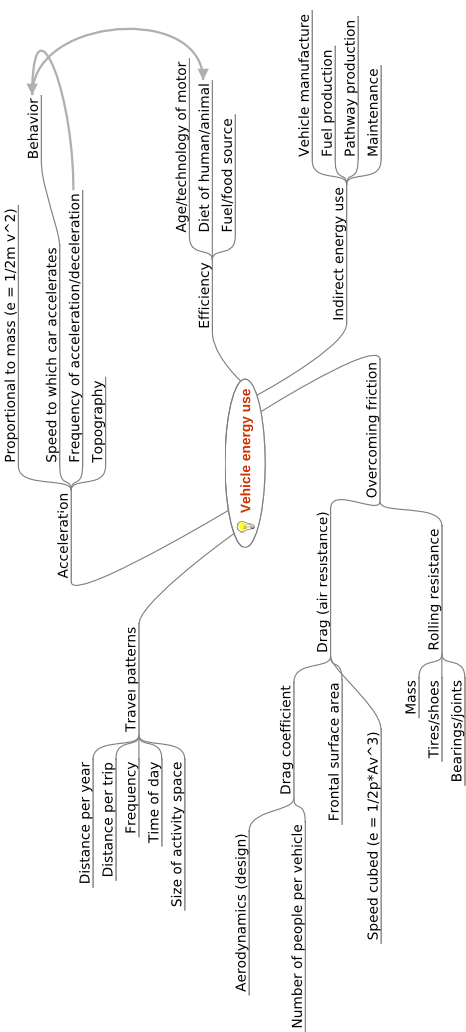
\includegraphics[width=7 cm]{schematic-energy}\end{center}
 % cc-trans.png: 1113x529 pixel, 72dpi, 39.26x18.66 cm, bb=0 0 1113 529
 \caption{Schematic diagram of the factors causing energy use in transport.}
 \label{fig:trans-schema}
\end{figure}

\subsection{System boundaries} \index{system boundaries}
As emphasised in \cref{Chapter1}, transport does not happen in isolation from
the wider world. External considerations such as friends, family and quality of
life all affect the commuter patterns people follow. The same is true of
energy use. Let us consider a car journey as an example: does one only include the
chemical energy stored in the petrol burned in the pistons? Or do we also
include the primary energy consumed in getting the fuel out of the ground and
into the petrol tank?\footnote{The extraction costs include
searching for the oil, the embedded energy in the pipelines, drilling rigs,
personnel and refinery processes. The distribution costs include diesel or
electric pumps to force the oil to flow, shipping and trucking costs and even
the embedded energy of the roads and ships needed to enable these systems to
function.}
Do we include the energy costs required to feed active travel modes? Cooking
requirements? The embodied energy in vehicles, roads, footpaths and railways?
The costs of decommissioning disused vehicles, or the net energy they save
through recycling?
The list could go on and on, to include seemingly distant energy costs such as
washing machine and shower usage, influenced by whether the transport mode is
active or passive. Taken to its extreme, it could even include knock-on impacts
through society, such as shopping patterns, holiday destinations, health and
the reshaping of social space \citep{Illich1974}.
% Could add a footnote for each!!!

What is clear from the above is that the energy costs of transport is not the
simple hard-and-fast science that it appears at the outset. It is complex. A
conceptual framework is needed to deal with this complexity and help decide
which factors to include in the analysis and which ones to leave out.
A useful analogy of this comes from economics: the price of goods can
vary depending on whether the additional costs incurred by ownership
are taken into account, let alone externalities such as pollution,
bureaucracy and disposal \citep{Perman2003}.
The costs of personal transport can be divided into variable and
fixed costs, which in turn are sub-divided (\cref{fcar-patterned}).
The precise proportion of the total cost attributable to each of these
is variable depending on the type of car and the regulatory framework
in the country in which the car is
used.\footnote{In The USA, for example,
fuel accounts for roughly one sixth of the overall lifetime cost;
in the European Union and Japan, higher taxes push this up, to over a
third \citep{Smil1993}.
}
However, because only a couple of these costs are highly
visible to consumers
(the initial price of the car and the petrol), the wider system costs are often
forgoten. The same is true of energy costs. 

\begin{figure}[h]
 \begin{center}
 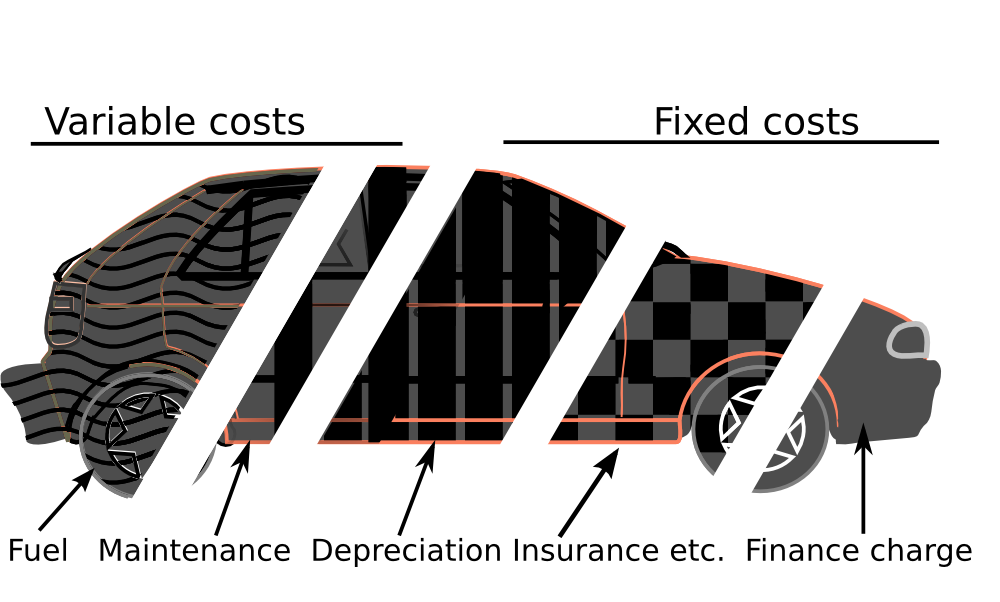
\includegraphics[width=12 cm]{car-patterned}\end{center}
 % cc-trans.png: 1113x529 pixel, 72dpi, 39.26x18.66 cm, bb=0 0 1113 529
 \caption[Relative importance of fixed and variable costs
of car ownership]{Rough approximation of relative importance of fixed and
variable costs of car ownership in the USA, based on
 \citet[p.~114]{Smil1993}. Car image from openclipart.org.}
 \label{fcar-patterned}
\end{figure}

A systematic method for analysing system level energy costs is
provided by the framework of \emph{system boundaries}
\citep{Ekvall2004-lifecycle}. 
The system boundaries determining the energy costs
of personal transport can be visualised as a set of concentric components,
whose magnitude tends to reduce, but become less certain, from the centre to
the edges \cref{f:sysbound}. The order of components in \cref{f:sysbound} has
been selected to reflect their ease of quantification and uncertainty (these
tend to increase from the inner component of direct fuel use to the outer
category of vehicle disposal). This order of energy-use components has
influenced the decision of which ones to include in the analysis: vehicle
disposal costs are small and difficult to calculate, so probably not worth
calculating. The indirect energy costs of fuel, vehicle and road production are
larger and probably easier to estimate, so more attractive for inclusion in
energy analyses of the transport. (This explains why these indirect energy
costs are quantified in \cref{ssystemlevel}, while others were not.) Still, it
is important to remember that most energy analyses of transport
systems include only the direct energy costs, so any expansion of energy cost
estimates beyond this single component should be advocated.
The direct energy cost of fuel use is always the easiest, and usually the
largest, energy use component, however. For this reason it is considered first.

\begin{figure}[h]
 \begin{center}
 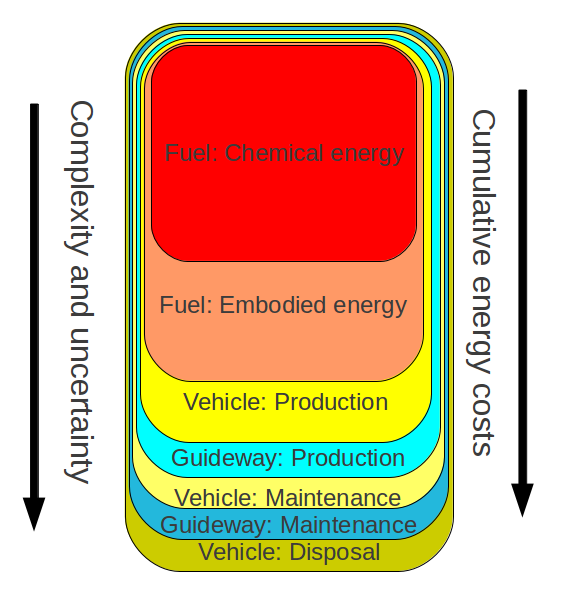
\includegraphics[width=9 cm]{sysbound}\end{center}
 % cc-trans.png: 1113x529 pixel, 72dpi, 39.26x18.66 cm, bb=0 0 1113 529
 \caption{Schematic of physical system boundaries in personal
 transport systems.}
 \label{f:sysbound}
\end{figure}

\subsection{Early quantifications of energy use in transport}
% \subsection{Fuel/food use per unit distance}
The energy costs of different travel modes have been investigated since the
advent of motorised travel, in the form of
railways.\footnote{Engineer Thomas Tredgold, for example,
went to great
lengths to calculate the efficiency of the steam engines of the day, expressing
the result not in terms of `energy' (a term which was still more commonly
used to describe individual enthusiasm and mental effort) but in terms of
coal use. His intuitive and practical unit of choice for efficiency
was lbs of coal used for a day's horse work.
% !!! convert this into mj per km??? would love to
The results of his investigations show an early interest in
efficiency and wastage:
``From the various causes of loss of effect, the quantities we have given
may be increased about 30 percent, making the coals equivalent to the
day's work of a horse 123 lbs. in the best locomotive engines likely to be
invented.

As for the engines on the Newcastle rail-roads, they at an average consume
at least twice the last quantity to do the same work''
\citep[p.~82]{tredgold1835practical}.
}
Since then there have been
a number of estimates and a great deal of speculation about which forms of
travel are most efficient. However, there still remains little hard data
about real-world performance of different modes.

The first comprehensive study into the energy impacts of personal travel
that could be found was \citet{Fels1975}. This detailed paper built on earlier
work that investigated the energy costs of automobile manufacture
\citep{Fels1973}. The study was pioneering
in its inclusion of a wide range of indirect energy costs, and in the 1975
paper, these were calculated for the main US modes of transport. \Cref{t:fels}
shows the results. This has been used (although not as much as one may have
expected, given the importance of transport) as an input in subsequent
studies (e.g.~\citealp{Fels-referal-1985}). Although seriously outdated by
now, this research provide a benchmark against which more recent estimates
and methods can be compared.

% \begin{table}[h]
% \centerline{}
% \caption{The direct and indirect energy costs of personal travel
% \citep{Fels1975}.}
% \begin{tabular}{p{2.1cm}rrrrrrrrl}
% \toprule
%  Mode $\Rightarrow$ & \multicolumn{1}{c}{Car} & \multicolumn{1}{l}{} &
% \multicolumn{1}{l}{} & \multicolumn{1}{l}{} & \multicolumn{1}{c}{Taxi} &
% \multicolumn{1}{l}{} & \multicolumn{1}{l}{} &
% \multicolumn{1}{l}{} & \\
% Contribution (kWh/m) $\Downarrow$ & \multicolumn{1}{l}{Big} &
% \multicolumn{1}{l}{Small} & \multicolumn{1}{l}{City bus} &
% \multicolumn{1}{l}{Rail} & \multicolumn{1}{l}{Petrol} &
% \multicolumn{1}{l}{Diesel}& \multicolumn{1}{l}{Moto.} & \multicolumn{1}{l}{Bike}
% & Walk \\
% \midrule
% Operation  & 3.19 & 1.63 & 9.57 & 16.7 & 5.23 & 2.71 & 0.6 & 0.042 &
% \multicolumn{1}{r}{0.063} \\
% \midrule
% Vehicle manufacture & 0.39 & 0.21 & 0.3 & 0.4 & 0.54 & 0.82 & 0.05 & 0.042 &  \\
% Guideway manufacture & 0.03 & 0.03 & 0.09 & 0.7 & 0.05 & 0.05 & 0.03 & 0.014 &
% \\
% \midrule
% Total per vehicle mile & 3.61 & 1.87 & 9.96 & 17.8 & 5.82 & 3.58 & 0.68 & 0.098
% & \multicolumn{1}{r}{0.063} \\
% \bottomrule
% \end{tabular}
% \label{t:fels}
% \end{table}

\begin{table}[h]
\centerline{}
\caption[The direct and indirect energy costs of personal travel
\citep{Fels1975}]{The direct and indirect energy costs of personal travel
\citep{Fels1975}. (Original values  converted into SI units
(1 $kWh/mile$ = 2.237 $MJ/km$).}
\begin{tabular}{p{2.1cm}rrrrrrrrl}
\toprule
 Mode $\Rightarrow$ & \multicolumn{1}{c}{Car} & \multicolumn{1}{l}{} &
\multicolumn{1}{l}{} & \multicolumn{1}{l}{} & \multicolumn{1}{c}{Taxi} &
\multicolumn{1}{l}{} & \multicolumn{1}{l}{} &
\multicolumn{1}{l}{} & \\
Contribution ($MJ/km$) $\Downarrow$ & \multicolumn{1}{l}{Big} &
\multicolumn{1}{l}{Small} & \multicolumn{1}{l}{City bus} &
\multicolumn{1}{l}{Rail} & \multicolumn{1}{l}{Petrol} &
\multicolumn{1}{l}{Diesel}& \multicolumn{1}{l}{Moto.} & \multicolumn{1}{l}{Bike}
& Walk \\
\midrule
Operation  & 7.14 & 3.65 & 21.41 & 37.36 & 11.70 & 6.06 & 1.34 & 0.09 & \multicolumn{1}{r}{0.14} \\
Vehicle manufacture & 0.87 & 0.47 & 0.67 & 0.89 & 1.21 & 1.83 & 0.11 & 0.09 & - \\
Guideway manufacture & 0.07 & 0.07 & 0.20 & 1.57 & 0.11 & 0.11 & 0.07 & 0.03 & - \\
Total per vehicle mile & 18.06 & 9.36 & 49.84 & 89.07 & 29.12 & 17.91 & 3.40 & 0.49 & \multicolumn{1}{r}{0.32} \\
\bottomrule
\end{tabular}
\label{t:fels}
\end{table}

The main problem with Fels' estimates is that they do not match the current
transport system in either space of time. Manufacturing techniques have
advanced drastically in the intervening 40 years and it is clear that the UK
fleet and roads are different from those of the USA, where things are larger.
Therefore the numbers presented in \citet{Fels1975} are
used only for comparison with more recent energy use data.

\section{Direct energy use: published estimates} \label{sdirecte}
\index{energy use!direct}
Official UK data on the energy costs of transport were not easy to find.
Because of this issue, the initial approach was to search for published
estimates of energy costs of each mode, one by one. This resulted in a
`patchwork' of results, with a different source for each mode (\cref{tmodes}).
There are numerous inconsistencies of date, place and method of data collection
in this dataset, but it was the best that could be found throughout the
majority of the thesis. The planned approach to this data quality issue was to
follow \citet{Lovelace2011-assessing} and accept the uncertainty of the estimates and
take them into account using sensitivity analysis. %!!! DB says incorporate into PhD!

\begin{table}[t]
\caption{Direct energy use of selected modes}\centering{
\begin{tabular}{lr}

Mode & Ef (MJ/vkm)\\ \hline

Bicycle & 0.093$^a$  \\
Bus & 7.34$^b$  \\
Car & 2.98$^c$  \\
Metro & -- $^d$  \\
Motorbike & 1.87$^e$ \\
Train & 63.4$^b$ \\
Walking & 0.13$^a$ \\

\end{tabular}}
\label{tmodes}
\begin{footnotesize}

\vspace{1cm}
 a: \citep{Coley2002}, b: \citep{Hansard2005}, c:
\citep{MacKay2009}, d: \citep{DfT2011-commuting}, d:
\citep{LondonUnderground2007}, e: \citep{ORNL2011}
\end{footnotesize} %!!! Make this more diferent from table:modes!!!
\end{table}


In early 2013 a better data source was discovered
\citep{Defra2011}.\footnote{Thanks to Alex Singleton, who mentioned the dataset
during a talk on the CO$_2$ emissions from the school commute at the `GISRUK2013'
conference. This dataset was also used by \citet{smith2011polycentricity},
to calculate the CO$_2$ emissions from travel to work at the geographical
level of administrative wards.
}
Although the Defra dataset is primarily concerned with greenhouse gas
emissions with the aim of complying with the 2008 Climate Change Act,
CO$_2$ and energy use are two sides of the same coin. In fact,
emissions factors of different fuels per unit energy are contained within the
same report. This allows
for direct conversion into energy costs, without needing to pass
through the usual intermediary stage of volume, when the type of fuel is known.
The emissions allocated
to each major mode of motorised transport (excluding cars)
and some sub-divisions are presented in \cref{tghgfactors}.
This dataset is extremely useful, as it already takes into account
variations in occupancy and vehicle specification, allowing average numbers to be used.
Also, geographic variation
is accounted for to a limited extent through the distinction between sub-modes
(i.e.~light rail/tram vs Underground, local bus vs London bus and regular taxi
vs black cab, the latter of which dominate in London).

\begin{table}[htbp]
\caption[Direct greenhouse gas emissions by mode]{Direct greenhouse gas
emissions associated with different forms of
personal transport \citep{Defra2011}.}
\begin{tabular}{llrrrr}
\toprule
\multicolumn{1}{c}{Mode $\Downarrow$} & \multicolumn{1}{c}{\textbf{kg~CO$_2$
eq./pkm $\Rightarrow$}} & \multicolumn{1}{c}{\textbf{CO$_2$}} &
\multicolumn{1}{c}{\textbf{CH4}} & \multicolumn{1}{c}{\textbf{N2O}} &
\multicolumn{1}{c}{\textbf{Total}} \\
\midrule
Taxi & Regular Taxi  & 0.14626 & 0.00004 & 0.00126 & 0.14756 \\
 & Black cab & 0.15587 & 0.00003 & 0.00118 & 0.15709 \\
Bus & Local bus  & 0.12269 & 0.00013 & 0.00098 & 0.12380 \\
 & London bus & 0.08201 & 0.00007 & 0.00055 & 0.08263 \\
 & \textbf{Av. local bus} & \textbf{0.11097} & \textbf{0.00012} &
\textbf{0.00086} & \textbf{0.11195} \\
 & Coach & 0.02810 & 0.00007 & 0.00057 & 0.02874 \\
Rail & National rail & 0.05501 & 0.00005 & 0.00312 & 0.05818 \\
 & International rail  & 0.01502 & 0.00001 & 0.00009 & 0.01512 \\
 & Light rail/tram & 0.06709 & 0.00003 & 0.00041 & 0.06753 \\
 & Underground & 0.07142 & 0.00004 & 0.00044 & 0.07190 \\
Ferry & Foot passengers & 0.01912 & 0.00001 & 0.00015 & 0.01928 \\
 & Car passengers & 0.13216 & 0.00004 & 0.00101 & 0.13321 \\
 & \textbf{Average} & \textbf{0.11516} & \textbf{0.00004} & \textbf{0.00088} &
\textbf{0.11608} \\
 \bottomrule
\end{tabular}
\label{tghgfactors}
\end{table}

Further breakdowns of this data (by car model, bus region and
occupancy level of trains, for example) are contained within 
this report.\footnote{Notable
examples of the level of breakdown include the type of train: national rail,
international rail (Eurostar), light rail and tram and London Underground
are each included. Converting CO$_2$ emissions into energy use in the
electrified cases rely on best estimates of the carbon intensity of grid
electricity.
}

In terms of car energy use,
energy costs can be broken down to the level of
emission tax band, from A (``mini'') to I (``MPV'') for diesel and petrol
cars and if the fuel type of the car is unknown. Emission factors
convertible into energy are also provided for cars with the following
alternative fuel types: hybrid, LPG (Liquified Petroleum Gas)
and CNG (Compressed Natural Gas). (Interestingly, no emissions estimates
are provided for battery-electric vehicles (BEVs) or electric
bicycles, which are both growing in market share and have been touted for
their energy performance.) \index{bicycle!electric}

The most important categorisation of cars from the perspective of the Understanding
Society dataset (USd), the primary source of individual level microdata in this project,
is into small, medium and large cars. These categories are used
to classify vehicles at the household level (variable ensize1 in the USd).
The three bands are deemed to be a suitable level of simplification to model and improve
understanding of energy use in transport, and can account for variations
in the vehicle fleet in different areas. No fuel type is specified in
the USd, so the average energy use ($Ef$) of each engine band was calculated.
The following equation was used:
\begin{equation}
\overline{Ef} (MJ/vkm) = \displaystyle{\sum_{ft}}
P_{ft} \times
\frac{kg~CO_{2}}{vkm}_{ft} \times \frac{MJ}{kg~CO_2}_{ft}
\label{eqmjco2}
\end{equation}
where $ft$ represents fuel type (in this case only petrol or diesel, although
more fuel types could be included as their market share increases), $P$ is the
market share of the fuel type, and $\frac{kg~CO_{2}}{vkm}_{ft}$ and $\frac{MJ}{kg~CO_2}_{ft}$
represent the known emissions per kilometre and energy release per kg~CO$_2$ released
of the particular fuel type in question,
respectively.\footnote{The
first two arguments of this equation are displayed
in \cref{tdefracar}. The CO$_2$ emissions resulting per unit of energy use
are provided by \citep[Table 1c]{Defra2011} as 0.23963 and 0.24989
kg~CO$_2$ / kWh for petrol and diesel respectively. To convert this into
MJ per kg~CO$_2$ emitted, the final argument of \cref{eqmjco2}, take the inverse
and multiply by 3.6 (the number of MJ in one kWh): 15.0 and 14.4 MJ/kg~CO$_2$
for petrol and diesel respectively. Values for ``100\% mineral petrol''
and ``100\% mineral diesel''
were used rather than biofuel blends as the undiluted product still dominates
the market and is less susceptible to variability over time.
}
The closeness of the average energy costs of driving reported by \citet{MacKay2009}
(presented in \cref{tmodes}) and our own estimates calculated through \cref{eqmjco2}
and presented in \cref{tdefracar} (2.98 and 3.02 MJ respectively) provide confidence
in the suitability of our method.
 

\begin{table}[htbp]
\caption[Conversion table from emissions to energy use by size of car]
{Conversion table from emissions (kg CO$_2$/km,
presented in the first three columns of data) to energy use by size of car,
based on \cref{eqmjco2}.
Emissions data and conversion tables from \citet{Defra2011}.}
\begin{center}
\begin{tabular}{llrrrrr}
\toprule
\multicolumn{ 2}{l}{Engine size $\Downarrow$ Fuel $\Rightarrow$} & \multicolumn{1}{l}{Petrol} & \multicolumn{1}{l}{Diesel} & \multicolumn{1}{l}{Unknown} & \multicolumn{1}{l}{$P_{Petrol}$} & \multicolumn{1}{l}{Energy use} \\
Units $\Rightarrow$  & &\multicolumn{3}{c}{Emissions (${kg ~CO_{2}}/{vkm}_{}$)} & (\%) & ($MJ/vkm$) \\
\midrule
\multicolumn{ 2}{l}{Small ($<=$ 1.4 l)} & 0.170 & 0.143 & 0.166 & 83.3 & 2.47 \\
\multicolumn{ 2}{l}{Medium (1.41 to 2.0 l)} & 0.211 & 0.179 & 0.200 & 65.9 & 2.97 \\
\multicolumn{ 2}{l}{Large ($>$ 2.0 l)} & 0.298 & 0.242 & 0.268 & 46.8 & 3.95 \\
\multicolumn{ 2}{l}{Weighted average} & 0.208 & 0.192 & 0.203 & 72.7 & 3.02 \\
\bottomrule
\end{tabular}\end{center}
\label{tdefracar}
\end{table}

Because larger cars are more likely to have diesel engines, it is not adequate
to assume that the petrol/diesel split (which is roughly 3:1)
remains constant over all car classes. \citet{Defra2011} do not state
explicitly what proportion of cars are diesel in each category, so this
information was calculated using the following re-arrangement:
\begin{equation}
 \overline{Ef} = P_{ft1} \times E_{ft1} + P_{ft2} \times E_{ft2}
\end{equation}
\begin{equation}
  P_{ft1} = \frac{\overline{E} - E_{ft2}}{E_{ft1} - E_{ft2}}
\end{equation}
where $E$ are the emissions per unit distance and $P$ is the proportion of cars
in each fuel type ($ft$). The results, also shown in \cref{tdefracar}, show that
it is dangerous to assume that the 3:1 petrol:diesel split remains constant over
all car classes and in all areas.

The methodology to convert the CO$_2$ costs presented \cref{tghgfactors} for
buses, trains, trams and taxis is simpler
than that used for cars because there are fewer sub-divisions within the other
modes of transport.
Also, a single fuel type can be assumed in most cases.\footnote{The
dataset is less useful for trains because the emissions of trains combine
both electric and diesel power sources. A separate government document
states that ``CO$_2$
emissions from diesel trains make up almost 90\% of rail GHG emissions''
\citep[p.~13]{DfT2011-train90}. Electric trains have only marginally
lower emissions --- between 20 and 35 percent \citep{Hickman2012-trains} ---
and some trains still rely on coal and gas oil (pushing emissions in
the opposite direction) \citep{DfT2011-train90}. These facts suggest that
assuming all national trains are powered by diesel would provide a reasonable estimate
of the overall average energy costs.
The energy costs of international rail is a different matter not tackled here
as few people commute internationally by train.
}
A major difference between the energy cost estimates for cars and other
modes is occupancy: the figures presented in \cref{tdefracar} apply per vehicle
whereas those calculated for other forms of transport apply per person.
This is a major advantage of using the Defra data rather than the variety of
sources referenced in \cref{tmodes}: occupancy has already been carefully
factored in based on UK conditions by Defra, reducing the need to identify
occupancy figures at the national level and then decide which are the most
reliable.\footnote{Clearly
occupancy also varies from region to region and depending on the
time of travel. For the purposes of modelling energy use, however,
a single national number is a good place to start.
}

\begin{table}[htbp]
\caption[Emissions data and calculated energy use of motorised
modes]{Conversion of CO$_2$ emissions data to energy use for motorised
modes of transport. Data from \citep{Defra2011}}
\begin{center}
\begin{tabular}{lrlp{1.8cm}p{1.8cm}p{1.8cm}}
\toprule
Mode & Emissions & Fuel type & Carbon content & Energy content & Energy use \\
Units $\Rightarrow$ & $\frac{kg CO_2}{pkm}$ & - & $\frac{kg CO_2}{kWh}$ &$\frac{MJ}{kg CO_2}$ &
$\frac{MJ}{pkm}$ \\
\midrule
Bus (local) & 0.14754 & Diesel & 0.25 & 14.41 & 2.13 \\
Coach	& 0.03000 & Diesel &	0.25	& 14.41 &	0.43\\
Motorbike & 0.11606 & Petrol & 0.24 & 15.02 & 1.74 \\
Taxi & 0.21040 & Diesel & 0.25 & 14.41 & 3.03 \\
Train  & 0.05340 & Diesel & 0.25 & 14.41 & 0.77 \\
Tram & 0.07101 & Electricity  & 0.45 & 8.08 & 0.57 \\
\bottomrule
\end{tabular}\end{center}
\label{tdefra2}
\end{table}

With estimates of the energy costs of different modes, the next stage is to
calculate the energy costs per trip. The average
direct energy used per trip ($ETf$) is a simple function of the fuel
energy use of the mode in question multiplied by the distance:
\begin{equation}
 ETf(i,j) = 2 dR(i,j) \times Ef
\label{eq:et}
\end{equation}
where $Ef$ is the fuel energy used per kilometre by mode and $dR(i,j)$ is
the route distance between points i and j. The value is multiplied by two
because trips to work are two way. \Cref{Chapter6} %!!! yes
describes how this equation can be used as the basis for estimating total
energy costs over the course of the year. The next stage, however, is to
look into the indirect energy costs of personal travel.

\section{Calculating system level energy use} \label{ssystemlevel}
As described in \cref{sfundamentals}, transport consumes energy through a
wide range of pathways, only the most obvious of which ---
energy directly consumed in vehicle engines for propulsion --- is covered by official
statistics\footnote{Even
in terms of direct energy use of transport the governments statistics are limited.
As described in the previous section, geographical breakdowns do not extend
below the coarse Local Authority level, or to non-road modes. There is no
initiative to report energy or emissions by reason for trip, making it hard
for transport planners and other decision makers to know where to focus
mitigation strategies. Also, energy use is not reported directly but as emissions.
This means that
researchers interested in energy must convert
emissions factors into energy use, as was done in the previous section.
}
and the majority of energy-transport
research (e.g.~\citealp{schipper1992energy, Wohlgemuth1998, Hickman1999, Brand2013}).
The discussion presented in \cref{sfundamentals} makes it clear that not all
indirect energy impacts can be realistically quantified. Therefore only a subset of
the indirect energy costs of commuting is included in this section. The three most
important and easily quantified costs are:
\begin{itemize}
 \item the energy costs of fuel and food production ($Efp$)
 \item the energy costs of vehicle manufacture ($Ev$)
 \item the energy costs of guideway manufacture (e.g.~roads and railways) ($Eg$)
\end{itemize} 

For the purposes of simplicity, it can be assumed that the system level energy
costs equal the sum of these indirect energy costs and direct energy costs:
\begin{equation}
 Esys = Ef + Efp + Ev + Eg
 \label{eqesys}
\end{equation}
This formula requires that all arguments are provided in the same units.
The direct energy costs of personal transport are calculated above in SI
units of megajoules per passenger kilometre (MJ/pkm). Yet the energy costs of
producing a car or building a road is generally reported as a single energy
expenditure (e.g.~$\sim$300 GJ per car) and not per unit distance.
The first paper that formalised this problem in the context of system level
energy costs of transport was by \citet{Fels1975}, so the calculation of
energy costs in this thesis is strongly influenced by this paper.
Formally, the total (system level) energy use for each trip ($Esys$) can be
defined, for each mode ($m$), as follows \citet{Fels1975}:
\begin{equation}
Esys_m =  Ef_m +  \frac{EMv_m}{Lv_m} + \frac{EMg_m}{Lg_m}
\label{eq:esys}
\end{equation}
where $EMv$ and $EMg$ are the `one-off' embodied energy costs of
vehicles and guideways and
$Lv_m$ and $Lg_m$ are their lifespans,
measured in kilometres and vehicle-passes (the number of passing vehicles a road
can take before it needs to be replaced), respectively.
It should be instantly clearly that \cref{eqesys} is a simpler and
more generalised version
of \cref{eq:esys}, and indeed it is derived from Fels' work, where
\begin{equation}
 Ev = \frac{EMv}{LV} \hspace{3cm} and  \hspace{3cm} Eg =
\frac{Emg}{Lg}.
\end{equation}
\citet{Fels1975} did not include the energy costs of fuel production, despite
the size of this component.

The above equations can be used to calculate
system level energy costs for single trips to work and back ($ETsys$):
because $Esys$ is provided in the same units as $Ef$, one simply replaces the
latter with the former in \cref{eq:et}. %!!! DB:reword
However, the calculation of
system level energy costs is rarely undertaken, and merits further comment
before
discussing the data that enable system level energy costs to be estimated. 

Fels' framework for calculating system level energy costs has been available
to researchers for almost 40 years. Despite this, most researchers
continue to use only direct energy
costs in their analysis (notable exceptions include
\citealp{Treloar2004, Lenzen1999, MacKay2009, Lovelace2011-assessing}). %!!! again...
This reluctance to engage with system level energy
costs can be attributed to a variety of factors, the most important
of which are probably the invisibility of indirect energy costs,
the tendency to favour simple, easy energy calculations and uncertainty.
Uncertainty is the most critical of these: it is fine to have formulae
that \emph{can} work out
system level energy costs, but this is only useful if the input data is
sufficiently reliable. The bulk of this section is therefore dedicated
to describing the evidence that is available on indirect energy costs of food
and fuel production, vehicle manufacture and the infrastructure these
vehicles rely upon. It is acknowledged that this adds complexity to the energy
analysis, but the complexity can be justified: indirect
energy costs of vehicle production and road construction can have a large
impact on total energy use calculations
\citep{Lovelace2011-assessing, Lenzen1999, Wee2000}, with associated impacts
for climate change and energy security. The ultimate aim is to provide
estimates of indirect energy costs per passenger kilometre (pkm) of
different modes. These estimates serve as inputs into energy use
calculations based on distance and mode, allowing the user to choose whether
to focus attention on direct or indirect energy use (\cref{screengrab-final-e}).
The results of these equations are given after evidence on
the magnitude of indirect energy costs has been presented, in \cref{tfinale}.

\begin{figure}[t]
 \begin{center}
 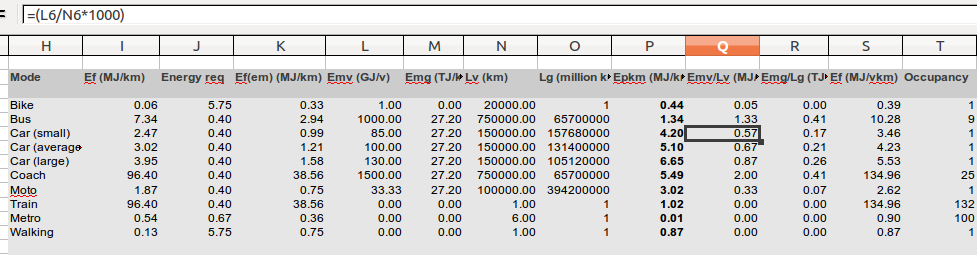
\includegraphics[width=14 cm]{screengrab-final-e}
\end{center}
 % cc-trans.png: 1113x529 pixel, 72dpi, 39.26x18.66 cm, bb=0 0 1113 529
 \caption{Screen shot of the spreadsheet used to calculate system level energy
 costs.}
 \label{screengrab-final-e}
\end{figure}

% Note that the above equations measure energy use per vehicle trip, yet
% commuting is measured as person trips.\footnote{
% This is a subtle difference because, in many cases, $Etv$ and $Et$ are the same
% thing (i.e. the vehicle has one occupant). However, it is important to
% distinguish the two because average occupancy is greater than 1 in cars due to
% trip sharing, and much greater than one in public transport.}
% The energy costs per vehicle trip ($Etv$) are converted into estimates per
% passenger trip ($Et$) by dividing by the occupancy rate (p). Average values of
% the the variables presented in \cref{eq:et} and occupancy ($Oc$) are
% presented in Table \cref{table:modes}:
% The above formulae allow
% meaning to be extracted from otherwise incommensurable energy values by making
% sense of, adding context to and converting into a single (per unit distance)
% comparable unit the various indirect energy cost estimates presented below.

\subsection{The embedded energy of fuel} \index{energy use!fuel production}
\label{sfuelem}
In the context of multi-mode transport energy costs, `fuel' here refers not
only to petrol and diesel, but to electricity and food as well. It is all too easy
to assume that vehicles only use the energy released by the degradation of
these low-entropy resources. However, each of these fuel sources require very
large energy inputs before they are available at the point of use.

\subsubsection{Liquid fuels} \index{fuel}
Liquid fuels, which dominate transport energy costs, consume a huge amount of
energy even before they are burned in the oxygen-rich atmosphere. In fact,
``the oil and gas industry is traditionally the most energy-using industry'',
at least in the USA \citep{Guilford2011}. Most of these
inputs are hidden from public view: consumers only interact with the end
product and even then it is kept out of sight by petrol pumps and hidden fuel
tanks. Energy is used during every stage however: in prospecting, drilling,
pumping, refining, transport and, increasingly, enhanced oil recovery (EOR),
horizontal drilling and bitumen processing techniques. In layman's terms,
previous estimates include ``only the energy in the
petrol, not the energy used at the oil refinery that makes the petrol, nor the
energy used in trundling the oil and petrol from A to B''
\citep[p.~104]{MacKay2009}. The transformation of
crude oil from a far-flung deposit of variable quality into a finished product
is difficult to follow. Its energy costs are therefore variable over time and
space \citep{Cleveland2005}; the same would apply to food or any other `fuel',
all of which require energy to produce. The aim in this section, therefore, is
to find best estimates of energy costs, rather than exact answers. The
few studies that are dedicated to these costs tend to use round numbers and
avoid error bars, emphasising that the level of uncertainty in their estimates
is unknown.
% Image of oil industry system

Estimates of the energy costs of producing liquid fuels products have been
undertaken by a number of researchers. \citet{Cleveland2005} aimed \index{EROEI}
at estimating the energy return on energy investment (EROEI) of American crude
oil production over time, based on data from the Census of Mineral Industries.
This is an unusually detailed dataset, which ``reports the quantities of fuel
and electricity used in the petroleum sector at 5 year intervals from 1954 to
1997'' \citep[p.~777]{Cleveland2005}. The findings show that oil is
energy intensive to produce and that these costs have increased
over time, rising from 1/20$^{th}$ to 1/11$^{th}$ (EROEI values of 20:1 and 11:1) of
the overall quality-adjusted energy content of crude oil between the 1970s and
1990s. Building on this study, \citet{Guilford2011} employed new datasets and
methods to update the EROEI estimates into the 21$^{st}$ century. They also found
long-term increases in oil production energy costs, reaching 1/10$^{th}$ of the
energy content of the crude oil by 2007.
Such detailed datasets of oil industry energy use are not available for the UK,
let alone worldwide, so the study should be used as guidance only. There has,
however, been one preliminary study of the energy costs of global oil
production, which broadly supported Cleveland's findings. In it, the
EROEI of crude oil production was found to have dropped from
26:1 in 1992 to 18:1 in 2006: clear evidence of increasing indirect energy
costs \citep{Gagnon2009}.

It is important to
remember that the aforementioned EROEI studies focussed only the energy costs
of crude oil production: refining, distribution and
other costs are omitted, so the `well-to-wheel' costs would be substantially
higher. This problem is tackled in the life cycle analysis (LCA) literature
for biofuels (e.g.~\citealp{cherubini2009energy}), but no study dedicated to the
EROEI (or simply EROI as it is sometimes called) could be found
for the main transport fuels, petrol and diesel. Yet it would make little sense
to use values for crude oil production at the well head when in fact cars use
much lighter products at the petrol pump. The latter require far more complex
and energy intensive processes than pumping the oil alone. More research is
needed into the energy costs of liquid fuel production overall. However, this
is not the place to conduct such an overdue energy analysis. Instead, 
`best' (most reliable and broadly accepted in the
academic community) estimates from the literature must be relied upon.
This seems to be the approach taken by Professor David
MacKay also, who uses an EROEI value of 2.5 for
transport fuels taken from a previous study. He provides the following
justification: ``It’s been estimated
that making each unit of petrol requires an input of 1.4 units of oil and
other primary fuels (Treloar et al., 2004)''
\citep[p.~30]{MacKay2009}.\footnote{This
estimate
is in fact based on an earlier study: ``a primary energy factor
of 1.4 was assumed for all liquid fuels, as it takes 1.4 GJ of oil
and other primary fuels to make 1 GJ of petrol \citep{Treloar1997}''
\citep[p.~46]{Treloar2004}. The 1997 article (which is highly cited)
could not be accessed, however, so the opinion of David MacKay that this
estimate is reliable was deferred to in this case. The search for this number
reveals a wider question: how can such an important number be so little
researched and so hard to find?
}
This estimate is neither up-to-date nor based on UK data. However, in the
absence of comprehensive \emph{well-to-wheel} energy analyses for diesel and
petrol production, it appears to be the best source available, implying that
$Efp$ = $Ef \times 0.4$ for modes that burn petrol and diesel. More up-to-date
estimates should be included as soon as they emerge.

\subsubsection{Food} \index{food} \index{bicycle}
Bicycles and walking are sometimes portrayed as `zero emission' travel options.
This statement is clearly misleading, on several levels. Bicycle and shoe
manufacture (unless second-hand bicycles or shoes are used) take energy,
even though the implied emissions would be a tiny fraction of that emitted
from the energy costs of manufacturing a car.
In terms of direct emissions, the phrase appears, at face value, to be correct:
no pollution can be seen emanating from an accelerating bicycle, and the human
power source can be assumed to require food and drink inputs regardless of his
or her activity levels \citep{Brand2006}.
The possibility of limited correlation between food consumption and physical
activity is further supported by evidence of a worldwide `obesity epidemic'
\citep{caballero2007global}, which
implies an excessive consumption of food, and therefore energy,
amongst some of the least active members of society \citep{Michaelowa2008}.

On the other hand, it has been observed that exercise tends to increase food
consumption, although not in a linear or entirely predictable way \citep{Melzer2005}.
Given these uncertainties and caveats, past literature is relied upon.
\citet{Lovelace2011-assessing} assumed a linear %!!! include?
relationship between cycling and food energy use for the purpose of simplicity,
and this approach is continued here.
This assumption is based on the best evidence that could be found on the
subject of energy use correlates of walking and cycling,
from a widely cited paper published in \emph{Energy Policy}
\citep{Coley2002}. (The place of publication
is relevant in this case, because most literature related to energy intake and
physical activity is published in health journals, so is not directly
applicable to energy analysis.)
\citet{Coley2002} analysed this issue in detail, and concluded that it
is a mistake not to provide emission factors for walking and cycling in the
same way that they are included for motorised forms. The work estimated the
average energy intake for different activities, with the aim of providing
recommendations to overcome this shortfall.
The chemical and embodied energy of additional food used by
cyclists was calculated be 94\,kJ/km and 539\,kJ/km respectively,
assuming a fixed embodied:chemical energy ratio of 5.75.
For walking, the estimated energy costs are approximately 50\% greater:
129 and 740 kj/km respectively.
It is assumed that the change in food demand from driving is negligible.%
%%
\footnote{One
could argue that driving increases one's marginal food intake in
a similar way, but it seems that driving requires no more energy than average,
everyday activities such as housework and shopping, based on an inventory of
activity types and metabolic rate \citep{Ainsworth2000}. In fact the relative
metabolic rate of ``driving at work'' (MET = 1.5) is lower than that of many
other common activities such as ``childcare'' (MET = 2.5 - 3) and ``putting
away groceries'' (MET = 2.5) \citep{Ainsworth2003}.
}
%%\footnote{One could question the assumption that this ratio is the same for cyclists and car drivers, although quantifying such differences is currently not an option as the links between consumptive and `environmental' behaviours are far from understood \citep{Gatersleben2010}.}

These values are far from the final word on the matter, as the study failed
to account for differences in diet and food behaviours.
Cyclists, for example could be assumed
to have a more environmentally aware diet as many identify with an environmentalist
identity \citep{Gatersleben2007}. Amplifying this effect could be the issue of
food wastage: from an environmental perspective it is not the food eaten
that causes indirect energy use and emissions, but the act of purchasing the
product that drives demand. It is, of course, impossible to estimate how much more
(or less) food walkers and cyclists waste compared with those who travel by other
modes.\footnote{Data
from the Living Costs and Food Survey (LCFS) could potentially be used to
analyse the varying food buying habits of cyclists compared with non-cyclists
as it contains questions on cycling.
}
The system boundary surrounding the energy costs of food consumption could
expand even further, to include the transportation energy costs of buying the
food, which have been found to be of critical importance \citep{Coley2009}.
Again, however, this
knock-on impact is very hard to estimate and is therefore excluded from the analysis.
This explains why Coley's estimates are used here: as with the EROEI question of
liquid fuel production, the best estimate from the literature is used.
Taking Coley's (2002) values, $Efm$ for food can be assumed to be 5.75 $\times$
$Ef$ 0.74 and 5.4 MJ/pkm for walking and cycling respectively. 

\subsubsection{Electricity} \index{electricity}
The final energy source used for transportation is electricity. Currently the
share of passenger kilometres powered by the national grid is low in the UK,
amounting to just over 1\% of the total (\citealp[p.~104, table
18.3]{MacKay2009}, \cref{fdirecten}).

\begin{figure}[t]
 \begin{center}
 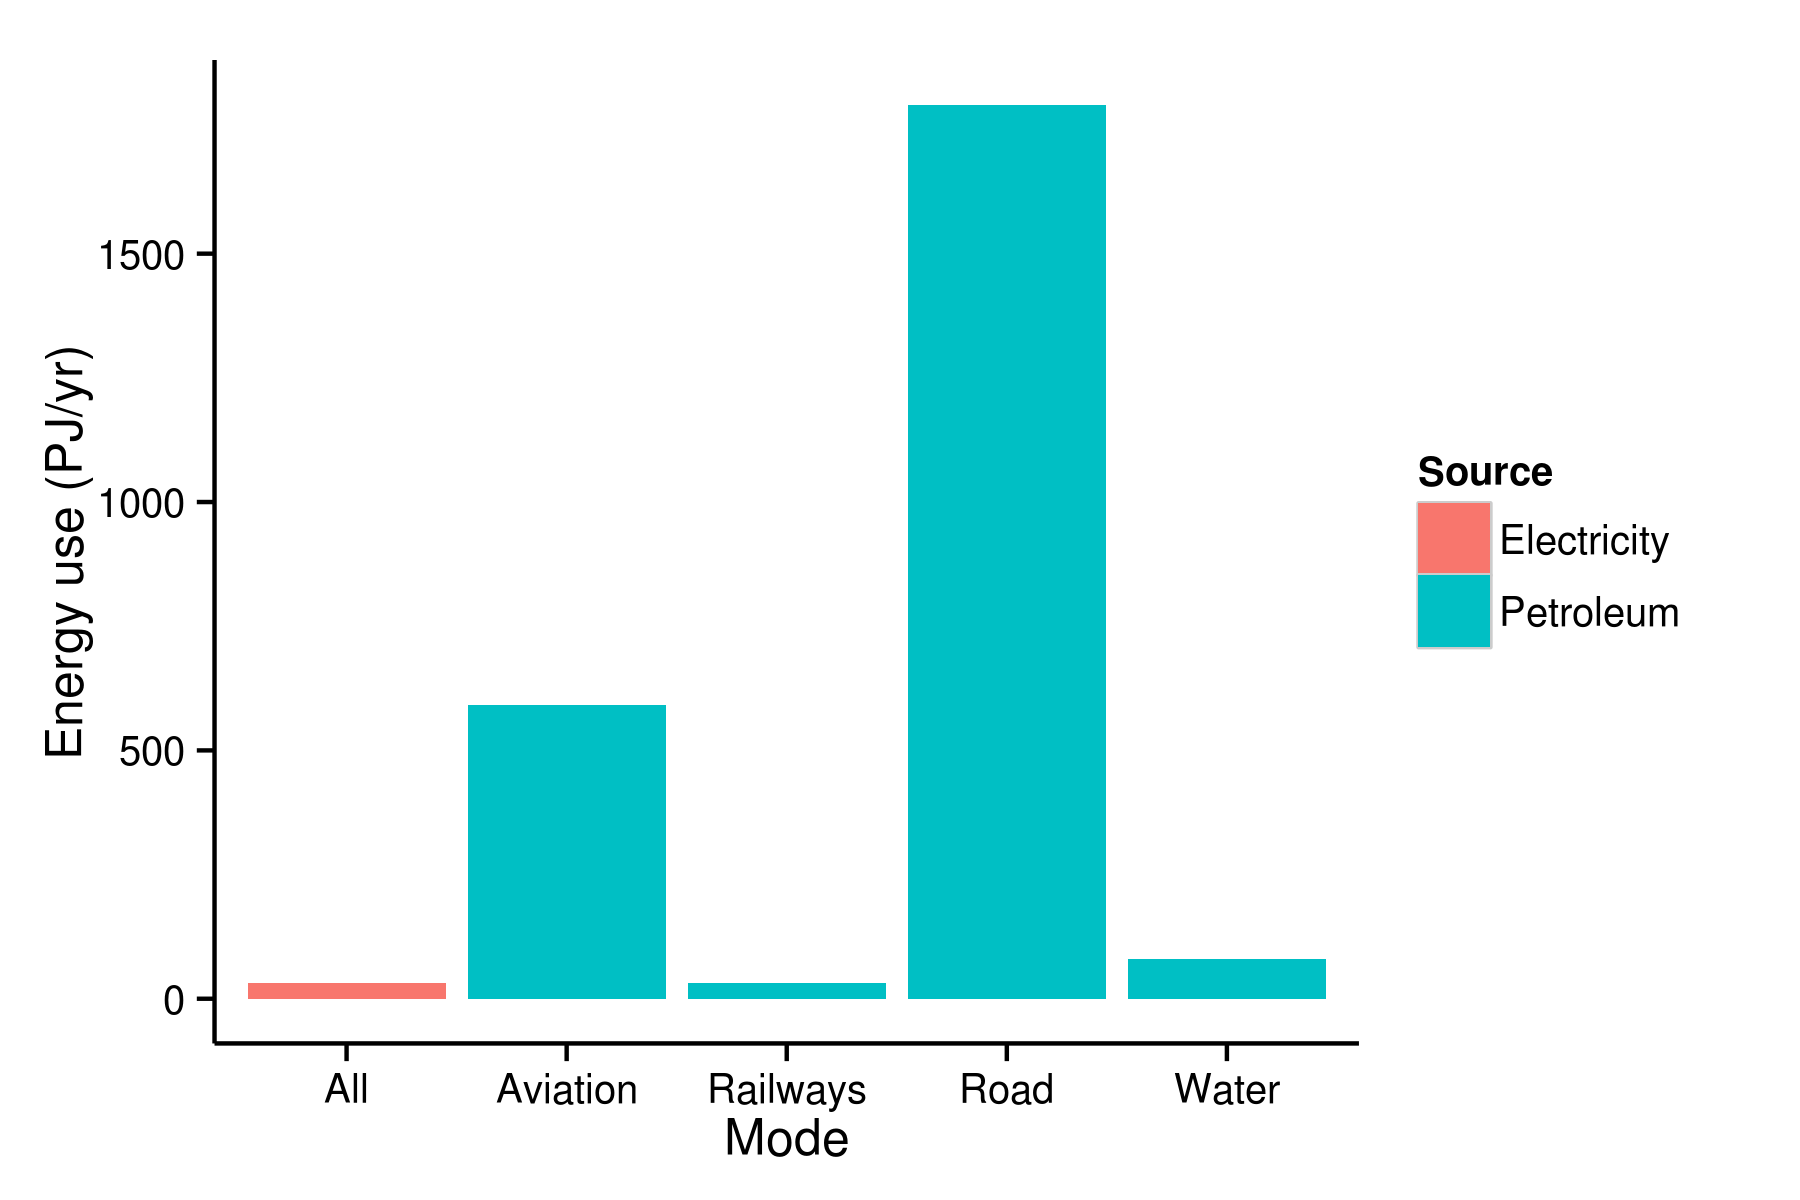
\includegraphics[width=12 cm]{direct-en}
\end{center}
 % cc-trans.png: 1113x529 pixel, 72dpi, 39.26x18.66 cm, bb=0 0 1113 529
 \caption[UK transport energy consumption by mode and energy source]{UK transport energy consumption by mode and primary energy source in
2006 \citep[p.~104]{MacKay2009}.}
 \label{fdirecten}
\end{figure}

Currently, electricity use for personal travel is limited to electric
rail and a few hundred electric cars (unless telecommuting is counted as
personal travel, which it is not in this thesis),
% \footnote{} % !!! How many?
although the proportion is forecast to grow into the future \citep{Skea2010}.
Even ignoring the future energy use of electric cars, the indirect energy costs
of electricity production must be estimated if \index{car!electric}
tram and underground trips are to be treated the same as other modes in the
system level energy cost calculations: to produce 1 kWh (3.6 MJ) of electricity
at the point of use actually requires much more than that in terms of fossil
fuels due to efficiency losses during generation and distribution. Energy
security and climate change, the underlying issues driving this research, are
both affected by these efficiency losses, so it is important to include the
fossil fuel energy consumed by electricity production for fair evaluation.

As with food and liquid fuels, the production costs of electricity vary widely
over time and space. As more renewable energy sources (which are generally
assumed to be 100\% efficient, but which do have a heavy reliance on fossil
fuels for their construction) and next-generation power plants come online,
the fossil energy costs will surely decline. Yet the power generation sector is
notoriously slow-changing, so today's estimates should be approximately valid
for the next few years. As with the energy costs of liquid fuel production,
there are also questions about the system boundary of the analysis: should only
the energy content of the input fuels (primarily coal and gas) be considered,
or should the energy costs of extraction be included also? One study on the
life-cycle emissions from British coal-fired power stations calculated indirect
emissions arising from transportation and mining: they were small ($\sim$2\%)
compared with the direct emissions of burning the coal \citep{Odeh2008212}.
Based on this estimate, and knowing that carbon dioxide emissions are roughly
proportional to energy use, it can be said that the energy costs of fossil fuel
extraction for electricity production are unlikely to have a major impact on
the final result: only the energy content of the fuel is considered.

In 2012, the largest sources of electricity were coal (39\% of electricity
output) and gas (28\%) \citep{Decc2013-elec}. The rest was mostly produced by
nuclear (19\%) and renewables (11\%). However, these proportions shift around
on an annual time-scale, depending on demand and the price of different fuels:
in 2011 40\% of electricity was produced by gas alone. Of course, each of
these sources has different efficiencies that can be defined in different ways.
It therefore makes little sense to allocate precise values to the energy costs
of electricity production when they are so variable: efficiencies shift around
even during the day, as (generally inefficient) plants come
online to meet the afternoon peaks. A full estimation of the energy costs of
electricity production for transport would take all these factors into account,
for example by comparing the usage times with the load profile of the national
grid.

The purpose of this section is not accuracy or precision, however; it is to
gain insight into the approximate impact of indirect energy costs of
transportation on the overall system level energy costs of transport to work.
Therefore, simplifications are made that should be
approximately right over a long time, rather than a single precise value that
is correct for one very specific moment in time. So, following
\citet{MacKay2009}, a `back-of-the-envelope' calculation is made, based on the
best available evidence.

Loosely speaking, electricity generation can be divided into thirds, with coal,
gas and nuclear/renewables each providing roughly equal input. Efficiencies of
typical UK coal and gas power plants are known: 35\% and 50\% respectively
\citep{Ecofys2006}.
Reliable numbers on the energy inputs into nuclear power plants
(and they would be much lower, excluding decommissioning)
are lacking, so these are omitted from the
analysis for simplicity. The total fossil energy input required for 1 kWh of
electricity can therefore be calculated as:
\begin{equation}
1/3 \times (1/\eta_{coal} + 1/\eta_{gas}) \approx 5/3\, kWh
\end{equation}

To avoid double-counting, the energy that has
already been included as energy used directly in the electric motors of the
trams, trains and electric cars is subtracted\footnote{In
practice, the efficiency of car batteries are not 100\%, so this would be
included in an assessment aiming for high precision; another simplification.
}
(1 kWh): $Efp$ $\approx 2/3 Ef$ for electric modes.

\subsection{Vehicle manufacture} \index{energy use!vehicle manufacture}
How much energy does it require to manufacture a car? This question has been
asked before, and a handful of estimates has been provided. These numbers
are usually reported in abstract energy
units that bear little relation to everyday life for most people. (Reported in
megajoules, they can be used as inputs the system level energy cost
calculations described above).
Before describing these numbers, this section begins with a more intuitive
way to understand the energy costs
of car manufacture: to inspect, in detail, the workmanship that goes into a
modern engine
(\cref{f:car-engine}). The following thought experiment serves this purpose
well: first, study in detail an iron ore
deposit or mine, then spend an equal amount of time studying a car
engine, and imagine the processes that must occur for the former to
turn into hundreds of thousands of the latter. The vast difference between the two
should provide a qualitative insight into the energy requirements of car
manufacture that is more powerful than only knowledge of the numbers.
\begin{figure}[t]
 \begin{center}
 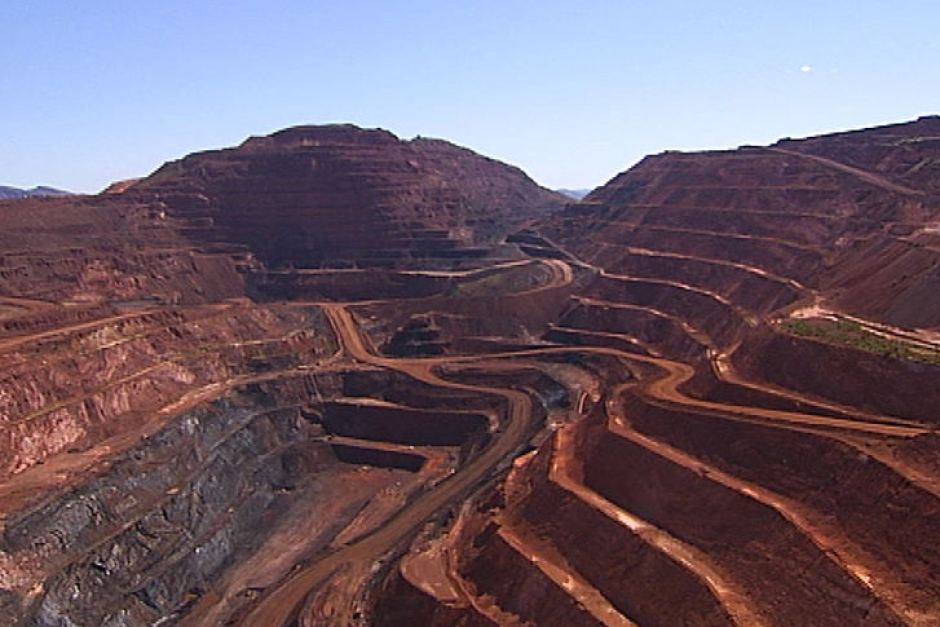
\includegraphics[width=12 cm]{ore-mine}
 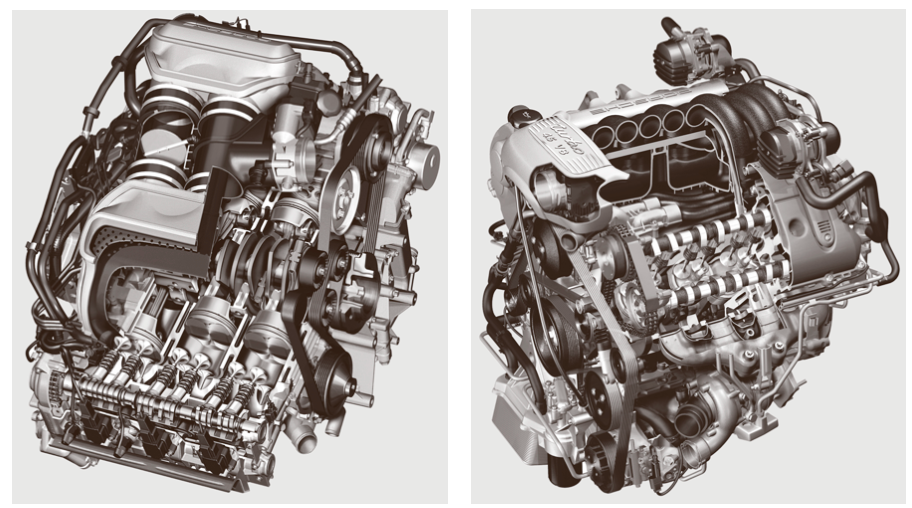
\includegraphics[width=12.5 cm]{car-engines}\end{center}
 % cc-trans.png: 1113x529 pixel, 72dpi, 39.26x18.66 cm, bb=0 0 1113 529
 \caption[Iron ore mine and 3D CAD images of two modern car engines]{
 Iron ore mine and 3D CAD images of two modern car engines. The iron
ore mine is located in Pilbara, western Australia (http://tinyurl.com/bde9y56).
The 3D CAD images are of two modern car engines. These 6 (left) and 8 (right)
cylinder Porsche engines may be larger than typical car engines, but are not
much more intricate, and share the same basic design as all modern internal
combustion engines for cars \citep[p.~1043]{grote2009springer}.}
 \label{f:car-engine}
\end{figure}
% This section should be in fundamentals!!!
Categorising and quantifying these processes is a difficult task.
The organisational supply chain that transforms
low quality (high entropy) natural resources into a
complex and highly accurate vehicle component such as an engine is long
and complex. Tracing the manufacturing processes, technologies and
material and energy consumption is even harder; this is the subject matter
of life cycle analysis (LCA), an academic field in its own right, with a
substantial branch dedicated to energy life cycle analysis \citep{kuemmel1997life,
cornelissen2002value}. It should come as little surprise, therefore that
``the literature shows a large variation in estimates of the energy needed to
manufacture a car (Moll, 1993)''
\citep[p.139]{Wee2000}.\footnote{The original 1993 dissertation, entitled
``Energy counts and materials matter in models for sustainable development,
dynamic life-cycle modelling as a tool for design and evaluation of long-term
environmental strategies'' is available on the University of Groningen's
website, but only as a scan of the introduction.
}
As with the energy
costs of fuel production, this is an uncertain science, and `best estimates'
from the literature must be used, combined with some common
sense and reason. Some estimates of the energy costs of cars are presented in
\cref{tcaren}. The range of methods and vehicles analysed is reflected in
the range of estimates: the highest (272 GJ) is more than \emph{three} times
larger than the smallest. At this stage the following dilema presents itself:
do we select the estimate that seems: Most authoritative? Most recent?
most related to the UK car fleet? Do we use this as the basis for best
and worst-case scenarios? Or do we take some kind of average?

Presented with these choices, it was decided to follow \citet{MacKay2009} and
place comprehensibility over accuracy: 100 GJ is a round number
that, to some degree, summarises the estimates presented in
\cref{tcaren}, and will be used as the central estimate of $EMv$.
This `rough estimate' is a deliberate
departure from previous work published by the author
\citep{Lovelace2011-assessing}, in which the most
`authoritative' figure was selected (the 272 GJ estimate used by the
authority figure, Professor David MacKay, so was assumed to be
`correct'). The reasons for selecting using the 100 GJ value is that the
variability in previous estimates suggests that the true value is
only really known to one significant figure. In place of using an
estimate that inspires confidence with its precision (e.g.~ 272 MJ),
this estimate acknowledges that the energy costs of car manufacture are highly
uncertain and variable over time, and require updating with more evidence. As
with the energy costs of fuel production, any estimate that is overly precise
risks being outdated very quickly.

To account for the fact that large cars require
more natural resources and hence energy to produce, 
\citet{Mikkola201023} assumed that embodied energy costs of manufacture
are roughly proportional to weight. Following this approach, the next stage is
to allocate the car categories that are provided in survey data (small, medium
and large) to average weights, and adjust the energy use estimate accordingly.
In fact, weight data on the UK car fleet was found to be elusive, especially
cross-tabulated with the 3-way categorisation of size used in the Understanding
Society and National Travel Survey datasets. The best source of information
on the weight bands of different cars that could be found was an appendix
of \emph{Cars Fit for Their Purpose}
\citep{plowden2008cars}.\footnote{Another
source of information considered was a joint
report by national transport research consultancies for the European Union
tackling the issue of safety \citep[appendix 2]{gail2006improver}.
They report the weights of 3 types of passenger vehicle specified by
the British Standard on crash tests, EN 1317-1:
825, 1300, and 1500. These last two values seem
representative compared with other figures,
but the first is far lower than cars in the supermini class.
}
Five categories of `conventional' cars, representative of the British car fleet,
were selected for comparison with
`eco cars': supermini, lower medium, upper medium, executive and multi-purpose
(4 X 4s and people carriers); with the follow weights: 1096,
1175, 1440, 1735, and 1674 kg. To match these to the
3 categories supplied by survey data, it is assumed that the `small' car
category corresponds to the supermini class. For the `medium' and `large'
categories, the average of lower medium and upper medium,
and the average of executive and multi purpose vehicles are taken respectively.
This results in the following weights: 1.1, 1.3 and 1.7 tonnes.
Thus, small and large cars are assumed
to be 15\% and 30\% lighter and heavier than the fleet average,
respectively.\footnote{These rounded values
were attained by using the medium-sized car weight
((1440 + 1175) / 2 = 1307.5)
as the denominator: 1096/1307.5 = 0.838 was rounded up
to 15\% lighter for simplicity; (1735 + 1674) / (1440 + 1175)
= 1.304.
}
Although these values are not considered to be
accurate,\footnote{The
definitions used to define small, medium and large cars
are not defined in terms of weight in the survey questionnaire,
precluding any hope of precision.
}
they do coincide with other weight figures
(e.g.~ those presented in \citep[appendix 2]{gail2006improver}, who quote an
average weight for the EU's fleet as 1376 kg.), reflecting the fact that
the weight distribution of cars is positively skewed and providing
intuitively easy to remember values providing no false sense of accuracy.
These average weights will be used to
adjust the 100 GJ $Ef_{car}$ value.

\begin{table}[h]
\caption{Estimates of the energy costs of car manufacture (EMv)}
\begin{center}
 \begin{tabular}{p{3cm}rrp{6cm}}
 \toprule
 Source	& EMv (GJ)	&MJ/kg	&Comments\\
  \midrule
\citet{burnham2006development}	&110	&	&Typical US car, assumes materials are recycled\\
\citet{MacLean1998}	&	&86.6	&Detailed, widely referenced study\\
\citet{Mikkola201023}		&81.2	&134&Data presented in MJ/kg from a large (1.6 tonne) car\\
\citet{Simonsen2011}	&85.56	&	&VW Golf (VW estimate)\\
\citet{sorensen2004total}	&87	&	&Toyota Camry\\
\citet{sorensen2004total}	&88	&	&VW Lupo, production and materials\\
\citet{sorensen2004total}	&178	&	&DaimlerChrysler F-Cell\\
\citet{Treloar2004}	&272	&	&Economic-based calculation, used in MacKay (2009)\\
\citet{Uson2011-eco-eff}	&114.3	&	&Used commercial life cycle analysis software\\
\bottomrule
 \end{tabular}\end{center}
 \label{tcaren}
\end{table}

% Similarly rough estimates have been used to characterise the energy costs
% of the manufacture of other vehicles although, as with cars, extensive literature
% searches were first conducted in order to inform and corroborate our estimates.
% As illustrated in \cref{tven}, our estimates acknowledge the uncertainties
% in current life cycle analyses and are justified with reference to the
% literature as well as intuition. % Removed as it adds little and contains
% reference to a table that does not exit!

No research directly tackling the energy costs of bus manufacture could be found.
However, an article looking at agricultural machinery approached the
problem by focussing on weight \citep{Mikkola201023}. The same approach is
taken here: it is assumed that the energy inputs per kilogram will be the same
for cars as for larger vehicles. From a
search of bus specifications, it was discovered that buses tend to weigh
a little more than 10 tonnes.\footnote{Alexender Dennis's
Enviro200, ``the world's \label{fnbuses}
most popular midi bus'' weighs 13.1 tonnes
(\href{http://www.alexander-dennis.com/uploads/files/e200_spec_sheet.pdf}
{alexander-dennis.com}); the Enviro300, also very common
in the UK, weighs 14.4 tonnes
(\href{https://en.wikipedia.org/wiki/Alexander_Dennis_Enviro300}{Wikipedia});
the double-decker Wrightbus NB4L, common in London, weighs 12.65 tonnes; the
Cummins engine 23-34 passengers inner city bus weights 12 tonnes.
At the top end of the range, the Alexender Dennis  Enviro35OH,
an electric-hybrid bus (i.e.~with additional weight due to batteries)
weighs 19 tonnes.
These weights were supported by a paper comparing the fuel use of three
`state of the art' buses \citep{pelkmans2001emissions}:
they each weighed between 11 and 14 tonnes. Incidentally, each of these
boasts new and improved fuel use, due in part to their light weight.
}
Inter-city coaches are heavier, due to their additional size (for seating capacity
and luggage space) and the fact they do not need to accelerate as
frequently as buses so are less dependent on
weight for fuel consumption: they were assumed to be on average 20
tonnes, or approximately 15 times the weight of a typical
car.\footnote{The Volvo 9700, for example, weighs 18 tonnes
(volvobuses.com).}
Based on these weights, the energy cost of coach and bus manufacture was
estimated to be $EMv_{car}$ multiplied by 10 and 15 respectively.

A similar logic was used to estimate the embodied energy of bicycles:
a typical bicycle weighs $\sim$12 kg, 100$^{th}$ the weight of an average
car so the energy costs of its manufacture are assumed to be 100 times less
as well.
% \footnote{This corroborates with pasts studies...} !!!
Similar techniques could be used to estimate the embedded energy costs of
trains, trams and even walking (due to the energy costs of new shoes).
However, given the relatively small proportion of trips made by these
`vehicles', coupled with the lack of evidence about their embodied energy
costs, $EMv$ was not calculated for these modes.

As Fels' formula (\cref{eq:esys}) shows, the average vehicle lifespan
($Lv$) is
needed to convert these embodied energy costs into costs per unit distance.
The best available estimates that could be found of 
$Lv$ were 150,000, 750,000 and 20,000 km for cars, buses and bicycles
respectively.
% \footnote{Definitely needed here!!!}


\subsection{Guideway manufacture} \index{energy use! road construction}
\index{roads}
Returning to the thought experiment conducted for vehicle manufacture, it
should be clear that it can be taken further. Imagine the car in isolation
from the rest of society: placed into the pre-industrial natural environment,
it would be of little use, even if petrol were available.
It is only with supporting infrastructure including roads and the flat,
compressed ground that they depend on, petrol stations, garages, bridges
etc.~that cars can move people. All of these objects require large one-off
energy inputs to be created, and continual energy inputs for maintenance. By
considering the natural environment next to the
man-made environment for cars, another, longer-term energy cost becomes clear:
without incessant energy inputs the built environment would tend to degrade,
gradually returning to its natural
state.\footnote{Post-collapse Soviet settlements
and parts of Europe most seriously affect by the post-2008 recession
(e.g.~Southern Spain)
illustrate this process well: tree roots eventually crack and rupture roads;
weeds overtake abandoned petrol stations and bridges eventually fail without
regular maintenance.
}
The concept of entropy may be helpful here: roads and other built objects
can be seen as having a lower level of entropy than their surroundings, an
imposition of straight edges and surfaces on a largely stochastic and fractal
landscape. Yet the second law of thermodynamics states that entropy always
increases in closed dynamic systems; this explains why motorised transport
infrastructure not only requires large energy inputs at the outset, but also
commits future generations to future inputs if they want them to work.

The above discussion makes it clear that road and rail construction is a
highly energy intensive activity. However, only one recent study could be
found that quantified the energy costs of road construction.
\citet{Treloar2004} conducted a very detailed `hybrid life-cycle analysis',
attempting to convert the full range of processes and materials
--- including the embodied energy contained in concrete, steel and cement, as
well as the processes of construction and financing needed to make the
contract happen --- into energy units. Eight estimates of embodied energy
were presented for eight different road types, ranging from `granular'
tracks (42 TJ for 5 km, with a lifespan of 20 years) to heavy duty
`full-depth asphalt' roads (195 TJ for 5 km, lifespan of 40 years).
For their main case study, of `continuously reinforced concrete' roads,
the energy costs of construction were found to be 136 TJ for a 5 km stretch
(27.2 GJ/m). Adding maintenance energy costs of 4\%  per year, the total
cost increased by a factor of 4.6. This is equivalent to 35,000 kWh/m
overall.\footnote{27.2 
$\times$ 4.6 = 125 GJ/m. 125 $\div$ 3.6 = 35 MWh/m.
}

\citet[p.~90]{MacKay2009} used these estimates as the basis of his estimates
of road energy costs in the UK, per person: ``Let’s turn this into a ballpark figure
for the energy cost of British roads. There are 28,000 miles of trunk roads
and class-1 roads in Britain (excluding motorways). Assuming 35,000 kWh
per metre per 40 years, those roads cost us 2 kWh/d per
person.''\footnote{This 
result was independently verified as follows:
35,000 $\div$ (40 $\times$ 365) = 2.40 kWh/m/d.
2.40 $\times$ (28,000 $\times$ 1.61 $\times$ 1000) m = 108,000,000 kWh/d.
108 $\div$ 60 million people = 1.8 kWh/p/d.
}
Given that roads are used for 500 billion pkm each year \citep{Mills2011},
this translates into
an average energy cost of $EMg_{road}$ = 0.3
MJ/pkm.\footnote{125000 MJ/km $\times$ (28000 * 1.61 * 1000) = 5.64 PJ for all
road transport over 40 years. 5.64 PJ divided by the number of pkms
travelled by UK citizens over that time (500 $\times$ 10\textasciicircum9 $\times$ 40)
provides this answer. The raw calculation using computer arithmetic in MJ,
is as follows:
(125000 * (28000 * 1.61 * 1000) ) / (500 * 10\textasciicircum9 * 40) = 0.282.
}

Of course, this value would vary greatly depending on a number of factors.
It is entirely feasible, for example, that larger cars cause more energy costs
due to road maintenance and that motorcycles cost less per pkm in terms of
road repairs. However, this estimate is so crude that adjusting it to account
for such factors (which appear not to have been sufficiently explored in the
LCA literature) would be presumptuous. As with the estimates of the
energy costs of fuel and car manufacture, round numbers are used to emphasise
our uncertainty in the result.

The availability of data required for the calculation of
$EMg$ for railways is even worse, so this value is applied to road-based modes
(which account for $\sim$98\% of commuting pkms) only.
The energy costs of bicycle lanes and footpaths would also be hard to
calculate and, in any case, would probably be negligible in comparison
with the energy costs of roads.

Of course, the values presented above vary from person to person and
over time and space, depending on a number of
factors. This `intra-mode' (within vehicles of the
same type) variability is the subject of the next three sections.

\section{Additional factors affecting energy use} \label{svariable}
% Or just additional factors
% This section should just get to the point: what are the numbers used,
% where they come from
Of the factors causing energy use in transport described in the first
section of this chapter, only the mode of travel has been analysed in
detail so far. Granted, mode of travel incorporates to some degree many
other factors such as mass, speed, acceleration and aero
dynamics\footnote{These,
in combination, help explain why the direct energy use of bicycles is
approximately 30 times less than that of cars per kilometre.} and the indirect
impacts of guideway and vehicle construction. However, there are a number of other
factors that are mostly or completely omitted by simple average values over
all annual passenger kilometres which are seldom included in estimates of
energy use \citep{Schipper1993}. Factors not yet considered, in rough
descending order of importance, include the following:\footnote{Other factors
could have been included on this list such as the diet of active travellers,
speed limits and demographics. These undoubtedly play a role, the scope of the
analysis is limited, to avoid trying to cover everything at
the risk of covering nothing in detail. Another important factor is
technological: recent and well-maintained vehicles tend to use less energy
than old and poorly maintained ones. This issue is partly covered (for cars)
in \cref{seffspace}.
}
\begin{itemize}
 \item Frequency of trip: the majority of this section assumes that distance
 is already known, and this is true a large extent on a per trip basis.
 However, cumulative distance travelled each year depends on how frequently
 the journey to work is made, including holidays. 
 \item Occupancy: full vehicles use less energy per pkm than empty ones.
 \item Trip distance: the average energy use per vkm varies greatly depending
 on the trip's distance: short trips tend to involve more frequent acceleration
 events per unit distance and therefore entail higher energy intensities.
 \item Circuity, a concept first encountered in \cref{Chapter2}, impacts on energy
 use directly when distances are estimated based on known Euclidean distances, and
 indirectly through the likelihood of twists and bends associated with circuitous
 routes.
 \item Traffic jams and general congestion are frequent in many settlements, and
 entail much higher energy intensities per pkm than the open road.
 \item Behaviour clearly affects the energy performance of vehicles, although
 measuring its impact is extremely difficult.
 \item Environmental conditions such as temperature, topography, road roughness
 and precipitation all affect vehicle energy use in a variety of ways.
\end{itemize}
It is the impact of these factors on energy use, and their implications
for the accuracy of our energy cost estimates over time and space, to which
our attention is now directed.
% 
% 
% \subsection{Sub-mode variations in efficiency}
% % tree graph of different modes
% 
% 
% 
% 
% %%% Not really sure what to do with this section - where does it fit?
% 
% % These will be returned to in the
% % evaluation of the results (Chapter x). % will they???!!!
% These factors can be classified as:
% \begin{itemize}
%  \item Technological: newer and smaller cars can are generally more efficient. The
% efficiency of cars, trams, trains, metro services and bicycles also vary, with
% newer designs often offering efficiency gains. Of these, variable fleet
% efficiencies of cars is the only one that will be quantified in this PhD.
%  \item Environmental: Transport in hilly areas will always require more energy per unit
% of horizontal distance. This is because the energy associated with moving mass
% against gravity is wasted on the downward slope (often as low grade heat
% generated through braking). It would be interesting to measure the impact of
% topographical and other (e.g. road surface) factors in transport efficiency, but
% this goes well beyond the scope of this PhD.
%  \item Behavioural: Efficiency is not merely a technological concept (Patterson 1996)⁠.
% The amount of energy used to get from A to B varies greatly depending on
% behaviour, whether you are on foot, cycling, or driving a car or public
% transport vehicle.
% \end{itemize}
% The nature of these factors vary from person to person,
% which helps explain the focus in this PhD on calculating energy costs
% at the individual level. Direct energy use is a function of distance
% travelled and mode; these are outputted at the individual level by the
% microsimulation model. These estimates are considered to be representative as
% they are constrained by census statistics. Re-aggregating the individual level
% data provides regional estimates of energy use. Thus, intra-mode variations
% in efficiency could theoretically be included using the spatial microsimulation
% method used in this PhD.
\subsection{Frequency of trip} \label{sfreq}
This chapter has, until now, made the implicit assumption that
travel to work distance is known, or can at least be estimated reliably based on
census statistics. This is indeed the case for estimates of usual one-way trip
distance, with a few exceptions. However, if the energy costs of travel to work
are to be compared with other energy uses, it is vital that they have the same
denominator: not energy use per trip to work, but something more common such as
energy use per year.

The translation of energy use per trip ($Etrp$) into energy use per ($ETyr$)
year is simple in theory:
\begin{equation}
 ETyr = ntrps \times Etrp
\end{equation}
where $ntrps$ is the number of return trips made to work each year. This number
clearly has a large effect on our estimates of annual energy use for commuting,
as it is directly proportional to $ETry$ so it is important that good estimates
are made.

On the individual level, the factors that affect
$ntrps$ are the type of job (part time or full time), holidays
(how many weeks per year multiplied by the number of trips usually made per week)
and days off sick or working from home. There is good data on each of these
variables (except duration of holidays) from the National Travel survey;
Understanding Society contains variables on number of hours worked
(an imperfect proxy for number of days) and whether the job is part or
full-time.\footnote{The variable
`a\_pjbptft' reports whether the current job is part-time or full-time;
`a\_jbhrs' reports the number of hours normally worked per week.
}
The number of trips made to
work and back each week can be extracted directly from the National Travel
Survey, counting the number of work trips made by individuals.
This information is plotted in \cref{fn-trips-hist}, which shows the distribution
of trip frequency by mode of travel to work.

\begin{figure}[h]
  \centerline{
    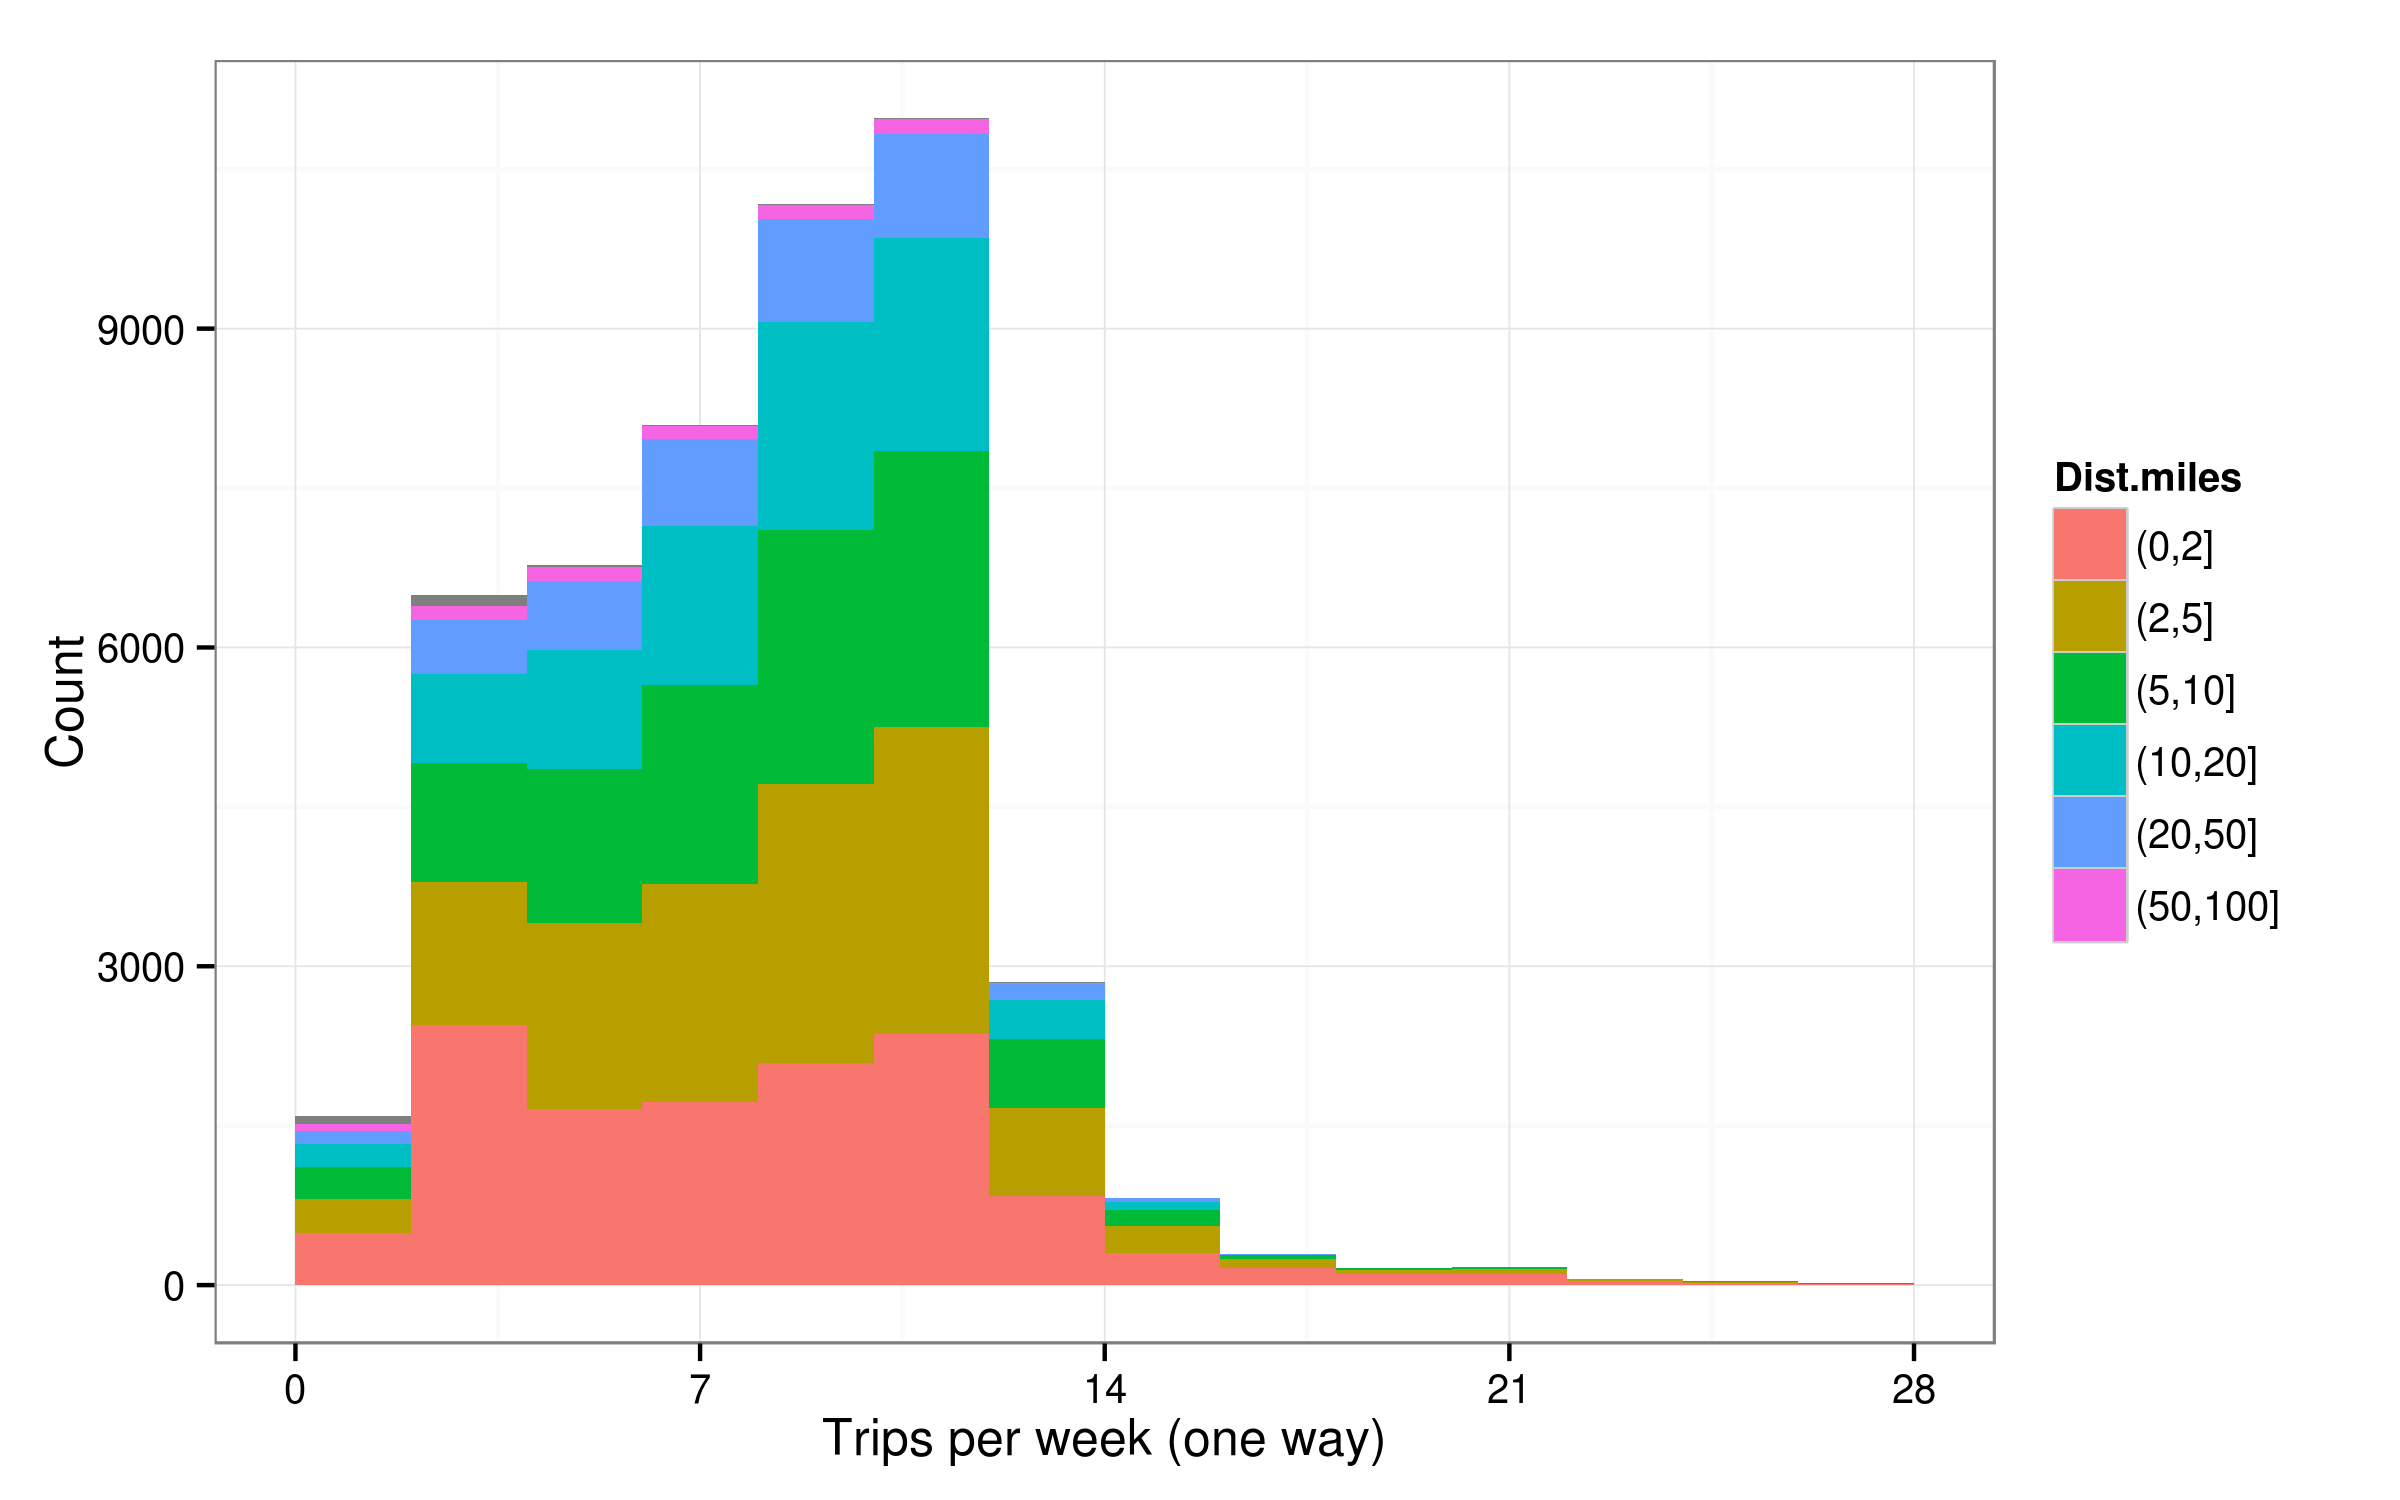
\includegraphics[width = 13 cm]{n-trips-hist}}
  \caption[Frequency of trips to work each week, by distance]
  {Frequency of one-way trips to work each week, by route distance (bin
  width = 2). Source:
  National Travel Survey 2002-2008.}
  \label{fn-trips-hist}
\end{figure}

The most common frequency of trip represented in \cref{fn-trips-hist} is 10
return trips per week, the standard for a 5 day working week, as would be
expected. However, people who make 9 to 11 trips per week (around 1/3 of
respondents, bizarrely, report travelling on one-way trips to work and back
an odd number of times) account for only 30\% of all commuters.
The average number of work trips made each week is actually substantially
lower, 7.3 per week, due largely to the influence of part time workers.
Based on this information, it could be assumed that this average value is
representative
of all commuters and applied to all individuals: it accounts both for the
effect of part time work, and the fact that many commuters work from home
some of the time (see \cref{ffreq-nts} in the previous chapter).
However, it is clear that
shorter trips are likely to be made more frequently than longer trips
(\cref{fn-trips-hist-prop}), which reduces the annual energy use estimates.
% The impact of this effect only becomes large for very frequent trips
% (which are dominated by short trips, presumably accounting for short shifts and
% trips home for lunch)
% so this effect was not included in the trip frequency estimates.
To take this effect into account at the individual level, a simple
regression model was run to find the relationship between average trip
distance and trip frequency, based on the information plotted in
\cref{fntripsdist}. It was found that the relationship was
approximately linear (despite the non-linear appearance
of \cref{fntripsdist}, due to varying bin sizes on the x axis),
and the following formula could account for the majority
(adjusted R-squared =  0.87) of the variation in
average trip frequencies:\footnote{The
R code to produce this result is available in the file
{\color{blue} \href{https://github.com/Robinlovelace/thesis-reproducible/blob/master/trip-plots.R}
{``trip-plots.R''}}
in the {\color{blue} \href{https://github.com/Robinlovelace/thesis-reproducible}
{thesis-reproducible}} Github repository.
}
\begin{equation}
 f = 7.9 - 0.023 dR
\end{equation}
where $dR$ is the route distance in km.
At the aggregate level, this information is more useful as a table of
bin-wide averages, calculated after converting miles into km and route distance into
Euclidean distance (\cref{tdistable}). For aggregate level calculations,
these frequencies can be multiplied by the number of people travelling
in each distance band, before multiplying by the number of working weeks
per year (assumed to be 44, account
for holidays and periods between jobs).

\begin{table}[htbp]
\caption{Average frequency of trips for Euclidean distance bins}
\centering{\begin{tabular}{lllllllll}
\toprule
D (km, Euclidean) & (0,2] & (2,5] & (5,10] & (10,20] & (20,30] & (30,40] & (40,60] & (60,200] \\
\midrule
F (trips/wk) & \multicolumn{1}{r}{7.2} & \multicolumn{1}{r}{7.6} & \multicolumn{1}{r}{7.4} & \multicolumn{1}{r}{7.3} & \multicolumn{1}{r}{7.0} & \multicolumn{1}{r}{6.9} & \multicolumn{1}{r}{6.5} & \multicolumn{1}{r}{4.3} \\
\bottomrule
\end{tabular}}
\label{tdistable}
\end{table}

\begin{figure}[h]
  \centerline{
    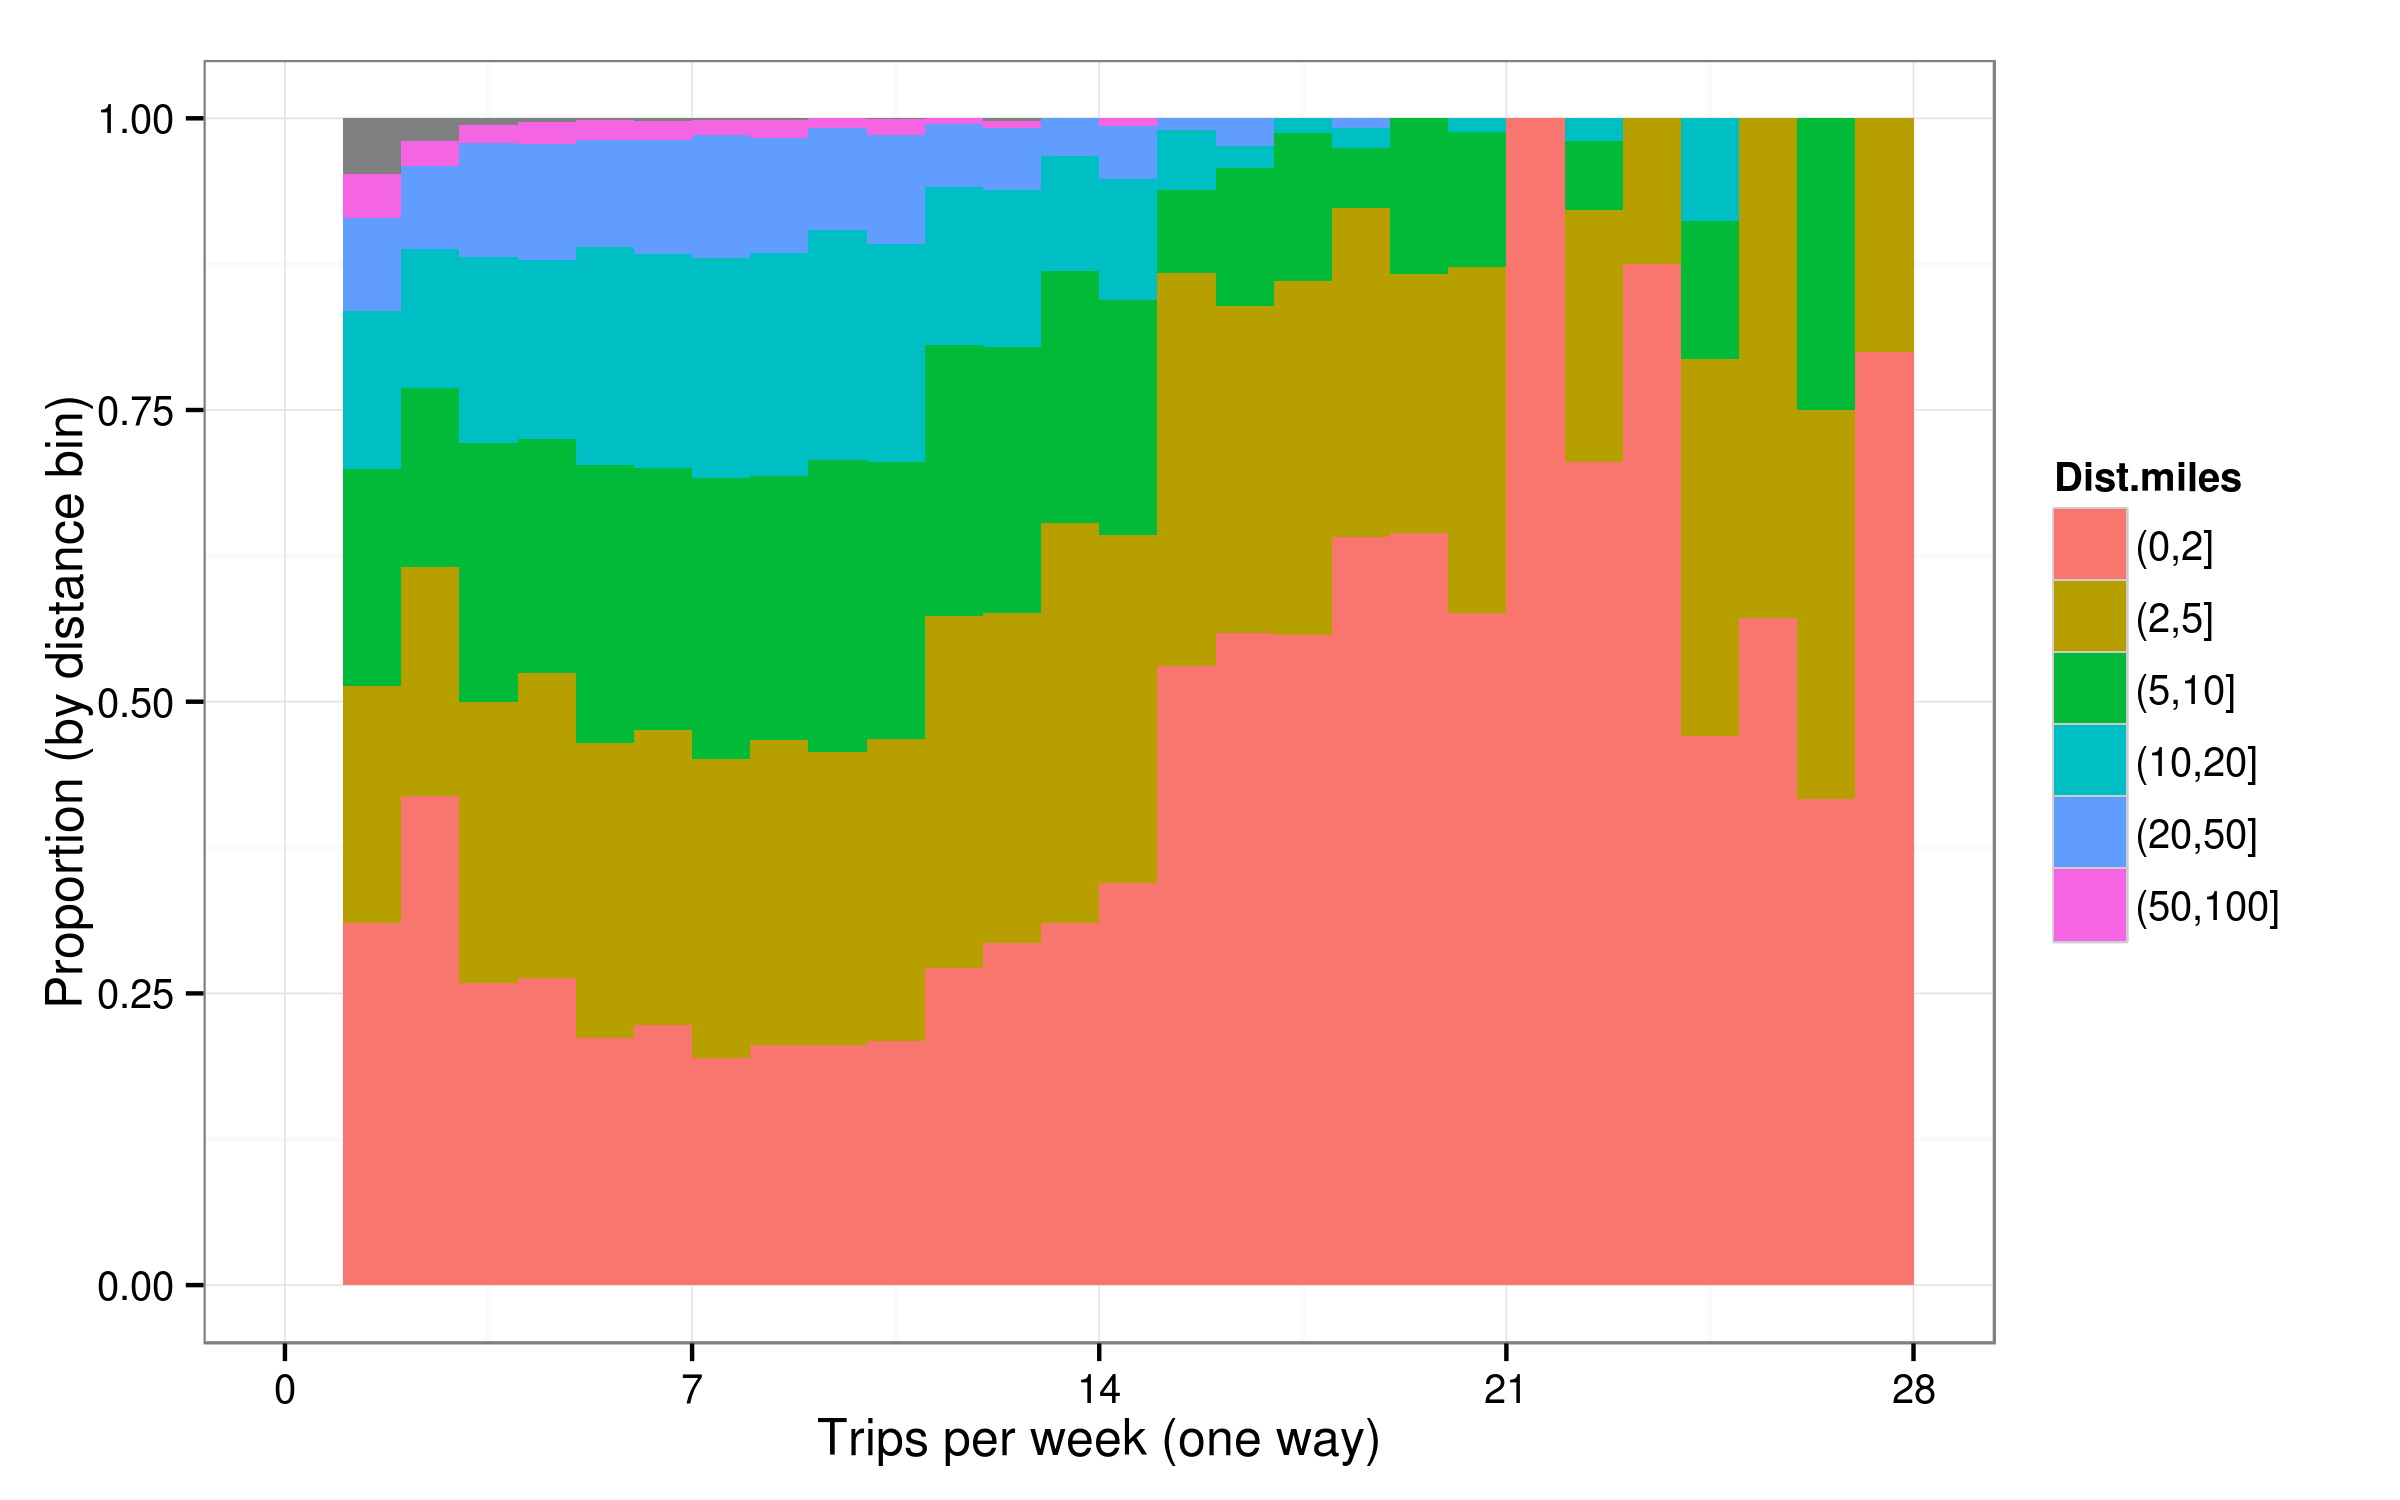
\includegraphics[width = 12 cm]{ntripshistprop}}
  \caption[Proportion of trips by distance for different trip frequencies]
  {Proportion of distance bands in for each frequency of one-way trips
  to work each week (bin  width = 1). Source:
  National Travel Survey 2002-2008.}
  \label{fn-trips-hist-prop}
\end{figure}

\begin{figure}[h]
  \centerline{
    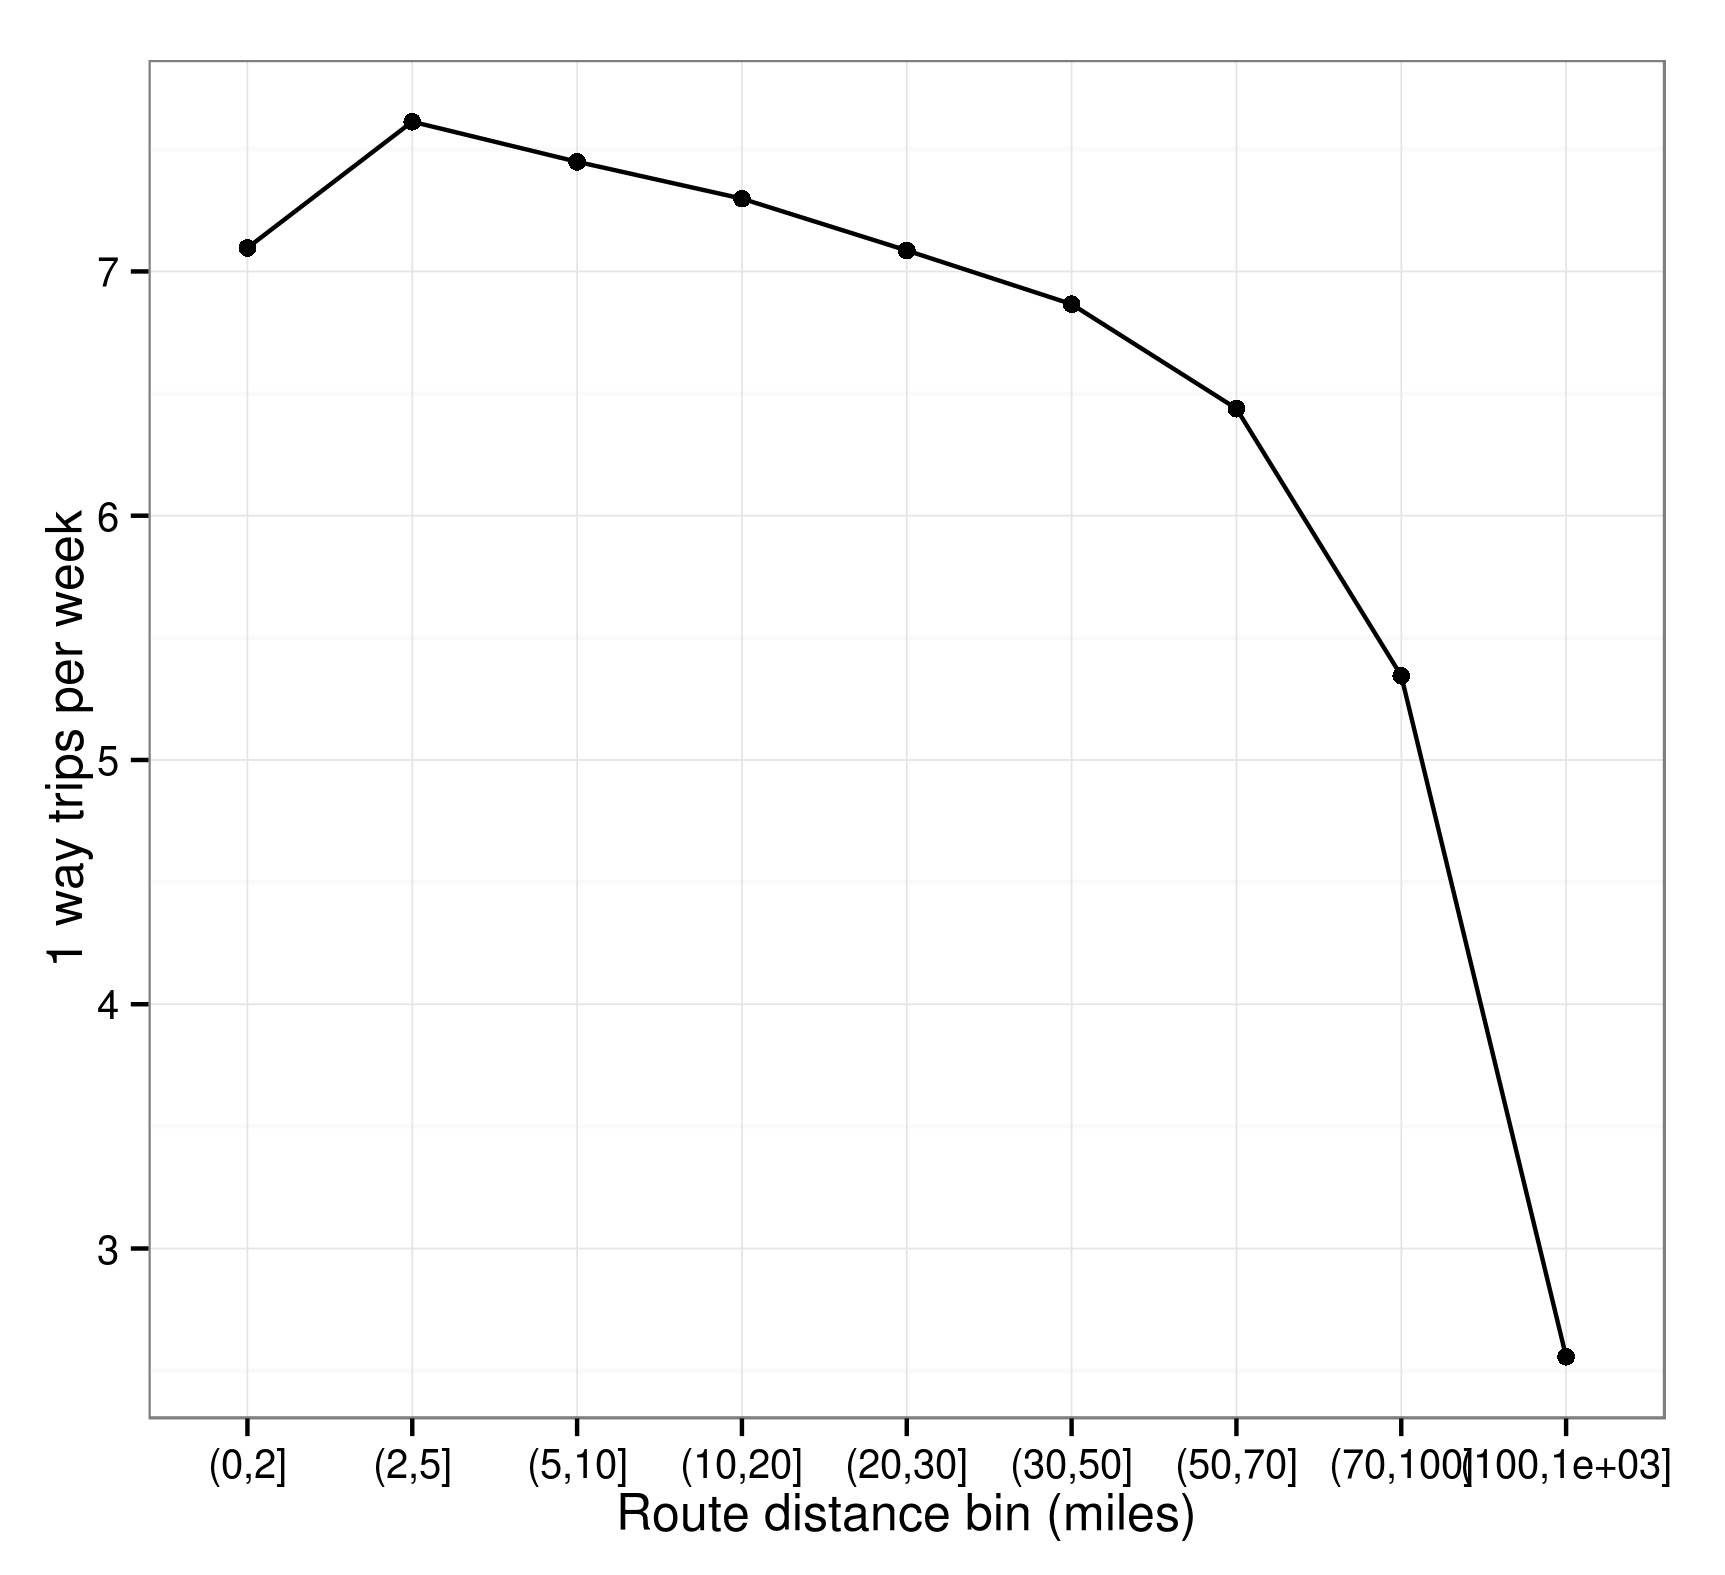
\includegraphics[width = 9 cm]{ntripsdist}}
  \caption[Relationship between trip frequency and distance]
  {Number of trips made to work per week as a function of distance. Source:
  National Travel Survey 2002-2008.}
  \label{fntripsdist}
\end{figure}

Another way of encapsulating these
factors, harnessing data that is available in the Understanding Society dataset,
is to express the number of trips made as a function of hours worked.
This makes sense for a number of reasons: it accounts for the fact that
`full-time-ness' and `part-time-ness' are not the binary categorical variables
that census data claim, but a continuum between working all day every day to
working a couple of hours per week. In addition, it harnesses information that
is available in the Understanding Society survey dataset (variable `a\_jbot'
hours worked per week) and produces more realistic distribution of
trips per year, that depend on social attributes,
than the single values per distance proposed above. (Also, one could
add a part-time/full-time constraint based on geographic census data,
although this has not been done).
The difficulty here is to account for holidays and variable shift
lengths.\footnote{20
hours worked per week, for example, could
imply 2 home-work trips for long 10 hour shifts or 4 journeys if each
shift is 5 hours long, the latter using double the energy of the former.
}
It was assumed that the average shift length was 6 hours, based on
``conventional working hours'' being 09:00--17:00 (8 hours)
\citep{harrington2001health}, combined with the knowledge that typical shifts
in hotels and restaurants are closer to 4 hours, and the fact that some people
travel home during lunchtimes or work half days during the weekend (each
factor making the working day shorter).
Further, it was assumed that 6 weeks of holiday were taken per year,
meaning 44 weeks of work per year.
This assumption follows a similar logic as that employed to estimate
the duration of an average working day: the mean number of weeks worked per
year by British adults is 47.5, but this number was reduced to account for
the fact that people change jobs (leaving a period of unemployment) and
do not always travel to work on `work days' due either to time off sick
or working from home.

To include these crude estimates into our estimates of annual energy costs,
the following R code was used.
\begin{lstlisting}[float=h, caption={Code used to
translate hours worked per week into number of trips per year}, label=ctrpyr]
# Assuming 8 hr days, 44 weeks/yr (8 holiday)
trips <- round(all[[i]]$a_jbhrs / 8 * 44  ,digits=0)
# Preventing people travelling to work more than 365 times/yr
trips[which(trips > 365)] <- 365
# Assuming part-time work or telecommuting (no response in survey)
 trips[which(trips < 10)] <- 100
\end{lstlisting}

Of course, these estimates of number of trips per year are not at all
accurate and therefore introduce a large amount of uncertainty into our
energy use estimates. For this reason, for the majority of the analysis
presented in the subsequent chapter, energy use is represented in units of
energy use per trip ($Etrp$). However, the ability to transfer these
estimates into energy use per year estimates proves useful when developing
metrics of vulnerability, or comparing the relative importance of
commuting with other energy-using activities. 

\subsection{Occupancy}
Occupancy ($Occ$) is defined as the number of people travelling in a vehicle, and
is often presented as an average value, aggregated over large expanses of time
and space. Although occupancy is already factored in to the energy-use
calculations mentioned above (and is implicit in census statistics for cars,
which discriminate between passengers and drivers) it can vary widely, with
large energy impacts.
Occupancy is roughly inversely proportional to energy use per person,
meaning that a single passenger in a car can halve its energy use per pkm
compared with the driver being the sole occupant, whereas a single additional
traveller on a bus containing 20 people will only result in a 5\% energy
saving.\footnote{These values
assume that no extra energy is required of the vehicle in question,
which is not strictly true. Assuming that energy use is proportional to
mass (in fact the relationship would be `sub-proportional' as extra weight
has no impact on air or rolling resistance, the other two critical forces
in driving), a 1.3 tonne car carrying an extra 80 kg of person and luggage would
use 6\% more energy, which is treated as negligible. The marginal
impact on a 12 tonne bus would be even less.
}

An alternative way of expressing occupancy is the concept of
\emph{load factor},\footnote{Some
authors have used the term `load factor' interchangeably with the concept
of occupancy (e.g.~\citealp{Jennings2013}), which could lead to confusion.}
\begin{equation}
 Lf = \frac{Occ_{average}}{Occ_{max}}
\end{equation}
the observed average occupancy divided by the mode's ``practical maximum''
\citep[p.~562]{Jackson1975} capacity under ideal conditions.
This metric is used primarily to standardise occupancy rates for public
transport modes (to account for the fact that maximum occupancy varies),
and has since been deployed to analyse energy use in public transport
\citep{Pisarski1975, Schafer1999}. Load factors have also been applied to
cars occasionally, resulting in the conclusion that empty seats
in cars represent a vast waste of resources \citep{Jackson1975}.
The main advantage of load factors, for all modes, is that they relate to the
vehicles \emph{potential} energy efficiency and its actual efficiency.
% This gap is greatest for cars, the occupancy rates of which we discuss first.

Based on both measures of occupancy, it is clear that small variations in
low occupancy modes can have
a relatively large impact on energy use, whereas small variations in public
transport occupancies will make of less of a difference overall. With this characteristic
in mind, this section proceeds to discuss car occupancy primarily before
tackling bus, rail and coach occupancy rates. 

The average occupancy of cars is reported at the national level and has tended
to decline over time in Britain, following trends in household occupancy,
although the rate of decline in occupancy rates is small compared
with those reported for the European Union as a whole and Ireland
(\cref{foccupancy}). Car occupancy also varies substantially depending
on reason for trip, as shown in \cref{toccupancy}. In fact, commuting is
the type of trip associated with the lowest rate of occupancy (1.2) and highest
proportion of single-occupant journeys (86\% of car trips to work contain
only a single person), joint with
business travel. The historical fall in occupancy rates, combined with
the very low rates of car sharing for the trip to work suggest there is much
room for improvement here.

\begin{figure}[h]
  \centerline{
    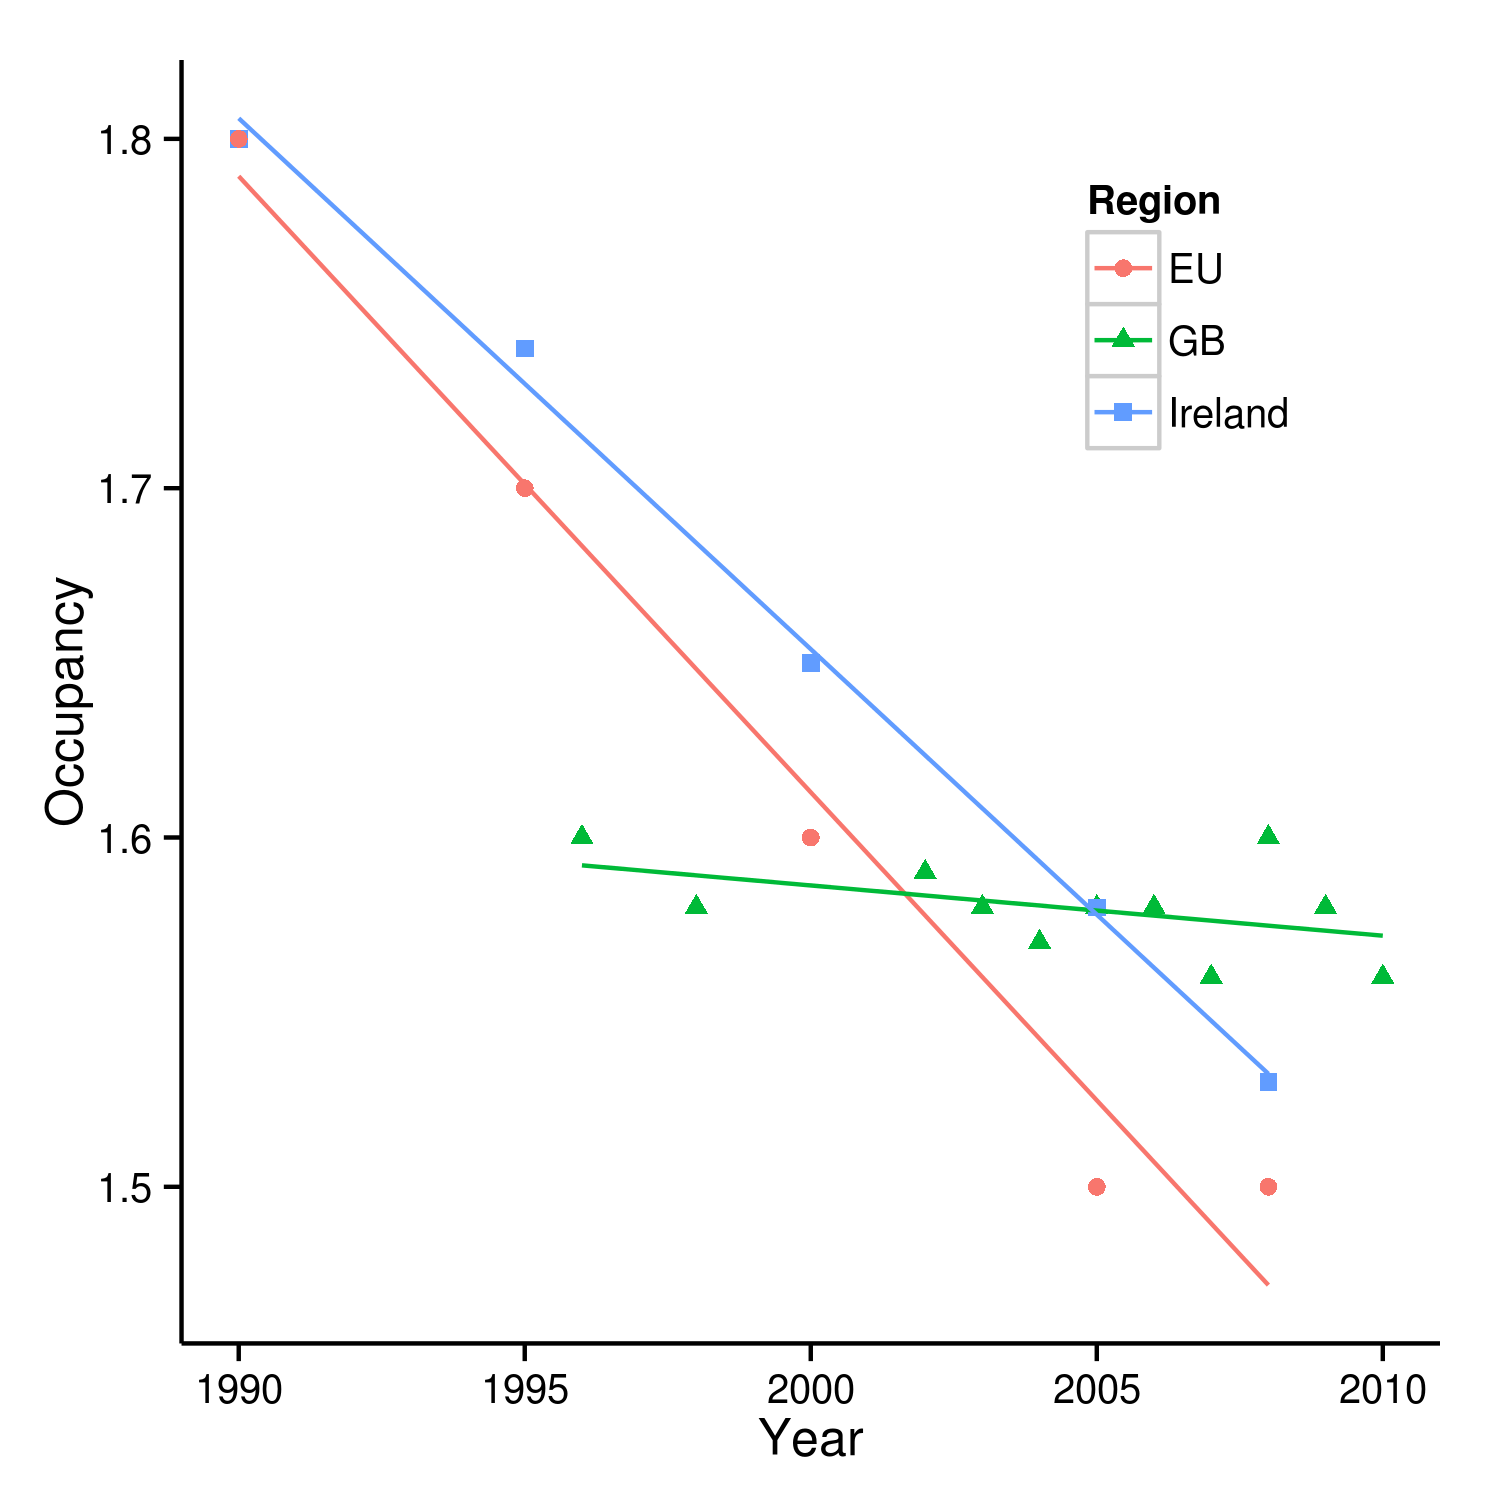
\includegraphics[width = 13 cm]{carocc}}
  \caption[Average car occupancies over time in three regions]
  {Average car occupancies over time in three regions.
  GB data from \citet[table 0905]{NationalTravelStatistics2012},
  EU and Ireland data from \citep{Jennings2013}.}
  \label{foccupancy}
\end{figure}

\begin{table}[htbp]
\caption[Average occupancy of car journeys by reason for trip]
{Average occupancy of car journeys by reason for trip.
Data from \citet[table 0906]{NationalTravelStatistics2012}.}
\begin{center}
\begin{tabular}{lrr}
\toprule
{Purpose} & Average occupancy & Single occupancy rate \\ \midrule
Commuting & 1.2 & 86 \\
Business & 1.2 & 86 \\
Education & 2.0 & 36 \\
Shopping & 1.7 & 50 \\
Personal business & 1.4 & 68 \\
Leisure2 & 1.7 & 53 \\
Holiday/day trip & 2.0 & 40 \\
Other including just walk & 2.0 & 35 \\
Total & 1.6 & 61 \\
\bottomrule
\end{tabular}\end{center}
\label{toccupancy}
\end{table}

In terms of our energy calculations, these statistics make little difference.
That is because the Census sensibly treats driving to work separately from
taking a lift in someone else's car. Therefore, the energy savings of
car sharing show up as a result of fewer people driving or travelling by
other forms of transport. The alternative would be to merge ``car driver''
($car.d$) and ``car passenger'' ($car.p$) into the single category of
the car, and set its average
energy costs as follows:
\begin{equation}
 Ef_{car} = \frac{car.d}{Occ_{car}}
\end{equation}

This option adds extra complexity to the energy use calculations,
however, hence our reporting of car drivers and passengers as different modes.
This approach also allows for the calculation of the occupancy rate of
commuter car trips in different areas:
\begin{equation}
 Occ = 1 + \frac{car.p}{car.d}
\end{equation}
This formula, used in conjunction with origin-destination flow data by mode,
could be useful for identifying areas in which could benefit most from
car sharing schemes.

\subsection{Efficiency impacts of trip distance}
The European Union certified test cycle involves two separate tests of energy
and emissions performance for different driving scenarios. This, and the
combined fuel economy measure that results, reflect the understanding that
more energy is used per unit distance during short trips (which predominate in
urban areas) than during long trips (generally inter-city). It would therefore
seem sensible to refine the estimates of $Ef$
presented in \cref{tdefra2} by the disaggregating them based on trip
distance. If most car trips are short, for example, our overall estimate could
be optimistically low.

Some research has been conducted in this area, although there seems to be a
 reluctance to make generalised statements about the relationship between
distance and fuel economy for different modes. This is because, as with so many
things in transport systems, the results will be context-dependent. In areas
where long-distance car trips are associated with very high speeds (e.g. between
two towns connected by an unregulated fast-flowing motorway), the fuel economy
could in fact rise above the average because energy use per unit distance rises
rapidly above around $\sim 90 kph$
(\cref{f:speeding-car}). As a general trend, however, short car trips
tend to be less fuel economical due to the stop-start nature of urban traffic
\citep{Anas2012-price-gas}.

\begin{figure}[h]
  \centerline{
    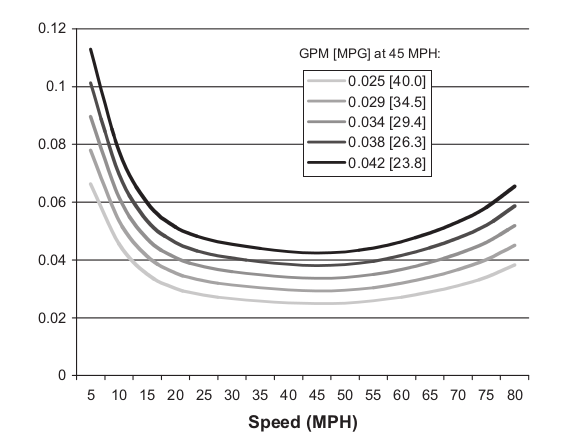
\includegraphics[width = 13 cm]{fuelec1997}}
  \caption{The impact of car speed on efficiency, from
\citep{Anas2012-price-gas}.}
  \label{f:speeding-car}
\end{figure}

The best multi-mode quantitative evidence that could be found on the matter was
\citep{bouwman2000tracking}. Using a micro level model written in
Matlab, simulated data recording the impacts of infrastructure, congestion,
and vehicle fleet on total energy use across 8 modes, as part of a PhD thesis
\citep{bouwman2000tracking}. The results, which are
normalised (by dividing the values by the all-distance average for each mode)
for a clear visualisation of how the issue affects each
mode differently, are presented in \cref{f:mirjan}. Bouwman's
\citeyear{bouwman2000tracking} model results in relatively small
shifts in fuel use as distance increases, declining by only 10\% between the
shortest trips and the least efficient trip distance, which was deemed to be 10
to 20 km. The calculations made in the model are not described in sufficient
detail Bouwman's thesis to comment on the likely reliability of the results, and
could not be accessed elsewhere. An additional problem with these estimates is
that they were developed for the Dutch transport system specifically, so may
not be applicable to the UK, even if there were high confidence in
the estimates. Therefore, taking these issues into account, it was decided not
to include Bouwman's (2000) estimates in the final
energy cost calculations: better evidence is needed on the matter.

\begin{figure}[h]
  \centerline{
    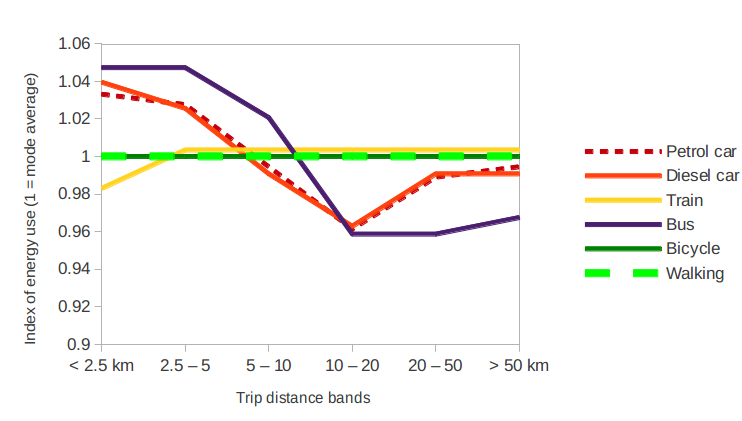
\includegraphics[width = 15 cm]{Mirjan-distance-ei}}
    \rule{35em}{0.5pt}
  \caption[Line graph of energy intensity vs trip distance]
  {Line graph of energy intensity vs trip distance. Data from
\citet{bouwman2000tracking}.}
  \label{f:mirjan}
\end{figure}

In the event of discovering better national (or even localised) estimates of
the relationship between distance and average energy usage, the method of
calculation is ready to accept these values.
% the energy use estimates presented
% in \cref{Chapter6} are calculated by Census distance bands (0-2 km, 2-5 km
% etc.) so it would be straightforward to weight these values based on the
% impact of distance on average efficiency in bands.

\subsection{Circuity} \label{scircuity} \index{circuity} \index{Euclidean
distance} \index{route distance}
In practice, the
network of roads, paths and other guideways of the transport system
rarely lead from a to b (or rather
i to j, in our notation) directly. Instead they
form a more or less circuitous path (\cref{fig:routes}). Previous work on this has
been conducted with respect to transport to work. There is strong empirical
evidence that circuity ($Q$) is \emph{not} constant, but varies depending on
the length of trip \citep{Levinson2009} and the structure of the transport
network \citep{parthasarathi2012network}, which varies between countries
\citep{Ballou2002} and continuously over space \citep{Barthelemy2011}.

\begin{figure}[h]
 \centering
 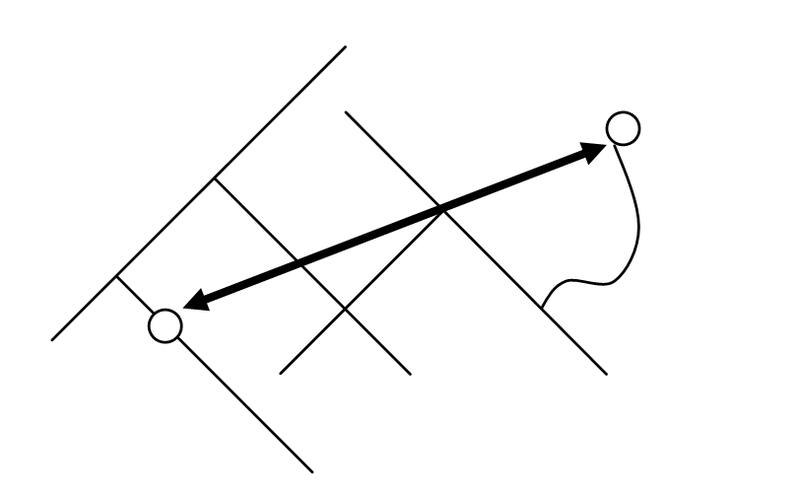
\includegraphics[width=7 cm]{EuclideanDistance}
  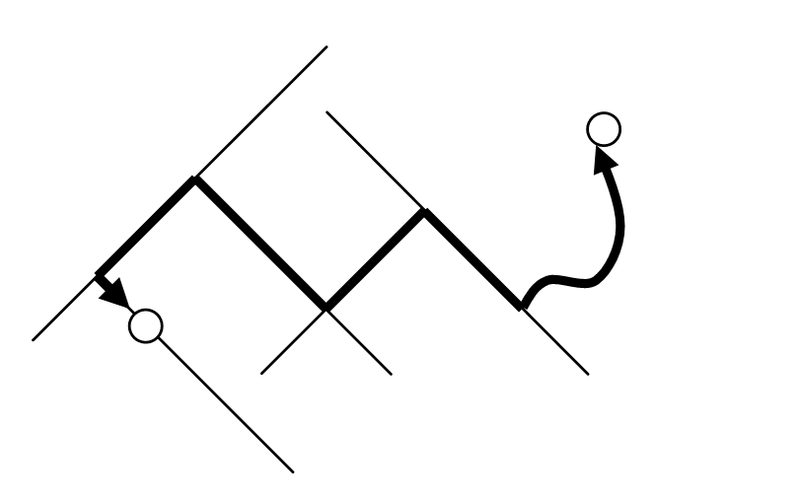
\includegraphics[width=7 cm]{NetworkDistance}
 \caption[Schematic of Euclidean and network distances]{Schematic of
 Euclidean and network distances. Thanks to David Levinson, who licensed this
 work, originally published in \citet{Levinson2009} with a Creative Commons licence.}
 \label{fig:routes}
\end{figure}

Regarding
typical values, $Q$ values between 1.21 and 1.23 have been reported for
walking trips to rail stations in Calgary, Canada \citep{O'Sullivan1996}.
\citet{Levinson2009} analysed the circuity of 5,000 home-work trips in and
around Portland, USA, and found an average circuity of 1.18 overall. In the
same study, it was also confirmed that
circuity is highly dependent on the distance travelled: for 50,000 random
point-pairs, circuity decreased from 1.58 to 1.2 as the distance increased from
5 km and less to over 45 km. Based on these results, a preliminary analysis
suggests that the relationship is logarithmic (\cref{fig:circuity}). In
the UK specifically, typical values of circuity were found to be
1.2 to 1.6 in a 1968 textbook \citep{bosco2012circs},
although the reliability and
coverage of this estimate is
questionable.\footnote{This estimate
was published over 40 years ago by \citet{cole1968quantitative},
``with the calculations done by having
students trace roadways on paper maps'' \citep[189]{bosco2012circs}.
The original is not cited in the quote because a hard copy of the book
could not be found. Therefore the quotation, from \citet{bosco2012circs}
is used.
}
\citet{Ballou2002} found an average circuity of 1.4 for England
as a whole, based on a sample of 37 points. Other than \citet{Levinson2009},
none of these studies
included the impact of distance on average circuity
values, instead reporting single values for entire areas.
\citet{Levinson2009} provide strong evidence to suggest that
circuity, taken as an average value over hundreds of measurements,
actually declines with distance, in a way that would be compatible
with all the previously mentioned estimates of circuity.

\begin{figure}[h]
 \centering
 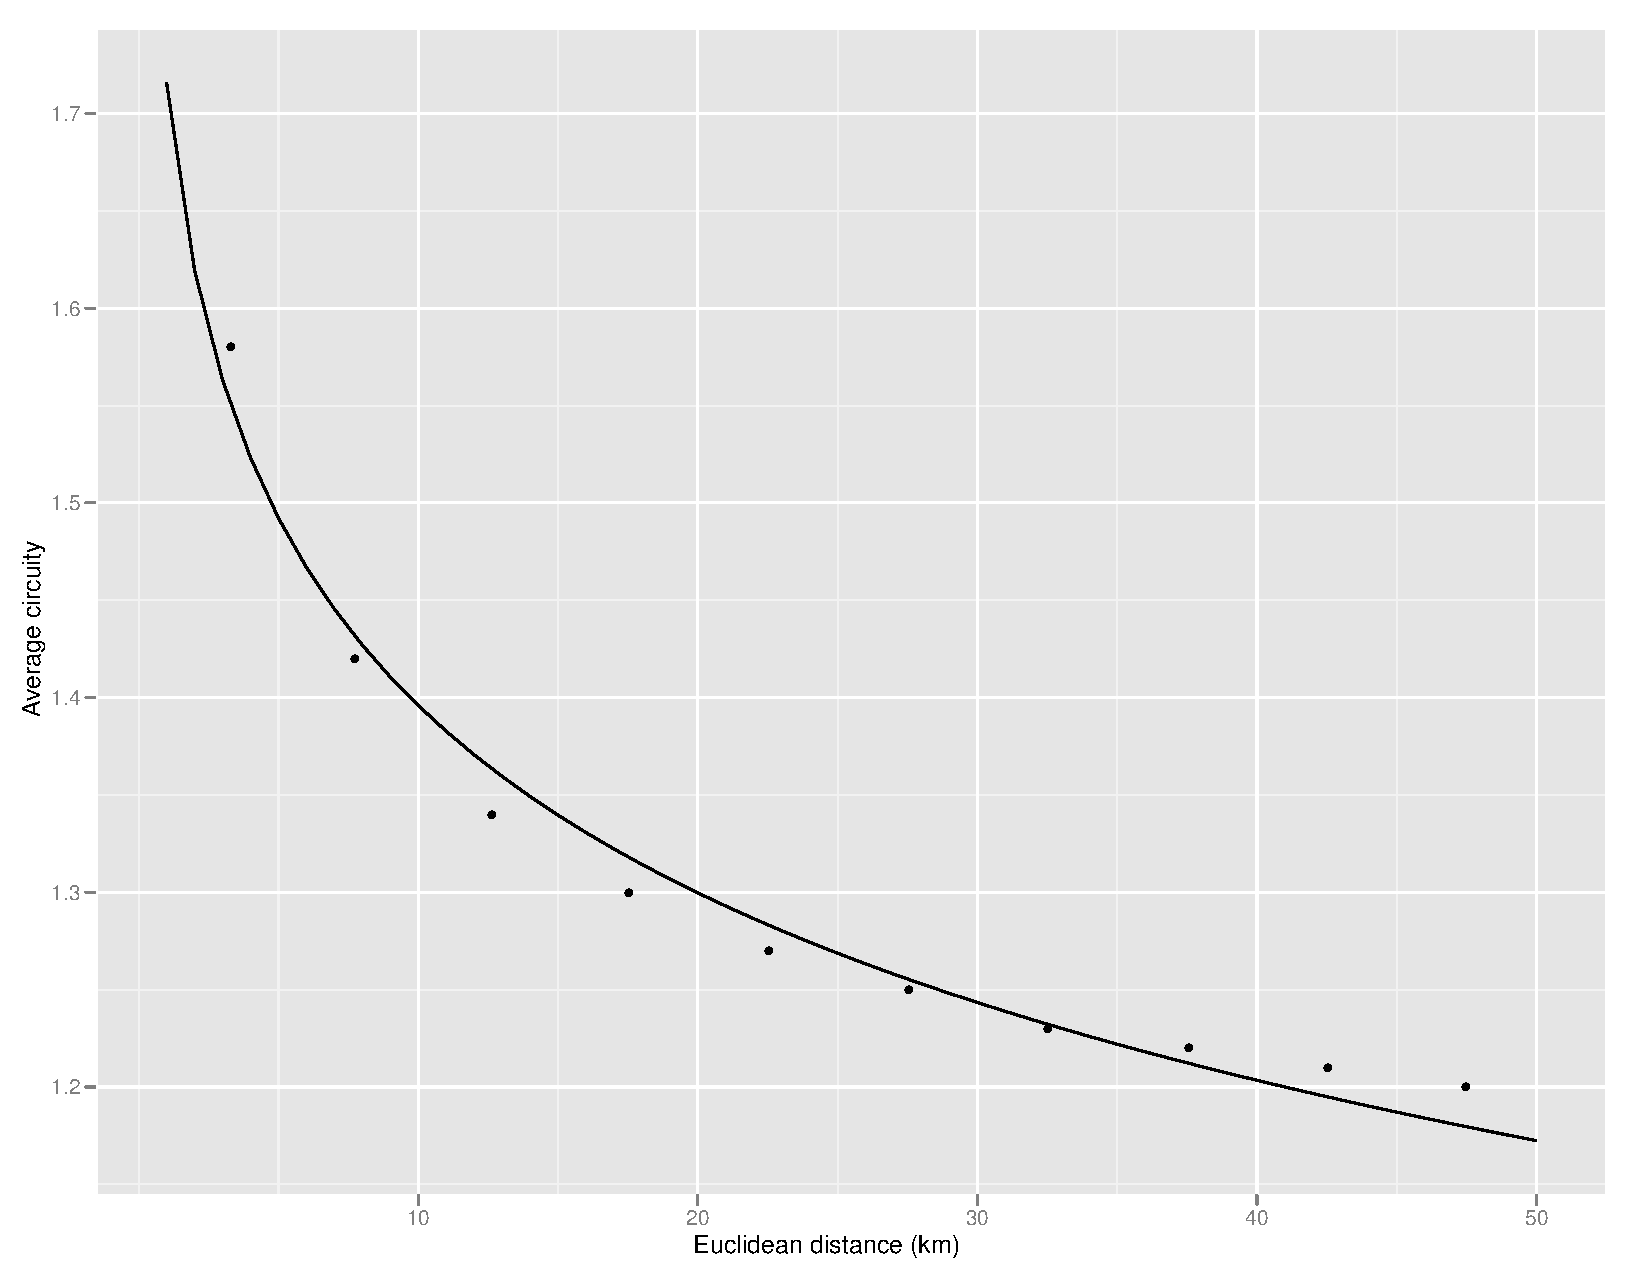
\includegraphics[width=14 cm]{circuity.pdf}
 % circuity.png: 550x450 pixel, 72dpi, 19.40x15.88 cm, bb=
 \caption[The decay of circuity with distance travelled]{The decay of circuity
with distance travelled. Data from
\citep{Levinson2009}, plotted here with a logarithmic decay ($y = a +
b*log(x)$), where $a$ = 1.72 and $b$ = -0.14. Coefficients calculated using the
command nls in R.}
 \label{fig:circuity}
\end{figure}

Analysis of the results from \citet{Levinson2009} suggest that $Q$ decays
logarithmically with increasing distance (see \cref{fig:circuity}):
\begin{equation}
Q = a + b \times log(dE)
\label{eq:circ}
\end{equation}
where a and b are coefficients calculated to be 1.72 and -0.14, respectively,
based on the \citet{Levinson2009} paper. Of course, using the results of
a US study as the basis for assumptions in the UK is no guarantee that the
assumptions will hold in practice, especially when
$Q$ varies from country to country (and almost certainly at lower levels also,
depending on the local road network and proximity of impassable obstacles
such as rivers, railways and motorways). There is additional support
for $Q$ decaying with increasing $dE$ from 
theoretical sources \citep{Barthelemy2011}.
The evidence reviewed suggests that, if one must
assume that $dR = f(dE)$ (as is the case here, as only Euclidean distances are
provided in the census data), \cref{eq:circ} is likely to
provide a more accurate description of reality than assuming that $dR = dE$.
The principle of Occam's razor states that the simplest solution that
fits the data should generally be preferred. In this case
recent evidence shows that $dR = dE$ simply
does not fit the data, so $Q = 1.7 + -0.14 \times log(dE)$
is used here. If a single circuity factor is required, Ballou's (2002) estimate
of 1.4 for the UK is recommended, especially as this coincides
with the circuity value interpolated in \cref{fig:circuity} around the 10 km
mark, roughly the median distance travelled to work in the UK.

Of course, circuity is affected by many other variables in addition to
Euclidean distance. In addition, it is wrong to assume that
more circuitous paths are always more energy intensive, as a complex
range of factors combine to determine the most energy efficient path
to take at any particular time \citep{Ericsson2006}. There are also large
inter-modal variations in circuity: pedestrians
and cyclists have been found to have particularly low $Q$ values \citep{Iacono2010}.
It can be expected that public transport users must endure longer route lengths
due to the need to get to and from train stations, bus stops and other
nodes to join the network, whereas cars and cycles can join almost anywhere.
In addition, it would be possible to weight $Q$ area by area, based on local
estimates of \emph{global accessibility} (see \cref{skeyconcepts})
that can could be computed by calculating the difference between $dR$ and
$dE$ for randomly (or intelligently) selected origin-destination pairs.

Beneficial as this process would be, yet these factors still omit
the impact of car park proximity, car sharing,
and multi-mode trips: in a more complex (potentially agent-based) model these
could conceivably be included.
For the time being it is assumed that \cref{eq:circ} holds for
all trips of the same distance: quantitative evidence of the impact of other
factors is scarce. If more data to weight $Q$ by other factors such
as mode emerges, the model should be updated.

\subsection{Efficiency impacts of congestion}
% As described in \cref{sdirecte}, the main official and publicly available
% source of information about fuel use is the EU's driving cycle test.
% As with much else in this chapter, these figures should not be accepted as face value.
% and real world values have been found to deviate substantially from their
% findings for many vehicles. To better evaluate the usefulness of the EU test
% data, we will explore the emissions testing process. The procedure for the
% urban part of the test is illustrated in \cref{f:testcycle}.
%%!!! Re-instate this at a later date!!!

The increased energy use of inner city driving compared with the rarely
realised (but frequently advertised) ideal of driving on open roads is
well established.
It is a result of far higher frequencies of acceleration/deceleration
events, due to the increased number of obstacles (e.g.~traffic lights) on
urban roads and the stop-start nature of congested traffic.
The impacts of this are reflected in the European Union's test cycle
requirements, that are used as the basis of CO$_{2}$ and fuel consumption
values that must be displayed by law on all car adverts (\cref{f:testcycle}):
two efficiencies are calculated --- urban and extra-urban. According to
\citet{Pelkmans2006}, urban driving uses around 30\% more energy per unit distance
than extra-urban driving in a Skoda Octavia TDi. Another paper reporting
real-world tests found that ``fuel consumption was about two times higher
[in city traffic] than for ring roads, which generally gave the lowest values''
\citep[p.~4649]{Vlieger2000}.

\begin{figure}[h]
  \centerline{
    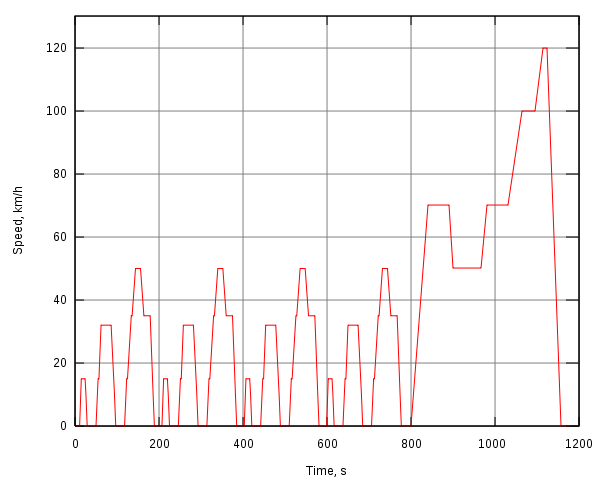
\includegraphics[width = 13 cm]{testcycle}}
  \caption[EU test cycle]{EU test cycle. Up to the 800 second mark,
  the car is in the `urban' part of the test. Beyond that point,
  the `extra-urban' stage begins.(This test cycle design explains
  why car adverts contain 2 or 3 mileage values.)}
  \label{f:testcycle}
\end{figure}

Part of the difference between the increased energy use of city driving
reported in  \citet{Pelkmans2006} and \citet{Vlieger2000}
is illustrated in \cref{fcarplot-urb}, which shows that the
difference between inner
city and rural driving is not constant across all cars. Of the randomly
selected sample of models plotted, the extra energy use of driving in
cities is on average 78\% higher than the average energy costs of driving
in the countryside, as measured by the (imperfect) European test
cycles (\cref{f:testcycle}). The efficiency impact ranges from a
34\% increase for the
Citroen C4 to more than double the energy use for the heavier
Audi A6 and Ford Mondeo models.

\begin{figure}[h]
  \centerline{
    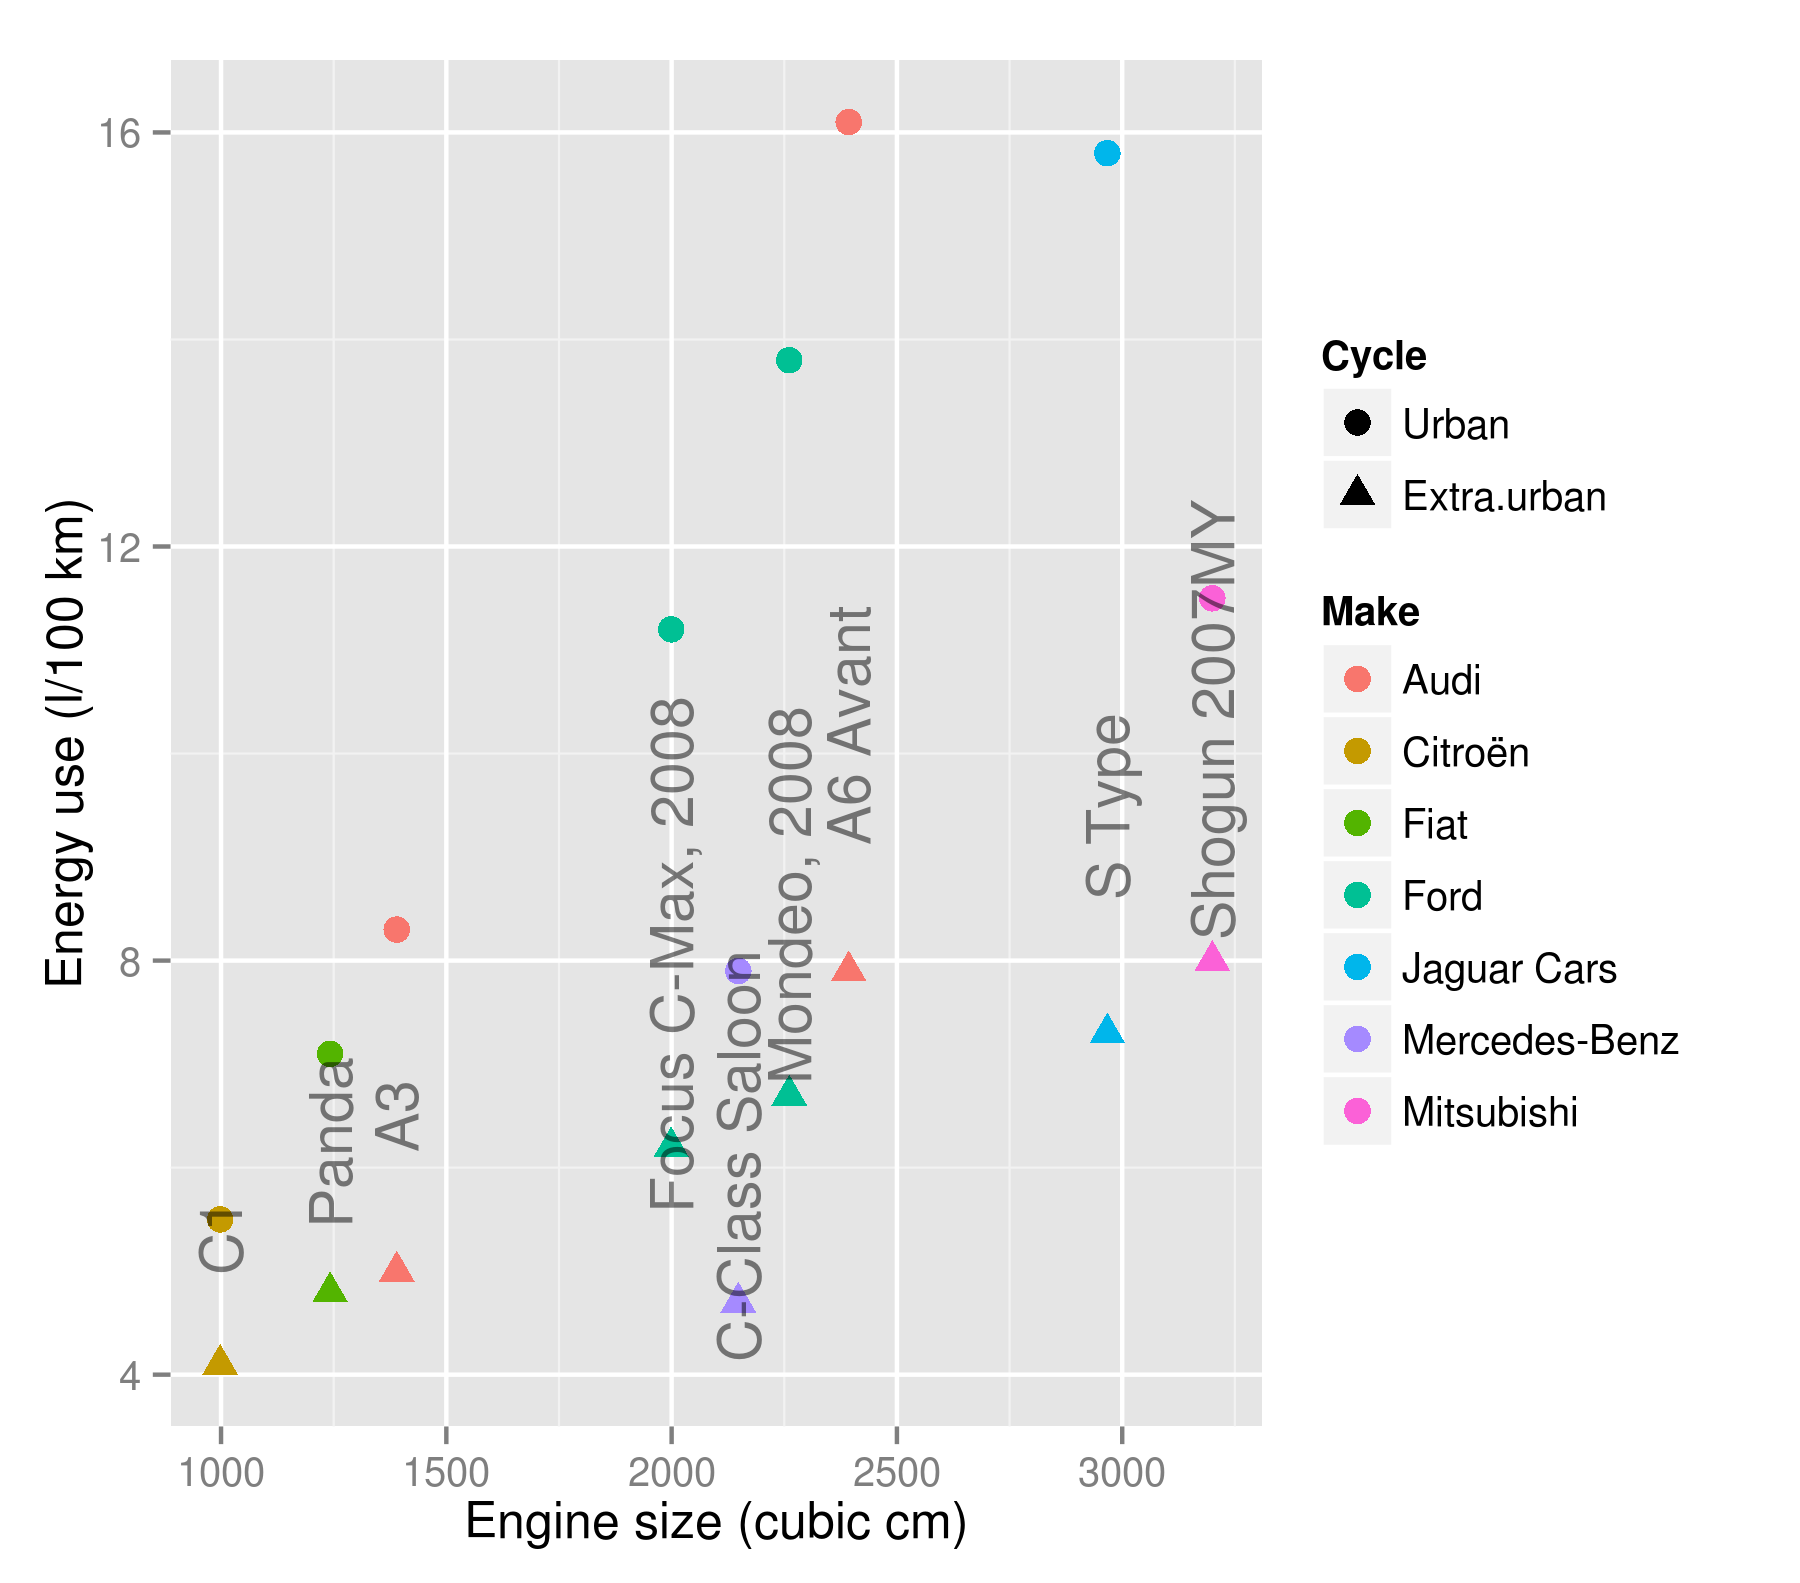
\includegraphics[width = 13 cm]{carplot-urb}}
  \caption[Urban and extra-urban energy use of selected models]
  {Urban and extra-urban energy use of selected models.
  Data from \href{http://www.vcacarfueldata.org.uk/downloads/latest.asp}
  {the Vehicle Certification Association}.}
  \label{fcarplot-urb}
\end{figure}

Because of this variability, and the fact that it is not known which models
predominate in different areas, it was decided not to include the
energy impacts of city driving into the model.
(It would have been possible to simply double the energy use for
short trips in urban areas, but it was felt that there is not sufficient
evidence for this additional layer of complexity in the energy
efficiency calculations at this stage.)
In any case, the energy impacts of congestion and city driving
more generally undoubtedly has a very large impact on energy use for personal
transport overall and commuting in particular, so attempts to quantify the effect
should be included in future work. The reason why commuting trips are
more likely to suffer from the effects of traffic jams than other
types of trips is illustrated in \cref{frushhour} and can be summarised
in two words: rush hour. The timing of commuter trips could therefore be
an additional factor influencing overall energy use estimates. No attempt to
quantify this effect is made here, however: there is no geographical data on
the timings of commuter trips. Rush hour traffic is the culmination of many
individual decisions. As shown below, these behavioural factors are difficult
to quantify.

\begin{figure}[h]
  \centerline{
    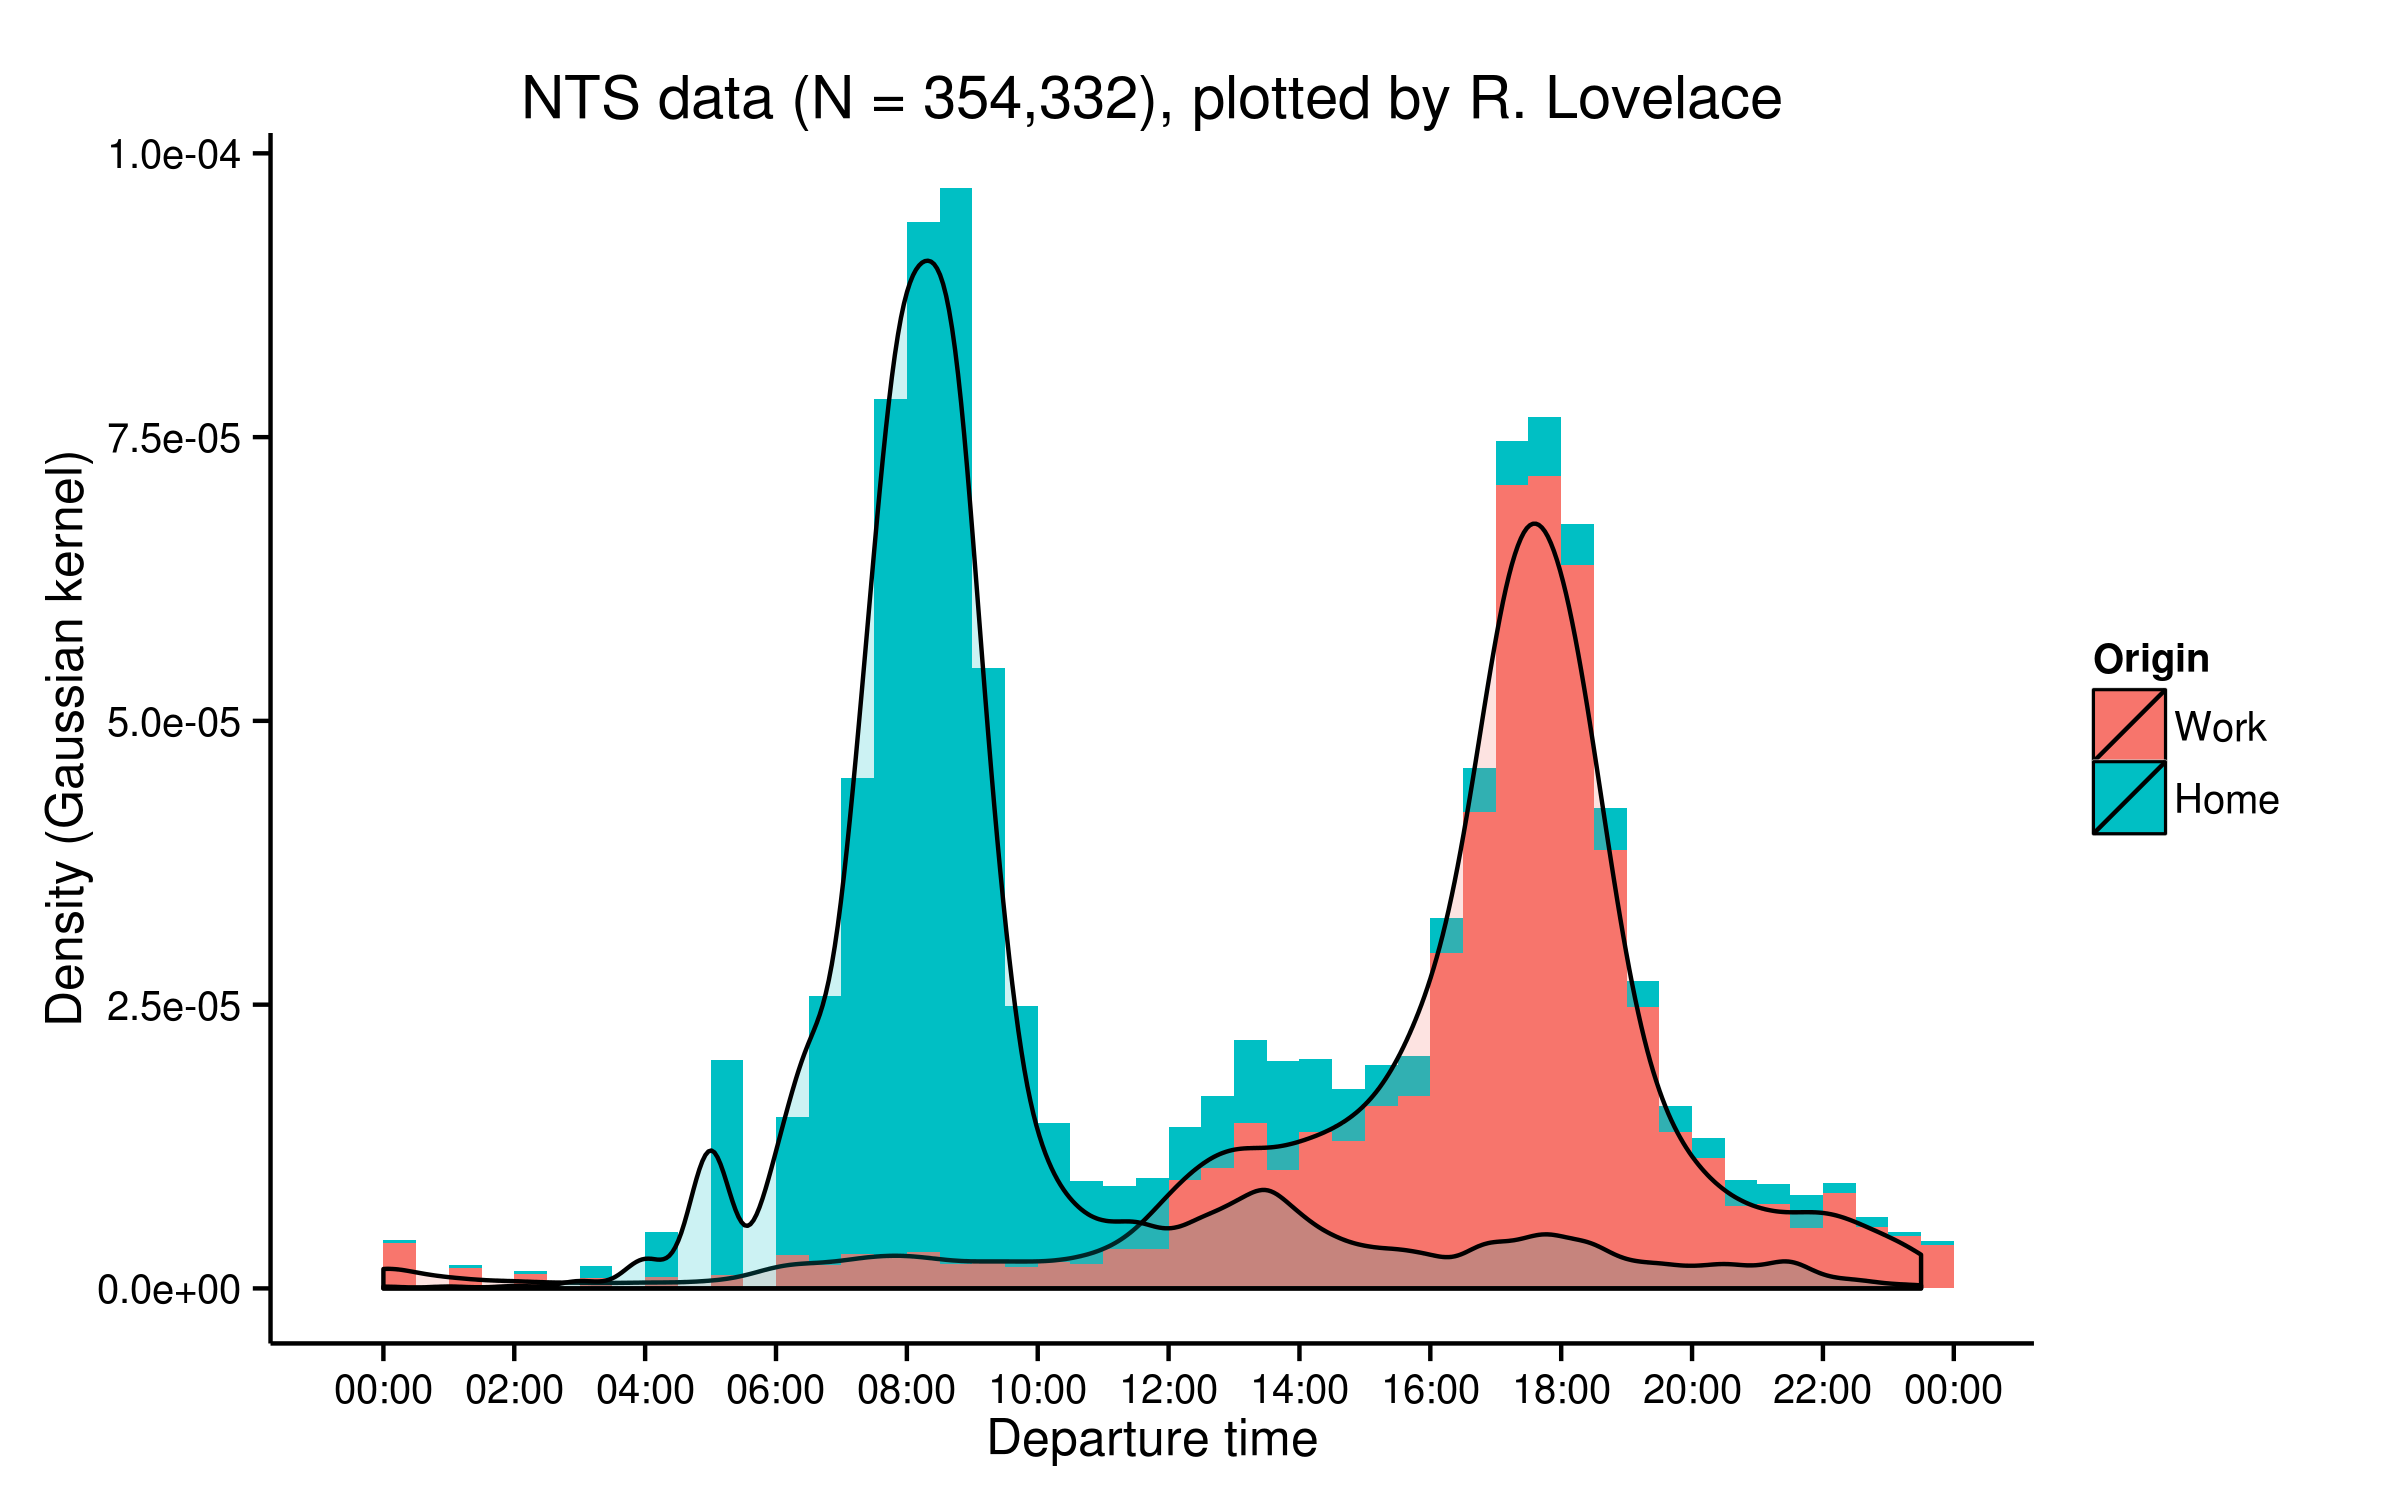
\includegraphics[width = 13 cm]{rush-hour}}
  \caption[The commuting `rush hours']
  {The concentration of commuter trips into morning
  and afternoon `rush hours'. Data source: the National Travel Survey.}
  \label{frushhour}
\end{figure}

\subsection{Behaviour}
The perceived impact of behaviour on vehicle energy use is demonstrated
by Energy Saving Trust's endorsement of `smart driving' to reduce fuel use
 and the AA's `eco-driving' recommendations to ``Save more than 10\% on
 fuel''.\footnote{See
 \href{http://www.energysavingtrust.org.uk/Travel/Driving}{energysavingtrust.org.uk}
and \href{http://www.theaa.com/motoring_advice/fuels-and-environment/drive-smart.html}
{theaa.com/motoring\_advice}
for further details on this advice.
}
A review of the literature to date supports the AA's claim:
\citet{Barkenbus2010} found that the handful of studies conducted
on the matter supported the view that promotion of environmentally conscious
driving could reduce fuel use by 10\%, although values ranged from 5 to 25\%
and more research is clearly needed on the topic.

This understanding could be harnessed in scenarios of the future, yet is of limited
use in determining the impact of variability in driving habits on \emph{current}
energy use. It is feasible, for example, that young males are less efficient drivers
due to faster speeds \citep{fleiter2007choosing} and harder acceleration
of this socio-demographic group. But this hardly translates into a
solid foundation from which to allocate certain socio-economic groups
to different efficiency bands, although this would be possible with the
spatial microdata. That is not to take away from the importance of driver
behaviour on energy use: 
empirical data from five passenger cars equipped with
logging equipment in Sweden \citep{Ericsson2001a} suggests that
fuel use per kilometre can vary widely depending on the driving style:
the standard deviation of average efficiency measurements was 50\%
of their mean value ($\sim$10 L/km). If sufficient evidence were available
it would, in theory, be possible to weight our efficiency estimates
by a range of variables known to be correlated with efficient and
inefficient driving styles. However, sufficient information does
not appear to exist anywhere, let alone for the UK at present.
Even if such a study \emph{did} exist at the national level,
there would be no guarantee that the relationships found would apply in the
same way to all areas.

Based on the evidence presented above, behaviour seems to be an important factor
to consider when estimating the energy costs of personal transport.
The complexity of the issue and lack of real world behaviour-energy use
measurement mean that it cannot be quantified and included in our model.
Behaviour is one more variable that adds uncertainty to our estimates,
and further research will probably be needed to reduce this uncertainty.

\subsection{Environmental conditions} \index{topography}
The impacts of environmental conditions on transport energy use is
a large and complex area about which relatively little empirical work has been
done (compared with the amount of work on the potential energy impacts of
projected technological change such as electric cars, for example).
The aim of this section is not to provide a comprehensive analysis of the
subject --- which could probably constitute a PhD
topic in its own right. The approach from the outset has been to acknowledge that
it is unrealistic to accurately quantify environmental impacts but flag what seem
to be the most important and easily modelled issues for discussion and
possible future research. `The environment' in itself is a vast domain,
ranging from the chemical composition of micro-climates to the soil
permeability. Many of these would have an impact on the energy use of
personal travel.\footnote{It is
likely, for example, that vehicle operating in areas with high levels
of particulate pollution would have increased energy use because
of clogged air filters, although the impact is likely to be negligible
compared with other factors. Similarly, one could argue that soil permeability
affects energy use indirectly through altered chances of flooding.
Again, the impact of this environmental factor is so slight and so hard
to measure that any accuracy benefits would likely small in comparison with
the costs of added complexity and the addition of untested assumptions.
}
For brevity, the focus is on environmental variables
which have been found to have an impact on transport energy use and
can realistically be studied using existing techniques. These are described 
in rough descending order of urgency of inclusion (a combination of ease
of accurate quantification and impact on energy use).


Topology has a large influence on energy use because extra
 energy is required to push vehicles and their occupants up hills. Without
 regenerative braking systems (which can never recover all the energy in
 any case), there is no way to restore this potential energy back into forms
 useful in the human economy, unless
 one is able and willing to roll down the hill every morning into work.
 Topology varies very little over time (unlike other environmental variables),
 has a large impact on energy use and there are high quality and ever-improving
 (due to the diffusion of low-cost remote sensing technologies such as LiDAR)
 datasets on its spatial variability. Despite this, there appears to be
 (based on searches of the academic literature) very little research on the
 impact of topology on transport energy use.

 \citet{Park2011} suggest that topology is the most important determinant of
 fuel use on the road network. In an earlier study, \citet{park2006energy}
 found that just a 1\% road incline could lead to an 18 \% increase in
 car energy use compared with flat roads and that a 6\% gradient,
 not uncommon in some UK cities, could lead to a 94\% increase in fuel
 consumption. This study was model-based. It would require
 real-world validation before the results were used to modify energy use calculations.
 It appears that many researchers do have a high level of confidence in their
 estimates of the energy impacts of topology, however. This is illustrated in
  studies investigating the potential for including
 topology in route-planning algorithms to maximise fuel economy
 \citep{minett2011eco, ahn2011eco}. This area therefore has great potential
 both to improve descriptions of current energy use and for creating
 scenarios of change. The Newtonian physics that describe the influence of
 topology on energy use should also make this issue fairly straightforward to
 include in high resolution geographical models of energy use.

Weather also has a major impact on fuel use, most notoriously through the
phenomenon of `cold starts', whereby cold temperatures affect the performance
of internal combustion engines due to a range of factors including cold
(and hence viscous) lubricants and fuels and catalysts.
In this matter, \citet[2422]{Weilenmann2009cold} found that
``fuel consumption increases almost linearly as a function
of decreasing temperature'' in the range of -20 to 20 degrees Centigrade,
with fuel use doubled at the low end of the scale. This effect is only
momentary however, lasting for $\sim$200 seconds according to one
paper \citep{Singer1999coldstartemissions200}. Therefore, the overall impact
of cold starts is likely to be negligible.

Temperature and other weather variables such as precipitation, sunshine
and wind also affect energy costs indirectly, via impacts on behaviour.
There is strong evidence of seasonal variability in car use linked to cold
weather, and \citet{Schipper1993} suggest that the seasonal impact could be
10\% or greater in northern countries. The modes of transport most exposed to
weather (walking and cycling) are also the lowest energy users, another reason
for expecting energy use to be higher in areas with, or during periods of
particularly inclement weather.

As with topography, there are readily available data about how key weather variables
vary over space, with the added complexity that these variables also change
continuously over time. The data collection, processing and matching to
discrete travel events would pose a major challenge to
researchers wanting to include weather as an input variable into energy use
calculations. However, provided strong empirical evidence of the
direct and indirect impacts of weather phenomenon (currently lacking) emerge,
these challenges are not intractable. This area of future research will
benefit from advances in computer hardware and software that will make it
easier to process and make sense of the `big data' contained within
the continuously variable time-space phenomenon that is weather.

Road roughness, including potholes, bumpiness and other irregularities
from the ideal of a perfectly smooth and flat motorway, like weather, have
both direct and indirect effects on energy use. The direct impact is primarily
on tire rolling resistance, about which there is strong evidence for
``substantial and measurable increases in energy losses'' due to
rough roads \citep{velinsky1980vehicle}. Increased energy use of up to
20\% are reported in this study. More recent work has been done on the topic,
but no conclusive impacts, that would be amenable to inclusion in a
large scale transport model, could be found from the literature.
This may be due partly to the complexity of the models employed to
estimate the energy costs of power dissipation through vibration
\citep{smith2011power}.

An indirect (yet somehow more tangible) impact of poor road quality on
transport energy use is that it can discourage people from buying
a low powered and energy efficient car.
This applies to the selection of sub-mode vehicle
type\footnote{For example,
a powerful 4 by 4 would be
preferred to a supermini in areas with very poor road conditions; a
mountain bike would tend to be used over a road bike if the path is
very rough.
}
as well as the more obvious inter-mode choice such as a
preference for driving over cycling
in areas where the cycle paths are relatively rough and potholed.
(On the other hand, extremely bad road conditions could encourage
walking and cycling if motor vehicles physically cannot pass, although
this is unlikely to be a common scenarios in developed Western economies
such as the UK). 


\section{Variability over time} % Variability by time
% could possibly split this into 3 subsections: fleet effs, mode shift + future
\label{s:eff-imps}
\subsection{The improving fleet efficiency of cars}
The previous section illustrates that fuel economy should not be seen simply as a
fixed number, such as 3 MJ/km for cars. Even at the aggregate level, the
average efficiency changes, depending on the year or 
geographical area of interest. Constant changes in technologies and
the range of models made available by car manufacturers, combined
with consumer trends such as the rush to ``4 by 4s'' in the early 2000s
drive these changes.\footnote{This has
been illustrated in a `gas guzzler' map by the author.
This time series choropleth map, uploaded to youtube
(see \url{http://www.youtube.com/watch?v=1r3joV82AuQ} ) ,
shows the proportion of
vehicle sales falling into the tax bands M and L in Yorkshire and the
Humber from 2002 to 2010. It is clear that this has had a major
(but as yet unquantified) energy impact.
}
Regulation is important too. In this context,
the European Union is instrumental: it is a legal
requirement that fuel economy and CO$_2$ emissions
are displayed alongside car adverts (presumably affecting buying patterns).
Perhaps more importantly, the European Commission has implemented
(struggling) legislation stating that the fleet-wide efficiency of
all cars must reach 130 gCO$_2$/vkm by 2015 \citep{Fontaras2010}, equating to
1.9 MJ/km.\footnote{Assuming an energy content of 14.6 MJ/kgCO$_2$,
which was calculated based on a 3:1 petrol:diesel split and
emission factors of 14.4 and 15 MJ/kgCO$_2$ respectively.
}
Because energy efficiencies are constantly shifting, it is important
to allocate times to our energy use estimates. The values presented in
\cref{sdirecte} were published in 2011, so are presumably valid for that
year. This is problematic when one considers that the constraint variables
taken primarily from the 2001 Census.
(Fleet energy efficiency dropped from 2.89 to 2.46 MJ/km between 1999 and 2009,
implying a 20\% improvement in fleet efficiency within that decade,
according to calculations from \citet[table 2.8]{Decc2011t}, a substantial issue).
It is not the purpose of this section, however, to apply modifiers to previously reported
energy efficiency estimates. This is because the values presented so far
come from a single source for all modes; altering the values for
one mode whilst leaving the others unchanged would not be consistent.
The purpose is to flag the issue and to
illustrate, in general terms, how fleet efficiencies have shifted and
how these changes can be accounted for.

Time-series statistics on energy use in transportation are
reported in \citet{Decc2011t}, which is based on a range of secondary data
sources over the past 40 years. Energy efficiency is reported in
the preferred European fuel economy units of l/100 km.
These values were translated into energy costs using a fixed conversion
factor of
33 MJ/l.\footnote{This
average energy content per litre of transport fuel was calculated
assuming a petrol:diesel split of 3:1 and volumetric energy densities
of 32 and 36 MJ/l for each fuel respectively \citep{Mj322010}.
}
The results show near constant improvements in new car energy performance
since at least the late 1970s, as illustrated in \cref{fig:etime}.
The average fleet-wide (including new and
old cars) efficiency can also be derived from \citet{Decc2011t}, based on
information on total vehicle kilometres travelled and energy used by cars.
% Describe the Decc dataset in a little detail, then the Schipper/Dft one, then
% a bit comparing both of them and comments on rates of change. Simple!
The pattern of fleet efficiencies relative to new car efficiencies
presented in \cref{fig:etime} is arguably predictable, as the former
appears to have more `inertia', trailing the latter
by a few years, and falling by an average of 1.7\% year over the last 10
years.\footnote{Between 1999 and 2009 the fleet
efficiency of British cars fell by 15\%, from 2.89 to 2.46 MJ/km. The largest
annual change was  between 2008 and 2009, in which time energy use
per unit distance dropped by 2.9\%.
}
Improvements in new cars have happened more quickly, averaging 2.5\% per year
over the same period. The inertia of the existing fleet has been reduced
somewhat by the UK's subsidised `scrappage scheme', although it still has
major impacts for projections of energy efficiency into the future. 
\begin{figure}[h]
  \centerline{
    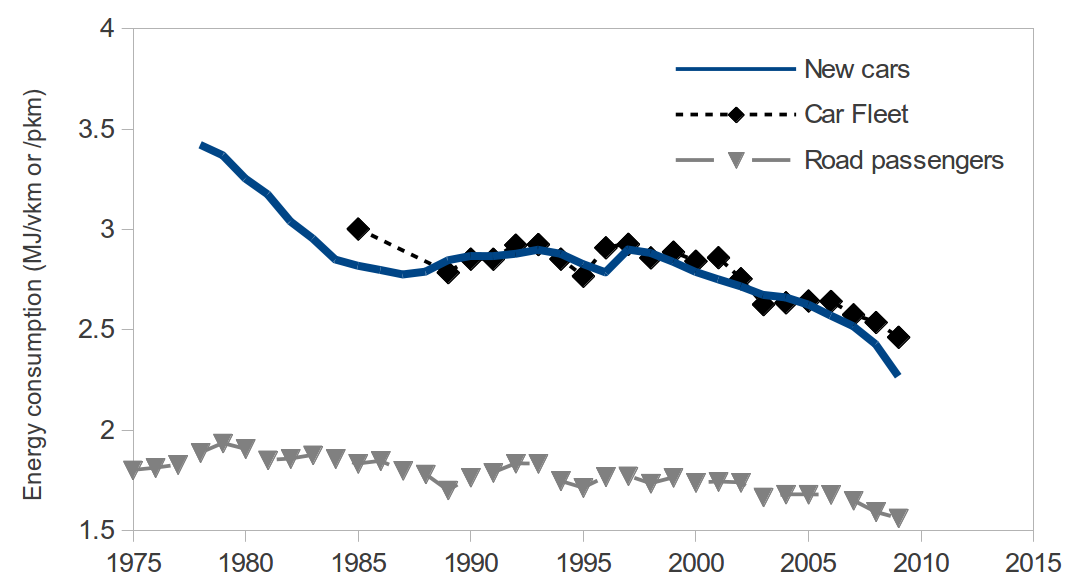
\includegraphics[width = 14 cm]{etime.png}}
    \rule{35em}{0.5pt}
  \caption[Fleet efficiency of UK vehicles over time]{Energy consumption of new
cars, the entire car fleet, and the energy intensity of road passengers
transport kilometre over time. Data: \citep{Decc2011t}.}
  \label{fig:etime}
\end{figure}

The above time-series data can be corroborated by a more recent statistical
release from the Department for Transport \citep[table VEH0256]{Df2013licencing}.
In this dataset, the number of car sales in each emission band (from
``up to 100'' to ``over 255 g/km'') is reported every quarter since Q1 2003
until Q1 2012, alongside estimates of the average emissions of new car sales
each year. Using the same conversion technique described in \cref{sdirecte},
this was converted into average efficiency values in SI units. The results
inspire confidence: the values are within 7\% of those derived from
the \citet{Decc2011t} data. The accelerating downward trend continues for new cars,
falling by an average of 2.7\% per year between 2002 and 2012 and by over
4\% per year since 2007, as illustrated in \cref{fnatefic}.
The dramatic acceleration in the rate of efficiency improvement
seems less impressive when placed in the broader perspective (and with a
y axis that starts at the origin):
\citet{Df2013licencing} and \citet{Decc2011t} figures are compared in
the same graph in \cref{fnatefficall}, which also shows historical data from the USA
and the UK \citep{Schipper1993}. It is interesting to note from this graph
that rapid improvements in energy efficiency can be achieved through regulation:
following the aggressive implementation of the
Corporate Average Fuel Economy (CAFE) standards in the wake of the 1970s oil
crises, the average fuel use of new cars dropped on average by more than 5\%
per year in the decade following 1973, before levelling out during the
1980s.


\begin{figure}[h]
  \centerline{
    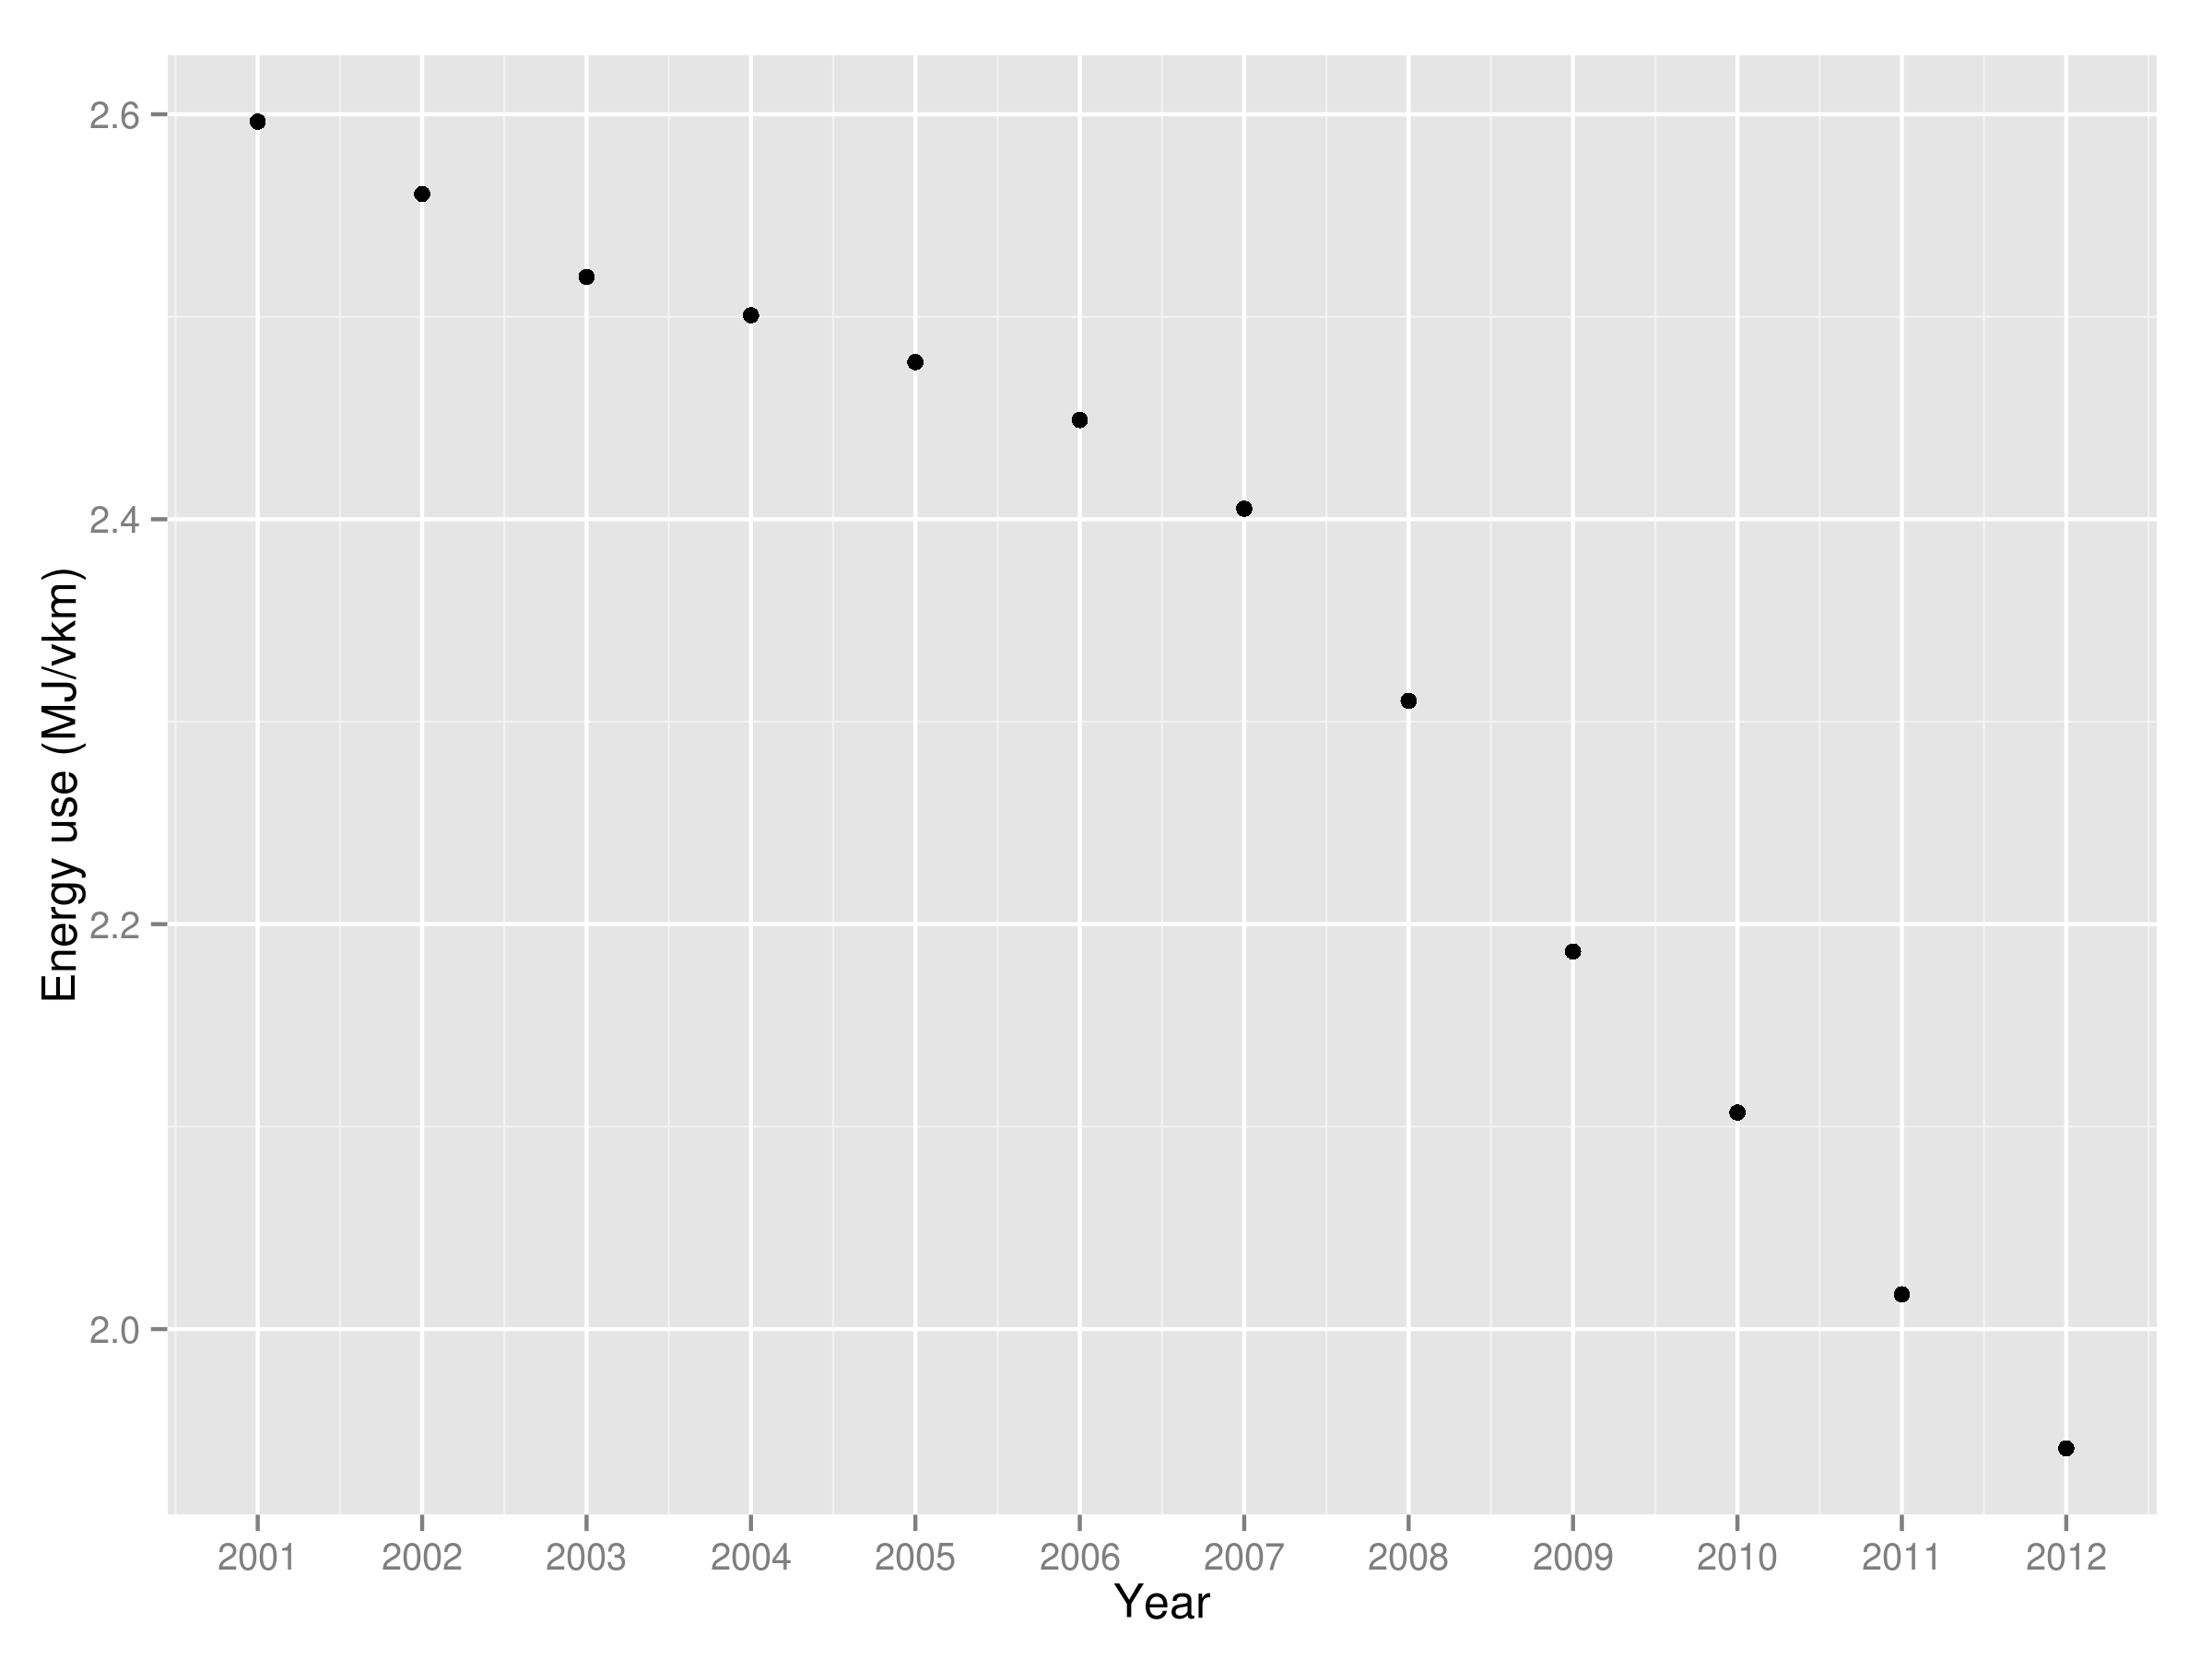
\includegraphics[width = 14 cm]{natefic}}
    \rule{35em}{0.5pt}
  \caption{Comparison of UK car fleet efficiency estimates over time \citep{Df2013licencing}.}
  \label{fnatefficall}
\end{figure}


\begin{figure}[h]
  \centerline{
    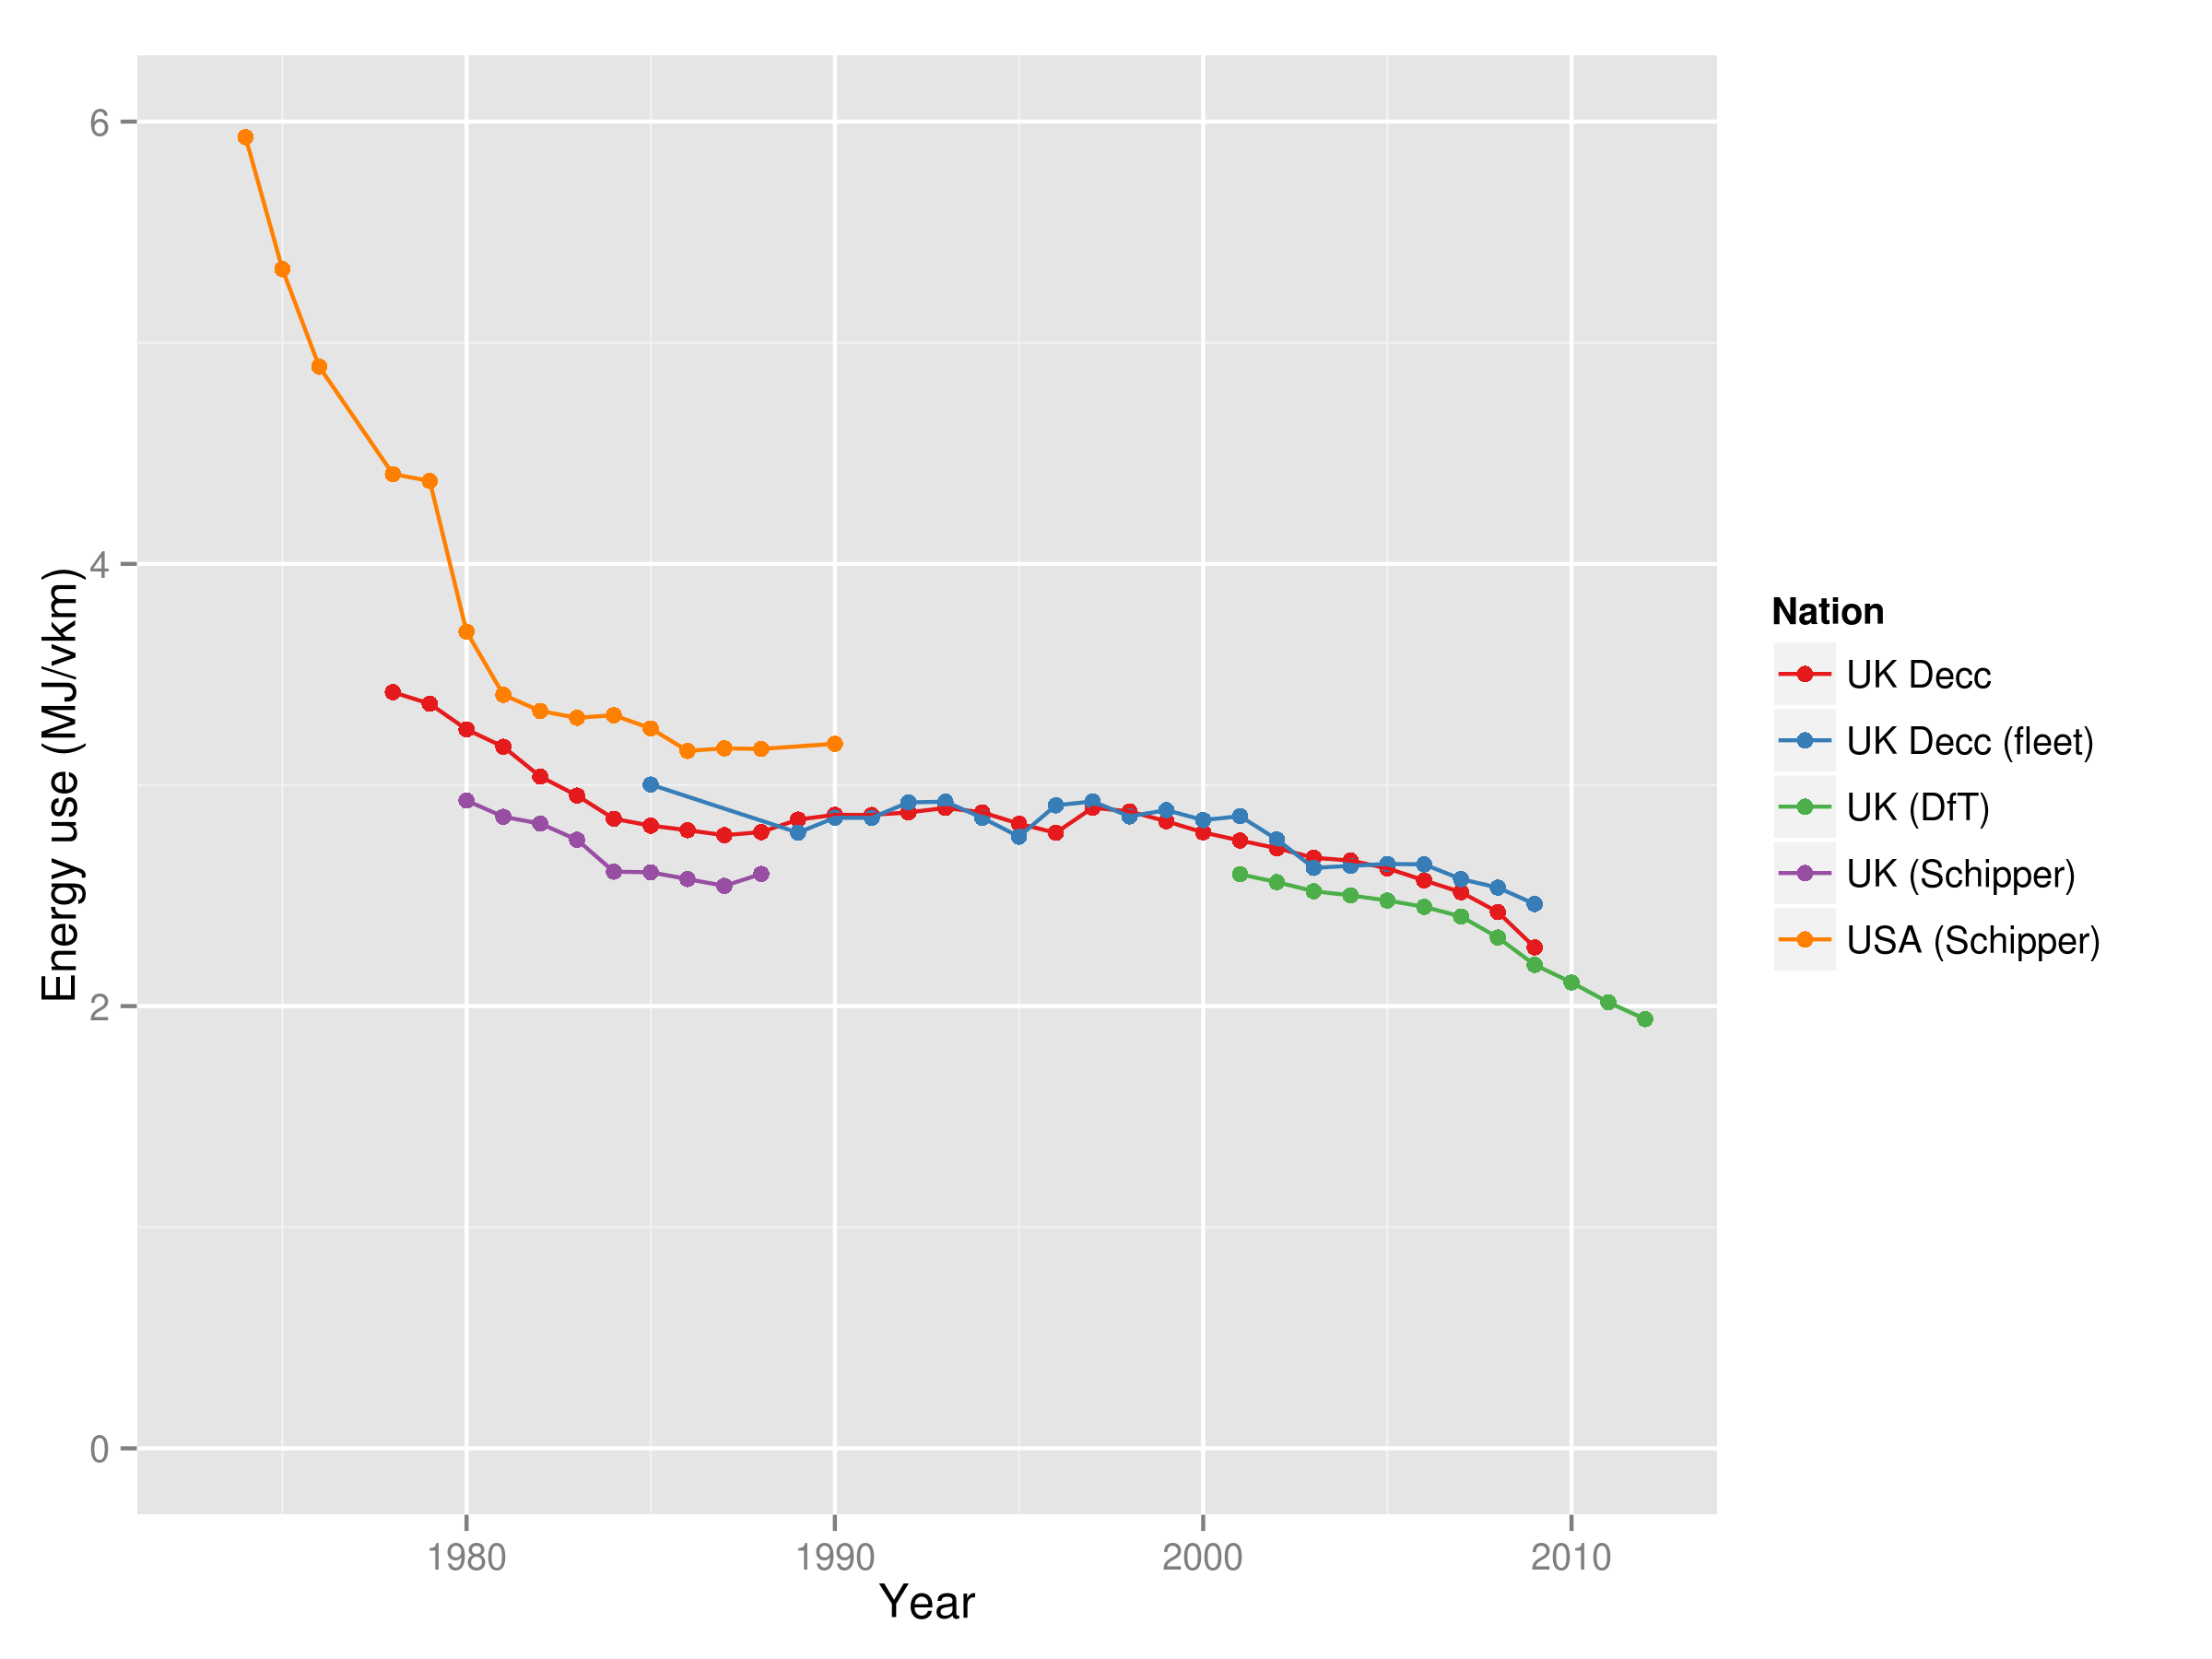
\includegraphics[width = 14 cm]{natefficall}}
    \rule{35em}{0.5pt}
  \caption[Fleet efficiencies of new cars in the UK and USA, 1977-2012]
  {Fleet efficiencies of new cars in the UK and USA, 1977-2012.
  Data calculated from 
  \citet{Schipper1993} (UK1, USA), assuming an energy content of fuel of
  32 MJ/l, and the Department for travel
  \citep[table VEH0256]{Df2013licencing}, assuming a conversion factor
  of 14.4 between kg of CO$_2$ and MJ.}
  \label{fnatefic}
\end{figure}

The imperfect match between the estimates of energy efficiency over
time from two independent official sources (both of which are
more than 10\% below the 3 MJ/km figure calculated from
\citet{Defra2011} in \cref{sdirecte}), combined with the difficulty of `measuring'
energy economy in
practice
\citep{Schipper1993},\footnote{CO$_2$
emissions tests, from which
DECC's $Ef$ estimates are derived, are conducted in laboratory conditions on
new cars. Therefore, the resulting data may not be 100\% applicable to reality.
Cold starts, driving behaviour, and congestion all influence $Ef$, meaning its
variability is probably much greater than that illustrated here
}
suggest that
the \citet{Decc2011t} estimate of $Ef$ should be treated as a ``best estimate''
rather than an exact value that is set in stone. As highlighted throughout
\cref{svariable}, the performance of vehicles varies greatly depending
on a range of factors, so it is unlikely that even rigorous tests that
try to emulate real world driving match perfectly from actual figures.
This point is emphasised by the ``real mpg'' project hosted by
www.honestjohn.co.uk, whereby drivers are encouraged to enter their
vehicles' fuel economy data and compare the results with official values.

% Over the last 3 decades, transport to work in the UK, and in many other
% developed economies, has been dominated by %!!! add later???
% cars. Walking, buses, and trains/metro are, in descending order, the next most
% popular forms at the national level. Within the region of Yorkshire and
% the Humber (YatH), the overall pattern is the same, although buses are used more
% than the national average. This may be due to relatively low usage of railways
% in the region. These similarities and differences are illustrated here by the
% 2001 Census (Table x), and are persistent over time (evidence).

% Table x: Proportion of trips made by different transport forms at national and
% regional levels, from the 2001 Census. Note the proportions exclude the ~8\% who
% work from home.
\subsection{Modal shift}
Because the differences of energy use between modes are greater than the
differences within modes (amongst current, commercially viable and desirable
models at least),
modal shift probably has the greatest potential to alter energy costs of commuting
over time. The spatial microsimulation approach to estimating energy costs used
here assumes that mode and distance categories are already known from the
census --- these constrain the spatial microsimulation model and thereby form
the basis of our energy calculations. This a-priori knowledge about the key attributes
of commuting behaviour allow us to focus on the more technical aspects influencing
the energy costs of travel to work. This is useful, and represents a step forward
in terms of method (there would be little point in attempting to quantify
impact of many variables if not even the commonest modes and distance bands
were known). However, it also brings the risk that mode and distance, which ultimately
determine the energy costs of work travel, are taken for granted.
It is this issue to which our attention now turns. The focus is on past modal
shifts  to provide understanding about the scale of the
shift in our travel to work patterns that have happened over the past 100 years.
(Speculation about and scenario building for future shifts are tackled
in a later chapter.)

Increasing car dominance is the most striking feature of 20th Century transport
to work. Data from a large (n=1010) survey extending back to the 1890s
illustrates this shift (\citealp{Turnbull2000}; \cref{fturnmode}).
The sampling technique used in
this longitudinal survey (self selection) and lack of national data for
corroboration before 1971 mean that these historical data may not precisely
match the national picture. However, the close match between the results and
recent surveys suggest that these issues ``have not unduly distorted the picture
of commuting'' \citep[p.~13]{Turnbull2000}⁠.  The data also show that commuter patterns can
shift quickly in times of rapid economic and technological change: between 1940
and 1960, for example, the proportion of respondents  driving to work increased
from 6 to 36\%, a 6-fold increase in 20 years! When this modal shift data is
converted into energy use estimates, based on the (unfounded but useful)
assumption of fixed distances and efficiency of each mode taken from recent
data, the results are striking (\cref{flongip}): it appears that current
commuter energy costs are around an order of magnitude greater than they were
at the beginning of the century, with almost all the growth attributable to
the rise to dominance of the car.

\begin{figure}
 \centerline{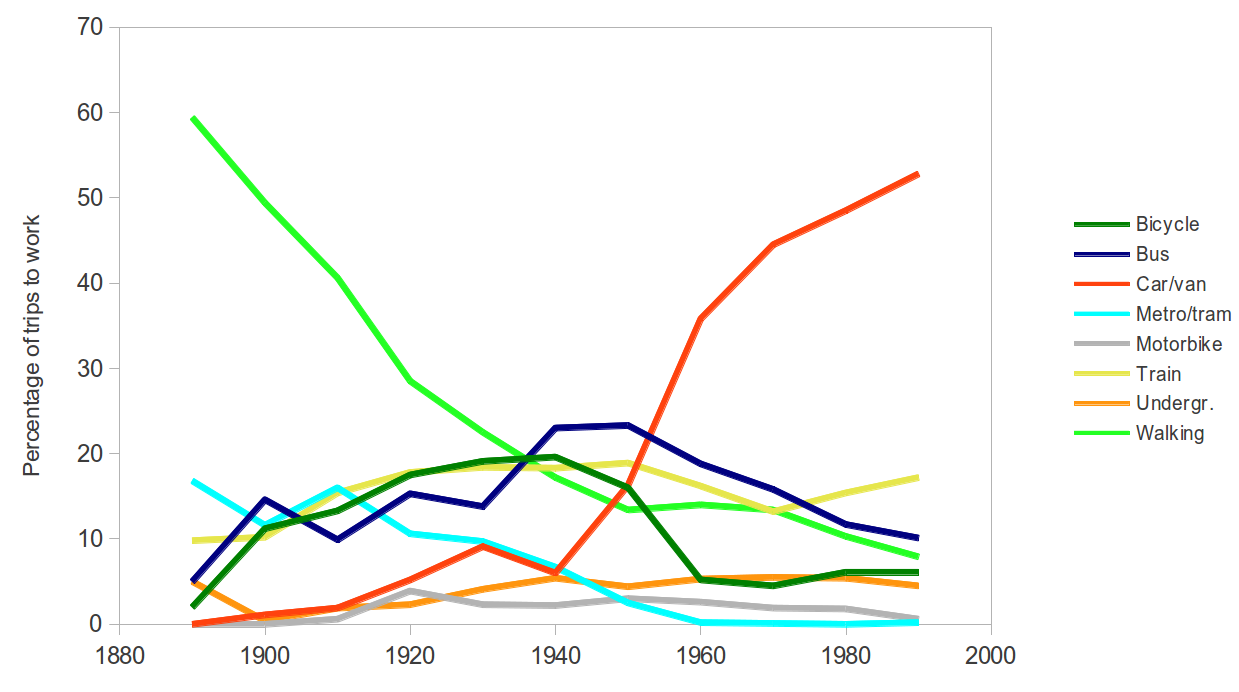
\includegraphics[width=15 cm]{longi}}
 \caption[Mode of transport to work, 1890-1990]{Mode of
 transport to work, 1890-1990, from a self-selected sample of
1010 respondents (data from Turnbull, 2000).} \label{fturnmode}
\end{figure}

\begin{figure}
 \centerline{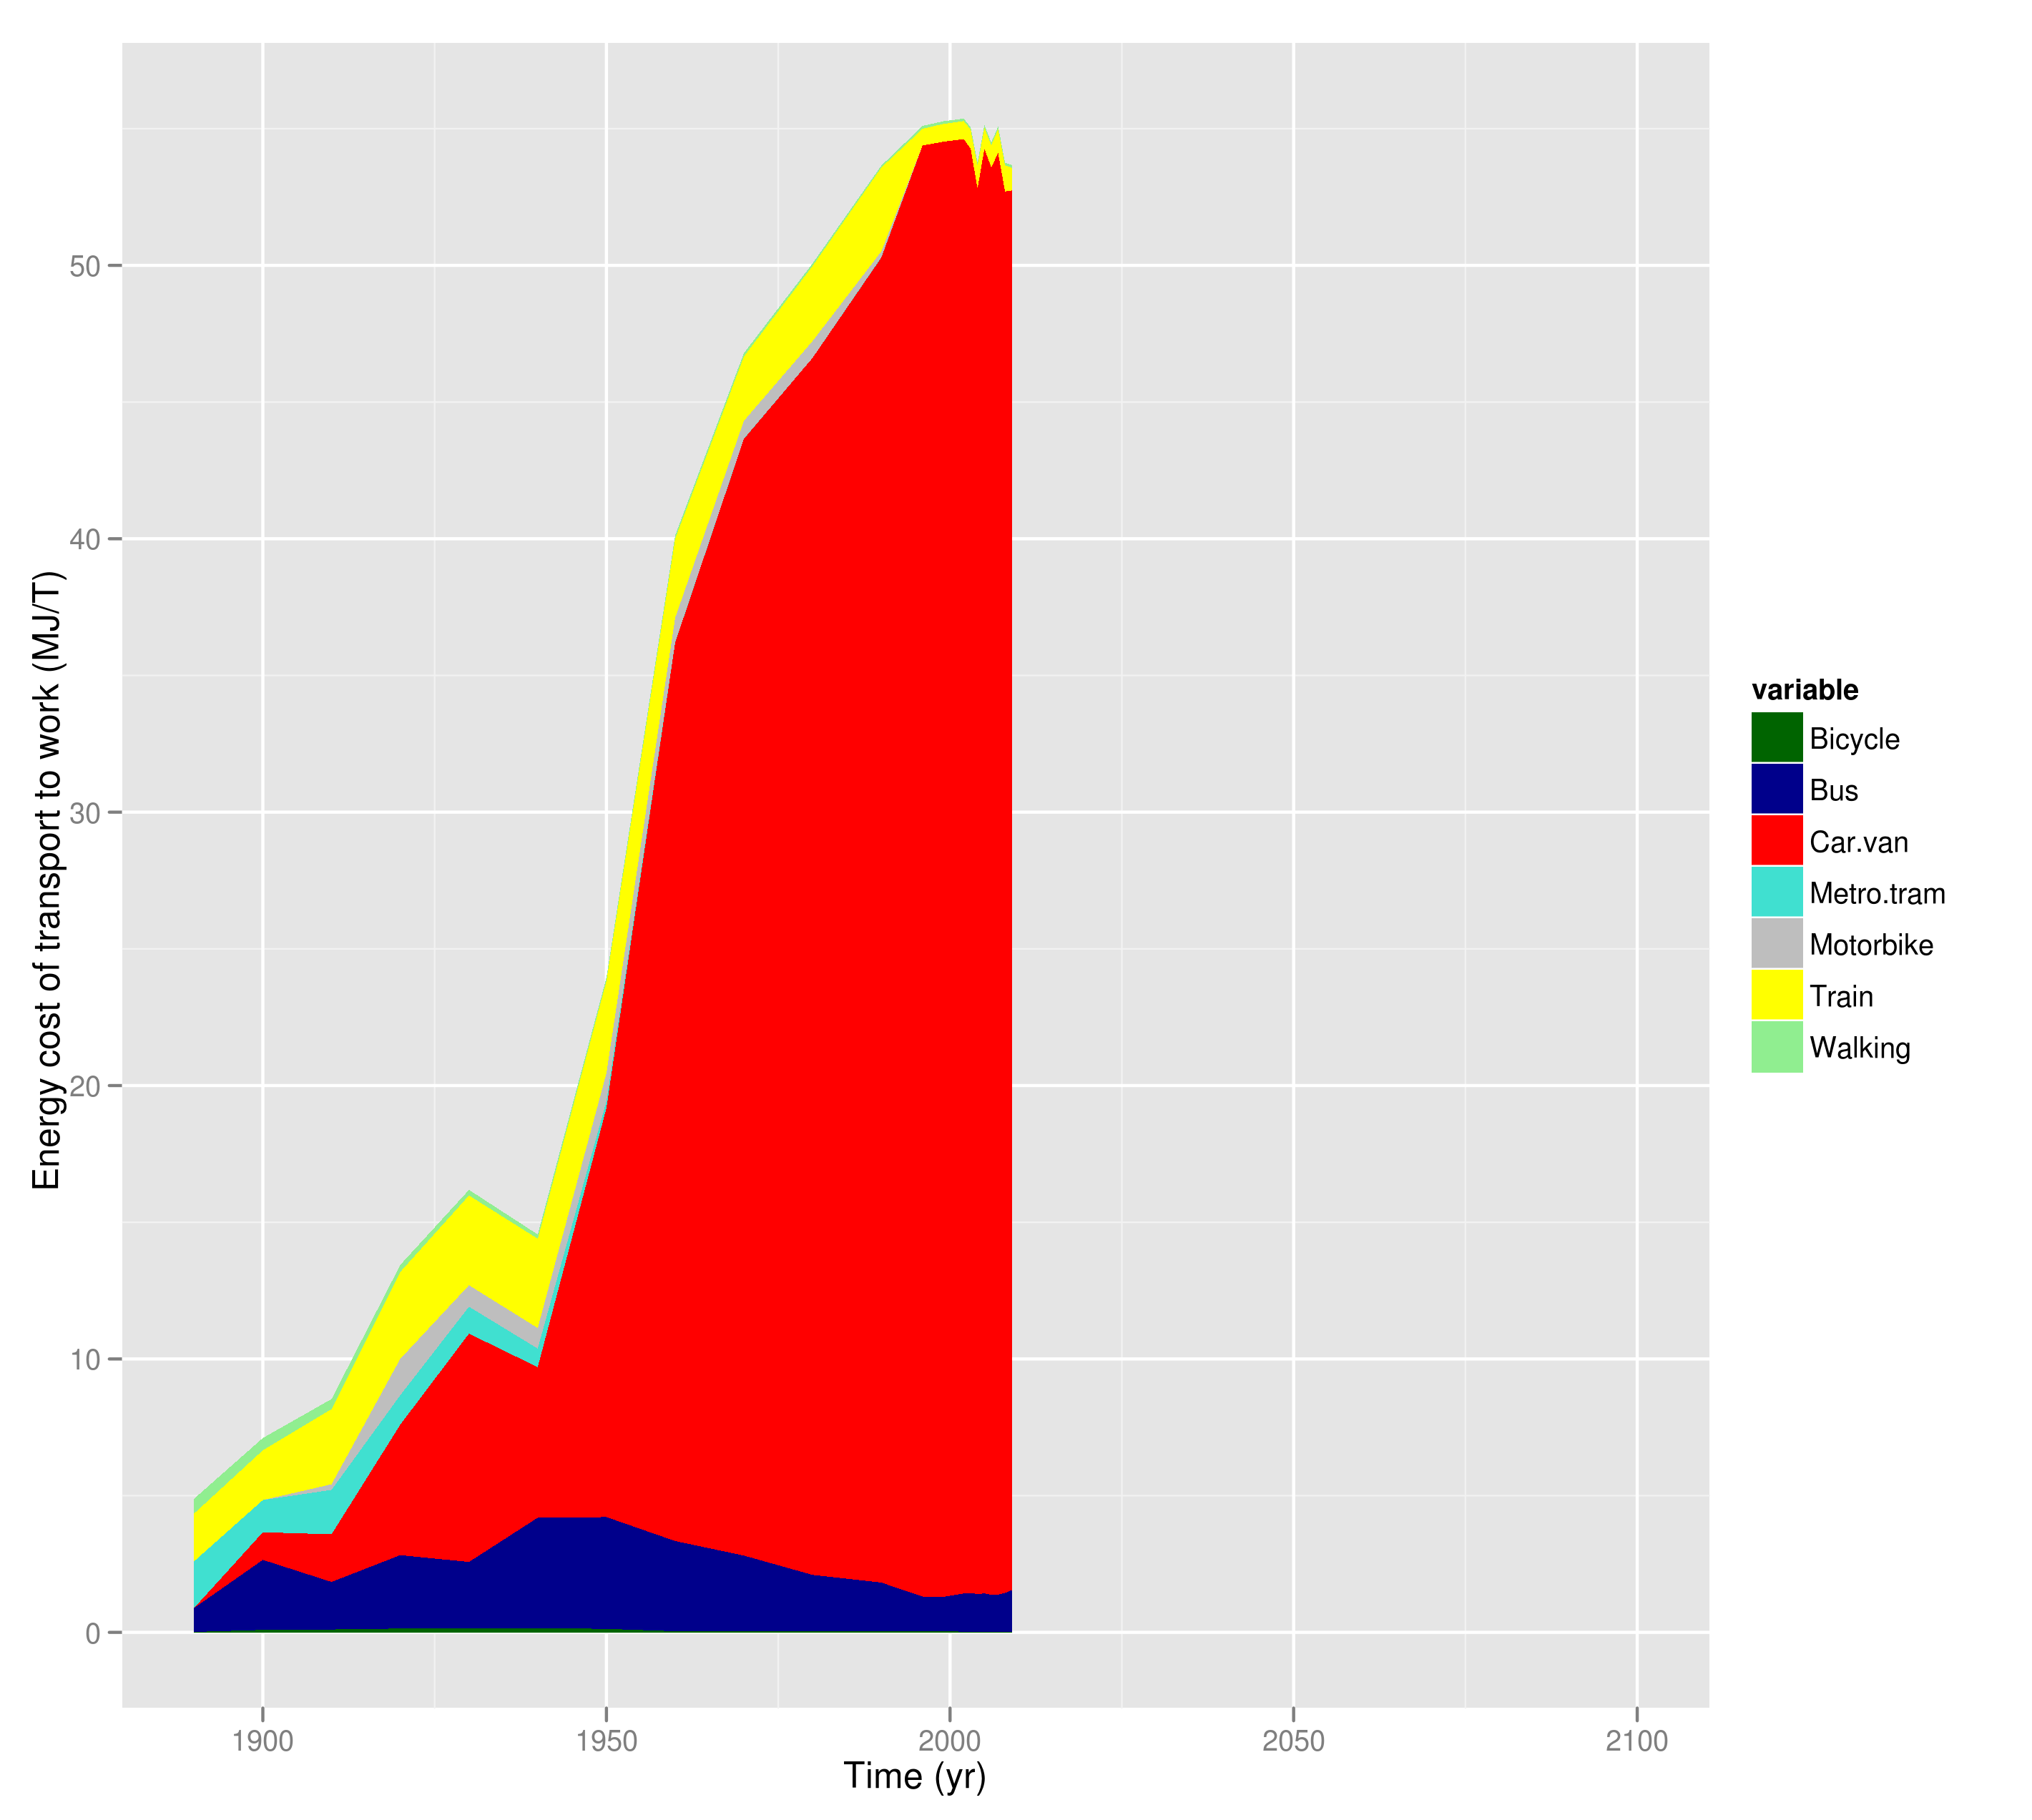
\includegraphics[width=15 cm]{longip}}
 \caption[Estimates of energy use per commuter trip, 1890-1990]
 {Estimates of energy use per commuter trip, 1890-1990.}
\label{flongip}
\end{figure}

Recently, rates of modal shift at the national level
have been much slower, however, as illustrated by \cref{fbhps}.
\begin{figure}[htbp]
    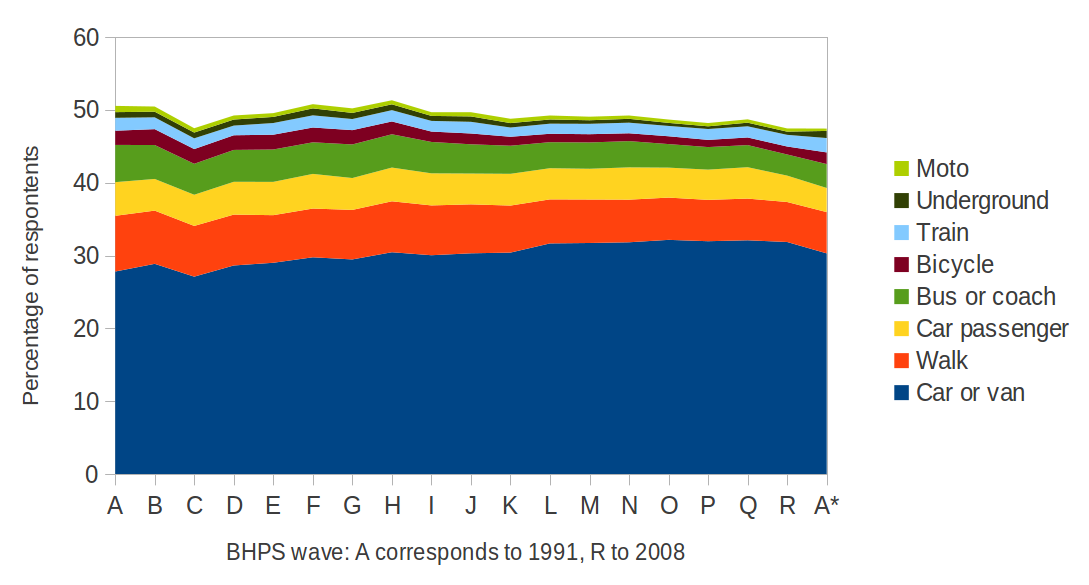
\includegraphics[width=12cm]{BHPS-long}
  \caption[Modal split of travel to work over two decades]
  {Modal split of travel to work over time, from the BHPS and
  (for wave A*) the USd.} %%% could update with methods
  \label{fbhps}
\end{figure} %!!! re-add?
% The shifting geography of commuting in Yorkshire and the Humber
Knowledge of the spatial distribution of transport patterns, and how they have
changed, is prerequisite to understanding geographical variation in the energy
costs of work travel. Rather than merely taking a snapshot of current patterns
overall, time-series maps can illustrate how the geography of
different modes has shifted over time, in addition to the non-geographical
aggregate shifts.
Cars have clearly risen to dominate the
UK's work travel (\cref{fturnmode}), but this has not happened uniformly over
space. This is dramatically illustrated by plotting the number of areas in which
driving a car (as opposed to being a car passenger) is a more common form of
commuting than all other commuter modes put together (\cref{f1981}).

\begin{figure}[htbp]
  \centerline{
    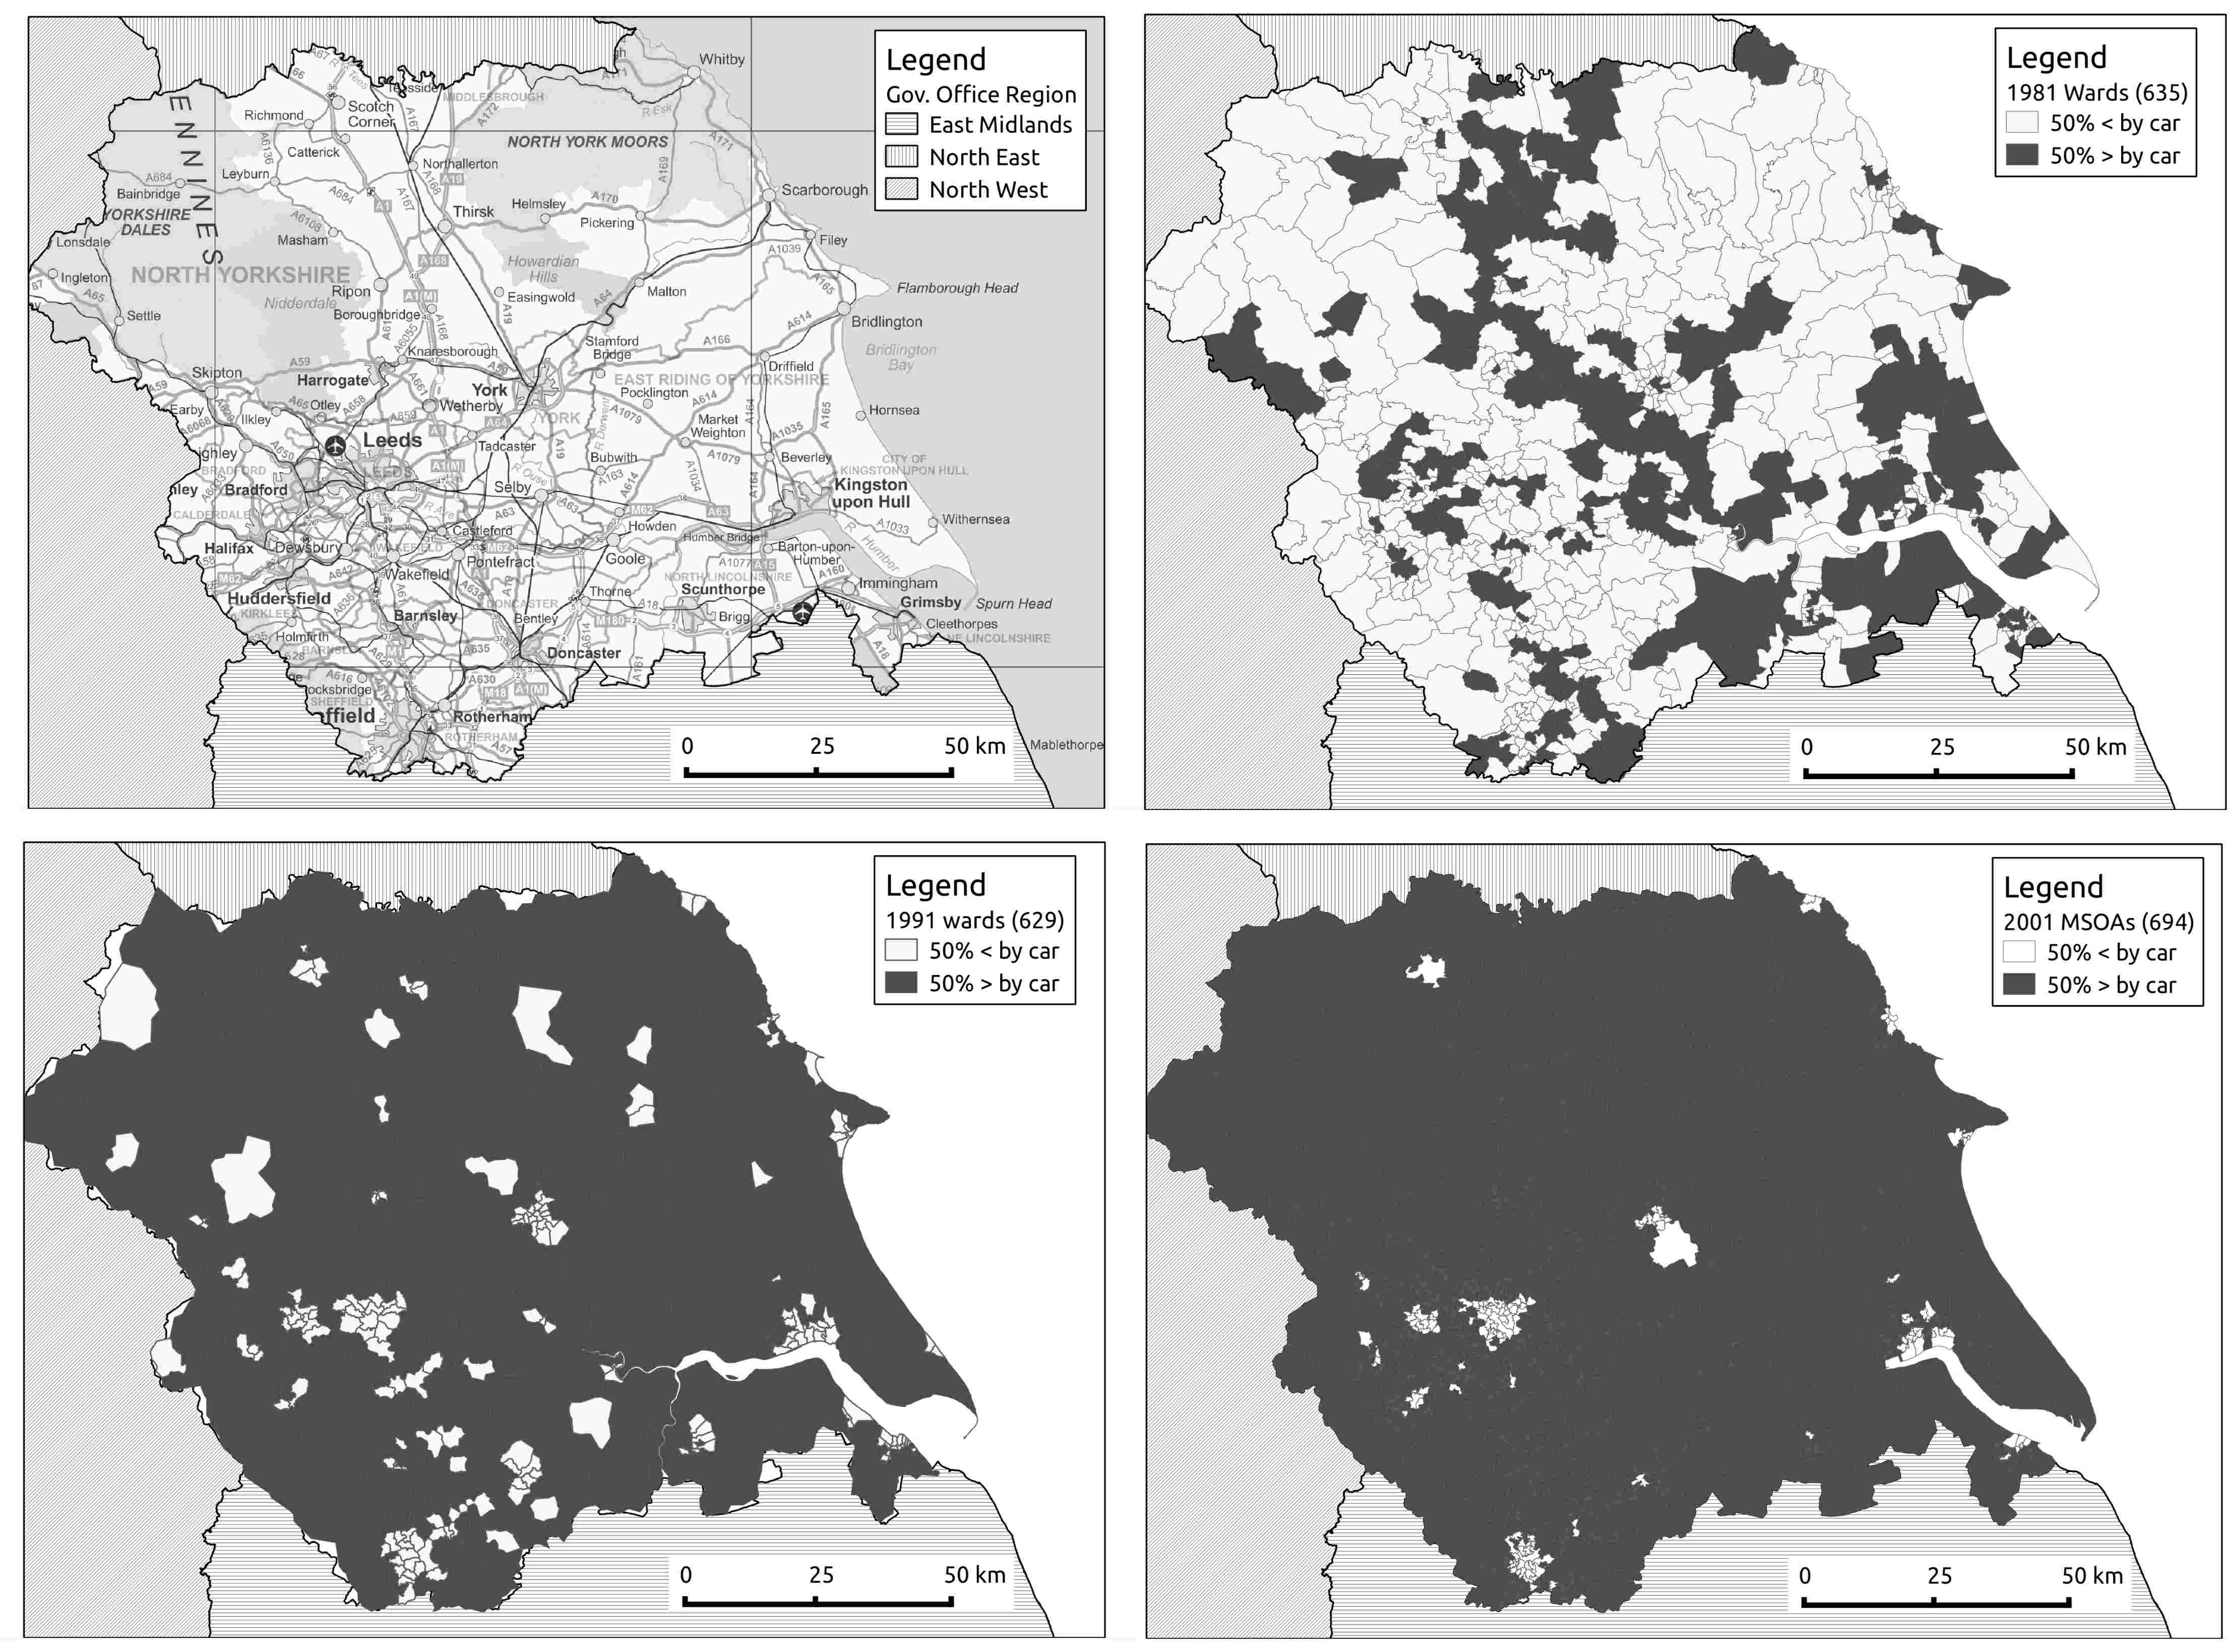
\includegraphics[width=16cm]{1981-2001}}
  \caption[The growing dominance of the car, 1981 to 2001]
  {Areas in which driving to work accounts for more than half of all
  commuter trips in Yorkshire and the Humber. Ward level data from
  Casweb.} %%% could update with methods
  \label{f1981}
\end{figure}

The maps show that, although car drivers were already by far the most common
type of commuter by 1980, they still only constituted more than 50\% of the
total, excluding those who work from home, in just over ~1/3 of administrative
areas (241 of 635 wards). Also of interest is the fact that many of these areas
were urban, such as Ecclesall in central-west Sheffield, and city centre wards
in Harrogate, Leeds and York. By 2001 car dominance was greater. Car drivers
outnumbered all other commuters combined in 81\% of MSOAs (563 of 694 areas).
However, the trend for relatively high urban car use had reversed by this stage.
This is clear from the patches of white which are almost exclusively limited to
densely populated urban centres in 2001 \cref{f1981}.
% This shift in car dominance from an urban to a rural phenomenon can be
% illustrated by plotting the proportion of trips made by car against population
% density (Fig. X still to do...).


\subsection{Future efficiency improvements}
A range of technological options exist to make cars `fit for their purpose'
in the short term \citep{plowden2008cars} and remove their dependence on
fossil fuels in the long term by electrification. However, when talking
about technological change in transport, there is a tendency to
idealise and exaggerate the rate of change possible.\footnote{A
good example of this tendency is illustrated by an article published
by the British Broadcasting Corporation (BBC) seriously
touting the possibility of flying cars catering for personal travel needs in
the future: ``As motorways become more and more clogged up with traffic,
a new generation of flying cars will be needed to ferry people along skyways''
\citep{BBCNews}.
If even the well-respected BBC could place sensation before evidence,
there is no reason to suggest that media or funding-hungry academics
could not do the same.}
In reality, the energy requirements of moving a large metal (or perhaps
plastic, carbon fibre or other material yet to be commercialised)
box around at high speed are constrained by Newtonian
physics, and are always going to be high compared with walking, cycling or
the best public transport modes \citep{MacKay2009}.
Focussing on the technologies that have been proposed and are receiving
serious funding for development, it is clear that there are no `golden
bullets' to dramatically improve the efficiency of cars
(the same would apply to other modes). This is illustrated in \cref{faltves}.

\begin{figure}
 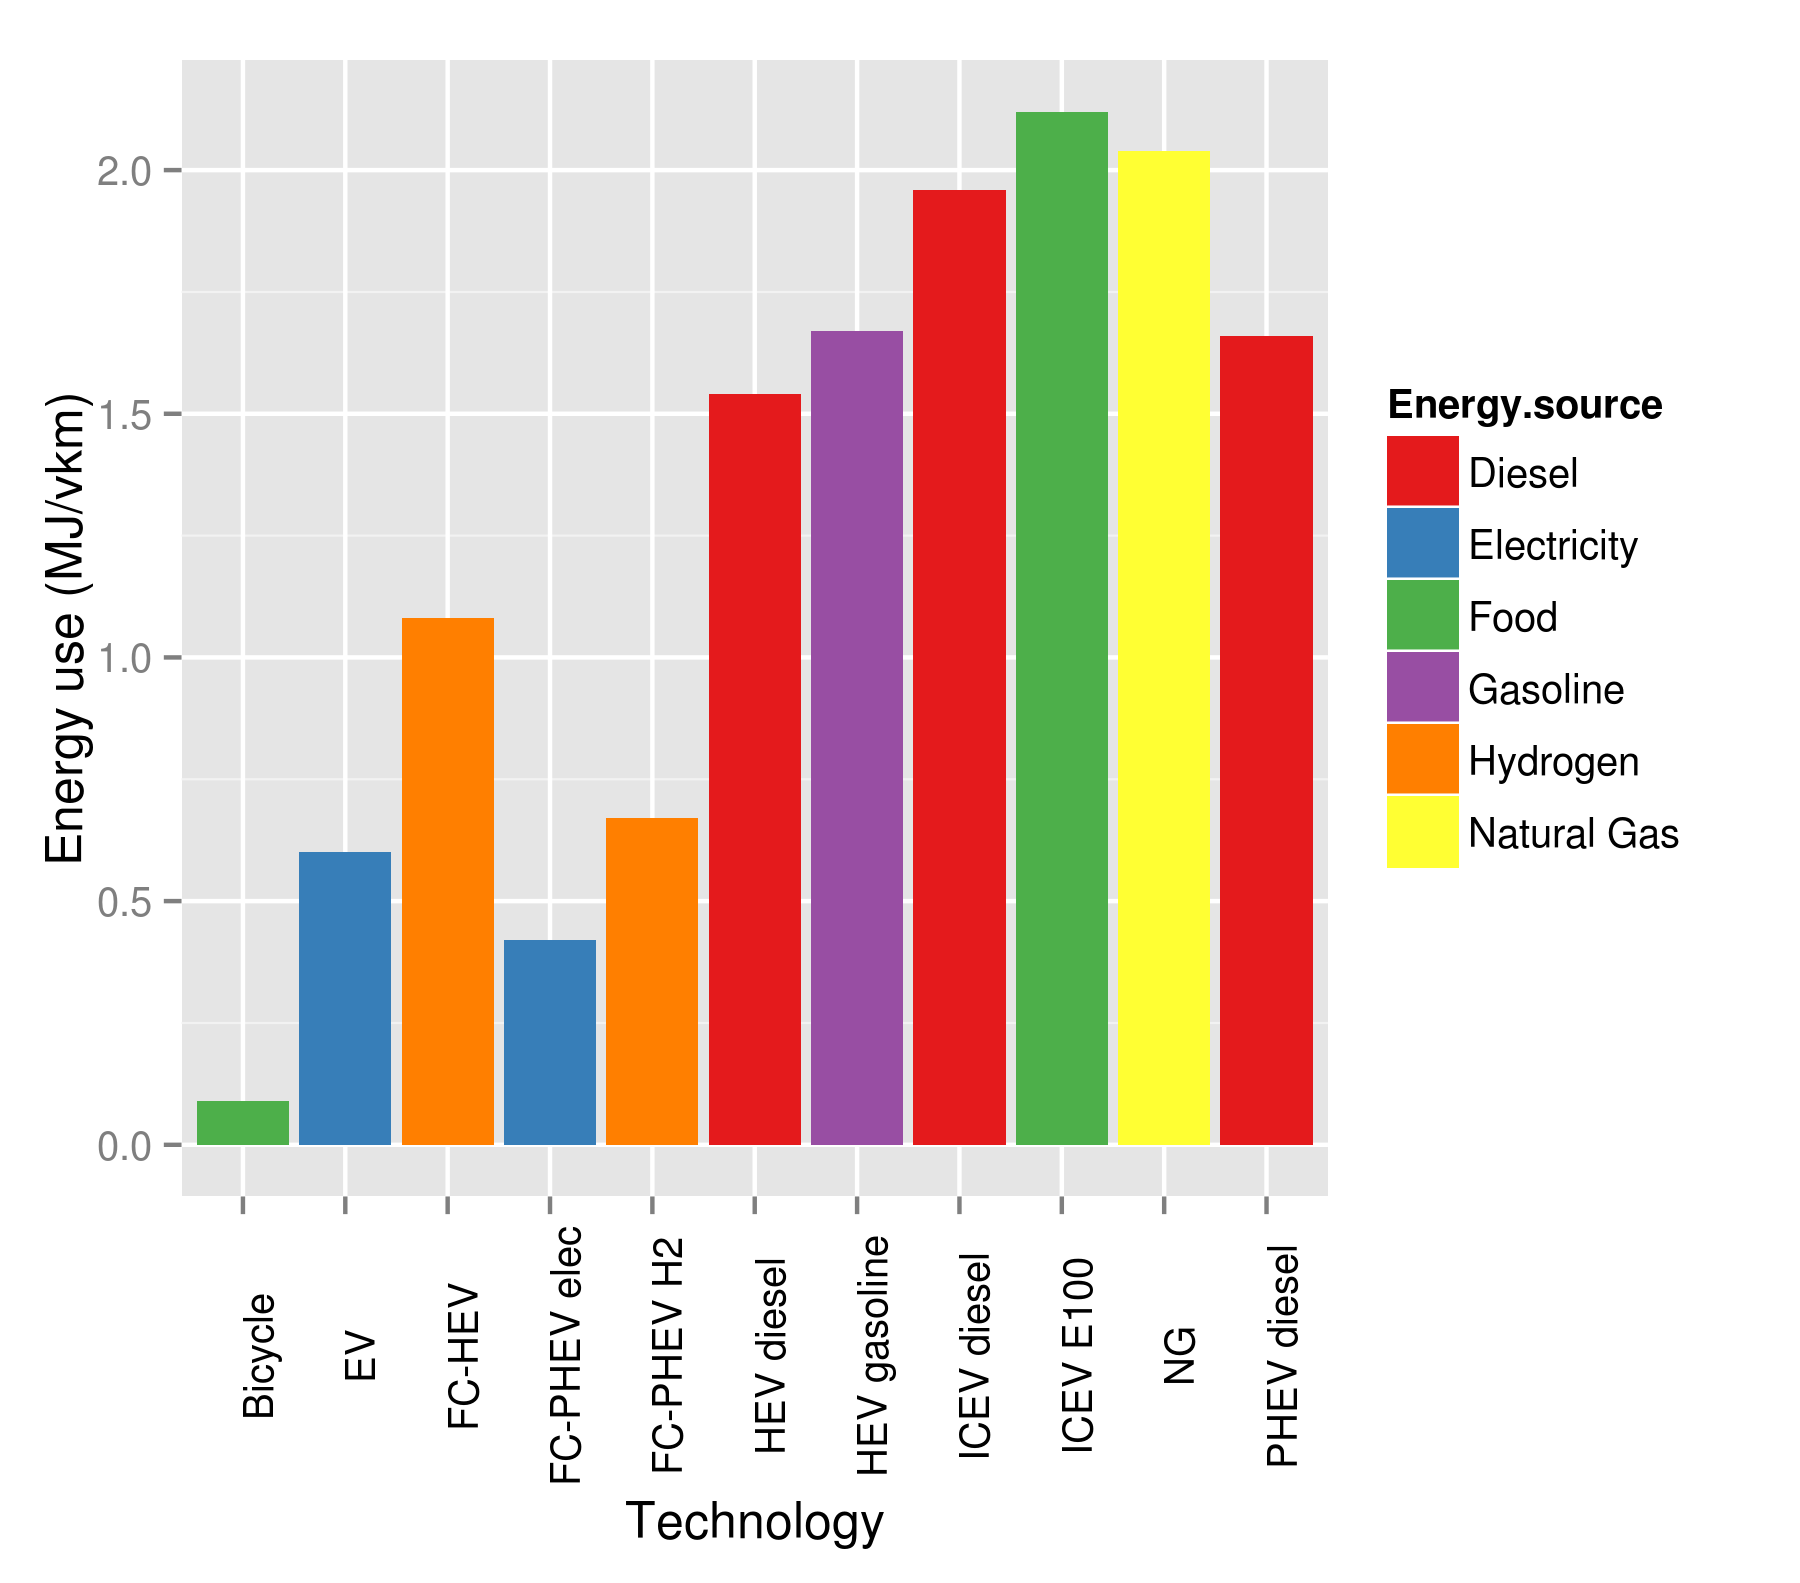
\includegraphics[width=14cm]{altves}
 \caption[Fuel energy use of future car technologies]
 {The fuel (or `tank to wheel', TTW) energy use of a selection of
 the most promising future car technologies as they currently stand, from
 \citet{Baptista2012} alongside our own figure for the bicycle, for comparison.
 The acronyms are
 as follows: EV (electric vehicle), FC-HEV (fuel-cell hybrid electric vehicle),
 PHEV (plug-in hybrid electric vehicle), ICE (internal combustion engine) and
 NG (natural gas).} \label{faltves}
\end{figure}

Some of the new technologies presented in \cref{faltves} seem quite promising,
with a few currently offering 3 fold energy savings compared with conventional
cars. However, in all four cases which require below 1.5 MJ per kilometre, a
glance at the energy source reveals the problem: each relies on either
electricity --- which requires around double
the energy content in fossil fuels to produce as is stored in the car's
battery (\cref{ssystemlevel})
--- or hydrogen, which is a very long way from being (and may never be)
commercially viable.\footnote{Hydrogen
is very wasteful of energy to produce \citep{Smil2008}. It
is difficult and energy intensive to store --- due to high pressure and low temperature
requirements --- so is rejected as a realistic option to transition away from
fossil fuels by some scientists \citep{MacKay2009, kreith2004fallacies}.
This judgement is followed here, avoiding the potential distraction of the
`hydrogen economy' advocated by some researchers (e.g.~\citealp{Kleijn2010}).
}
Still, pending the rapid roll-out of new renewable and nuclear generating
capacity \citep{dyke2010impact},
battery electric vehicles (BEVs) clearly have huge
potential to reduce energy costs due to the very high efficiencies of
electric motors ($>$90\%), if their worst problems can be overcome.
These include:
\begin{itemize}
 \item Reliance on rare earth metals for the motors and electronics.
 \item Additional strain on an ailing electricity grid \citep{dyke2010impact,
 webster1999can}.
 \item The fact that electric cars are
more expensive than comparable conventional cars due primarily to the costs of
high quality lithium-ion batteries.
\item Poor range and (discounting a few models) performance.
\end{itemize}
Each of these factors have contributed to
the poor UK sales of electric vehicles observed in 2011
\citep{AdamVaughan2011} and 2012 \citep{DavidCornis, Massey2013elecmail}.
In combination, these factors are likely to limit the penetration rate of BEVs below
more optimistic projections (e.g.~\citealp{Shepherd2012}).\footnote{Sales
in the USA and Germany, two of the world's largest and most lucrative car
markets, have also been poor \citep{Hepker, Mihalascu}.}

The more realistic alternative replacement to the conventional car are hybrid
models which contain both electric and internal combustion engines. However,
as illustrated in \cref{faltves} these options offer only minor improvements
on the internal combustion engine. It would seem that these benefits are
outweighed by the energetic disadvantages of hybrids:
added weight and complexity of dual transmission systems imply greater
acceleration and servicing energy costs, and
the manufacturing requirements of  the electrical
power supply implies increased system level energy costs.

Assessing the literature on technological change in cars, it seems that
probably the most viable option in the short to medium term is to better
regulate conventional cars powered by the internal combustion engine.
This is the argument made powerfully by \citet{plowden2008cars}, who present
strong evidence to suggest that manufacturers could rapidly reduce the
energy and environmental costs of new cars, now, based on pre-existing,
well established technology. Their lighter, lower-powered and more
aerodynamic `eco cars' were found, in a physics-based model, to emit
around 30\% less CO$_2$ per km than conventional cars in five classes of
car. These savings could be further enhanced in the short-term if the `eco car'
models were rolled out alongside policies to reduce speed, increase occupancy
rates and discouraging the purchase and use of the most energy intensive
car classes \citep{plowden2008cars}.

In terms of modelling future efficiency shifts, it seems that cars are sufficiently
long-lived to discount the possibility of major non-linearities or
`step changes' in overall fleet efficiencies, barring fuel shocks
\citep{Lyons2002} or drastic political intervention such as fuel rationing.
(Both events are possible, but very difficult to model.)
Based on this understanding of gradual change, there
are two broad approaches to modelling future fleet efficiencies, and both
of them produce neat (potentially misleadingly simplistic) curves of energy efficiency
shifts. The first is showcased in \citet{Baptista2012}, which involves selecting
a range of technologies, assessing their stage of commercialisation, and
proceeding to create scenarios of the future based on plausible (based on
past evidence) rates of change. In a recent development, an addition to this
approach has been suggested by \citet{Zuo2013}. In this conference paper,
a micro-simulation model, analogous to demographic models, was proposed,
in which vehicles are `born' (are produced), `work' (transporting people
and goods) and then `die'. This approach would add a level of realism to
the approach by explicitly considering the impacts of fleet longevity which,
as illustrated in \cref{fig:etime}, can greatly slow the rate of change compared
to the average efficiency of new
cars.\footnote{The inertia
of the car fleet to change may be greater than previously expected,
based on three factors that are potentially exacerbated by new technologies:
1) Cars become less energy efficient over time (this applies especially to
any cars that rely on a battery for motive power, as batteries
wear out rapidly after a certain number of life cycles). 2) More robust
vehicles (which are generally heavier and more energy intensive)
tend to last longer than fragile ones: many cars boasting the latest
technology may need to be replace more quickly than `tried and tested'
conventional models. 3) There is an argument to suggest that intensive models
are used for longer trips than `eco car' models (which tend to be aimed at
purely intra-city travel), so the shift in average fleet efficiency
may be greater than the \emph{distance weighted} fleet efficiency. The latter
is most useful when modelling trips at an aggregate level.
(This issue is to some extent overcome in the spatial microsimulation
approach, as long-distance drivers would be more likely to be
allocated large cars if the phenomenon is present historically at the national
level, which it should be.) Each of these factors could be accounted for in
the approach suggested by \citet{Zuo2013}.
}

The second option is simpler: it avoids the complexity of
evaluating all the various available technologies and their level of
commercial viability by approaching the problem from the `top down'. This
means simple extrapolations of existing fleet efficiency data, perhaps
combining the impact of trends in new car efficiencies based on the past
relationship between new and overall fleet efficiencies. Which of these
approaches to projecting fleet efficiencies is most is context specific and
depends on the aims of the research:
if aggregate national averages are preferred, then the simpler option would
probably suffice. If the aim is accuracy and detail, and provided the
its large appetite for data is satisfied, the more complex `bottom up'
approach could be preferable. This leaves open the intriguing possibility of
modelling car fleets at the micro level. 

The potential efficiency gains of public transport modes has received less
attention in the academic literature, but could have large energy impacts
in some scenarios that include investment in public transportation.
From the government's official figures, coaches are the most efficient
form of long-distance personal travel. Yet coaches too could become
more efficient by converting to electric drive chains, reducing losses
in the engine. One example of this potential that is already in production
is a 12 metre rapid transit bus powered by new Iron-Phosphate batteries.
These, which are developed in China but already exported internationally,
boast 24 hour continuous operation and an 88 kph cruising speed
\citep{BreakingTravelNews}. On the other hand, rail energy efficiencies could
decrease if the High Speed rail network (HS2) is implemented, as
rail efficiencies decrease rapidly with increasing speed of the trains.
Buses have also become lighter and more
energy efficient in recent years.


\section{Variability over space: local fleet efficiencies}
\label{seffspace}
% Chapter in its own right???!!! (NO...)
The above analysis is explicitly
non-geographical, taking national averages and best estimates of the different
energy costs of the main commuter modes. It is clear that this national
homogeneity does not translate into reality, as regional bus operators,
train services, and taxi companies will have different `fleet efficiencies'
depending on a number of factors. It may be assumed that human-powered transport
modes (walking and cycling) are less variable over space, as physiological
differences between places are relatively small \citep{hayter1992variability,
Shetty2007}. However, regional differences in
diet, in topography, and even behaviour can be expected to lead to
variations in the energy efficiencies of human-powered transport over space
(e.g.~due to different traditional diets), time-space (as diets and fitness
levels change in different areas) and at the individual level. Quantifying
such variability across all modes is a major challenge: publicly
available and geographically disaggregated data on the matter is lacking for
most modes. Thus geographical variability in energy use of modes other
than cars is outside the scope of the PhD. It is fortunate that the best data
exists for cars because, as emphasised throughout this chapter, this mode
accounts for
% more than 95\% %old
the vast majority of the energy costs of personal travel. 
% the scope of this PhD. (Varying fleet efficiencies of cars and buses are
% considered in subsequent sections.)

% Before we look  it is worth considering the major factors
% affecting the intra-mode variability of energy use of transportation.
% To deal with the variability, a method weight $Ef$ for individuals in
% each area was developed. This method, which is based on aggregate
% fleet data provided by the DfT  is described in section !!!. For now, however,
% we will follow a general principle of modelling, which is to start from a
% greatly simplified version that captures key processes, and then add
% progressive layers of complexity \citep{Harte1988, MacKay2009}. To that
% end, let us remove time from the analysis (although an ultimate target is to
% calculate energy costs per year, to allow comparison with electricity and gas
% consumption), and focus on the energy costs of a single trip from home (point
% i) to work (j). Assuming our worker travels through Euclidean space, the
% solution is stated simply in \cref{eq:et}.
% % !!! re-add this!
% The is also variation over space, with the lowest average value at the MSOA
% level (2.65 MJ/km) 38\% smaller than the highest (4.28) in Yorkshire and the
% Humber. 

% The factors contributing to high or low transport efficiency are evidently
% varied, complex, and therefore difficult to quantify. There is one important
% factor that can be quantified using official data, however, and that is the
% fleet efficiency of cars. 
The efficiency of any given car is highly variable depending on
factors about which data is available: emission band, make,
model and age condition. It also varies due to factors about which
less is known, such as
behaviour and occupancy, discussed in \cref{svariable}). There is therefore a
strong argument that using single `best estimates' for each mode is a
substantial oversimplification.
This is the reasoning of \citet{Leith2007}, in which weighting
factors were applied to different makes and models of cars to address the issue.
Of course,
the issue applies to all modes: an old, rusty bicycle requires more effort
to ride than a shiny new one and new buses tend to be lighter and therefore
less energy intensive. However, this section is focussed on cars, favouring
depth for one dominant form of transport over breadth covering all.
The geographical scope of this section is also limited, to Yorkshire and the
Humber, to make the analysis of the large vehicle datasets more manageable.
Before describing how fleet efficiencies vary over space, it is worth
considering the data sources for which these estimates can be made.

% !!! waffle deleted !!!
% As illustrated in the previous chapter, cars dominate commuting in the UK, in
% terms of distance and modal split. Cars are also the least efficient mode of
% transport to work
% % (link to where this is described)
% so their impact on energy
% use and energy security at the national level is large (UKERC 2010)⁠. For these
% reasons variations in cars' average efficiency are important for this research,
% as they may minimise or exacerbate geographical variations in energy use. Fleet
% efficiency is also of importance to the government.

% \subsection{Emission bands data}
\label{semdata}
% !!! refer to this later on
Car efficiencies became a pressing political concern in the wake of the 1970s
oil price shocks. Since then, climate change regulations from Europe have
forced manufacturers to record the emissions from their vehicles in tests;
this data is stored by the government for every car registered since March
2001 in a geographically disaggregated dataset. This dataset, which forms the
basis of our estimates of the spatial variability of fleet efficiencies,
is ultimately based on the measurement and classification of emissions bands,
described in \cref{ttaxrate}.

\begin{table}[htbp]
\caption[Vehicle emissions bands of registered vehicles since 2001]
{Vehicle emissions bands of registered vehicles since 2001 and 2011 tax rates}
\begin{center}
\begin{tabular}{lrrrr}
\toprule
Band $\downarrow$ & CO2min & CO2max & CO2mean & Tax \\
Units $\rightarrow$ & gCO2/km & gCO2/km & gCO2/km & £/yr \\
\midrule
\textbf{A} & 80 & 100 & 90.0 & 0 \\
\textbf{B} & 101 & 110 & 105.5 & 20 \\
\textbf{C} & 111 & 120 & 115.5 & 30 \\
\textbf{D} & 121 & 130 & 125.5 & 95 \\
\textbf{E} & 131 & 140 & 135.5 & 115 \\
\textbf{F} & 141 & 150 & 145.5 & 130 \\
\textbf{G} & 151 & 165 & 158.0 & 165 \\
\textbf{H} & 166 & 175 & 170.5 & 190 \\
\textbf{I} & 176 & 185 & 180.5 & 210 \\
\textbf{J} & 186 & 200 & 193.0 & 245 \\
\textbf{K} & 201 & 225 & 213.0 & 260 \\
\textbf{L} & 226 & 254 & 240.0 & 445 \\
\textbf{M} & 255 & 400 & 327.5 & 460 \\
\bottomrule
\end{tabular}\end{center}
\label{ttaxrate}
\end{table}

The 13 tax bands, from A to M, are defined by the car's CO$_2$ emissions, measured
during tests in controlled conditions, ``carried out either by independent test
organisations or by the manufacturers or importers themselves at their own test
facilities'' (Vehicle Certification Agency 2001)⁠.\footnote{Quote taken from
\href{http://www.dft.gov.uk/vca/fcb/the-fuel-consumption-testing-scheme.asp}
{http://www.dft.gov.uk/vca/fcb/the-fuel-consumption-testing-scheme.asp}.
}
These tests are designed to reflect typical driving
conditions. However, the data comes with the following caveat: ``The fuel
consumption figures quoted in this guide are obtained under specific test
conditions, and therefore may not necessarily be achieved under `real life'
driving conditions. A range of factors may influence actual fuel consumption''
\citep{VehicleCertificationAgency2011}.
% (Vehicle Certification Agency 2011)⁠.
Some of these factors are outlined
in \cref{svariable}.
This caveat, and the fact that the data is only available since 2001, are major
disadvantages of the dataset. However, the dataset provides insight into
the geographical variation costs because tax band data can be
converted energy efficiency values, as shown in
\cref{sdirecte}: combustion of 1 MJ's worth of fuel emits
73
grams of CO$_2$ for petrol and 75 g for diesel \citep{Dimitriou2009}.
% (Dimitriou Gakenheimer 2009: 125)⁠.
Taking these values for carbon intensity of petrol and diesel fuels
(intp and intd, respectively), and an assumed fleetwide petrol split (sp) of
70\% in 2001 (diesel's share has steadily risen since the 1970s, reaching 40\% of
new car sales by 2008 \citep{Bonilla2009}⁠), it is possible to estimate the average
energy efficiency of each tax band:
% (check this with VCA)
\begin{equation}
 Ef = CO2 \times intp \times sp + CO2 \times intd \times (1-sp)
 \label{ebands}
\end{equation}

Applying this equation to the data presented in \cref{ttaxrate} results in estimates of
energy efficiency, presented in \cref{tefbands}. Using the proportion of cars in each tax band
(regs02 for 2002 data) to weight the data, it is possible to directly compare
fleet efficiencies estimated using this method with previously published
estimates of fleet efficiencies:

\begin{table}[htbp]
\caption[Average energy usage of cars by
tax band]{Estimates of average energy usage of cars by
tax band in light of \cref{ebands} }
\begin{center}
\begin{tabular}{lrrrr}
\toprule
Band $\downarrow$ & ef$_p$ & ef$_d$ & ef$_{band}$ & Proportion of 02 registrations \\
Units $rightarrow$ & MJ/km & MJ/km & MJ/km & \% \\
\midrule
\textbf{A} & 1.23 & 1.20 & 1.22 & 0.0 \\
\textbf{B} & 1.45 & 1.41 & 1.43 & 0.3 \\
\textbf{C} & 1.58 & 1.54 & 1.57 & 1.9 \\
\textbf{D} & 1.72 & 1.67 & 1.71 & 1.3 \\
\textbf{E} & 1.86 & 1.81 & 1.84 & 10.9 \\
\textbf{F} & 1.99 & 1.94 & 1.98 & 13.6 \\
\textbf{G} & 2.16 & 2.11 & 2.15 & 23.9 \\
\textbf{H} & 2.34 & 2.27 & 2.32 & 10.3 \\
\textbf{I} & 2.47 & 2.41 & 2.45 & 7.8 \\
\textbf{J} & 2.64 & 2.57 & 2.62 & 10.1 \\
\textbf{K} & 2.92 & 2.84 & 2.89 & 9.1 \\
\textbf{L} & 3.29 & 3.20 & 3.26 & 6.8 \\
\textbf{M} & 4.49 & 4.37 & 4.45 & 4.1 \\
\bottomrule
\end{tabular}\end{center}
\label{tefbands}
\end{table}

% Table x: Analysis of tax bands and DfT data in light of equation x.
% 	Fig. X: Barpolt of 2001 car registrations
% (England and Wales, data from
% DfT).

\begin{figure}
\centering{ 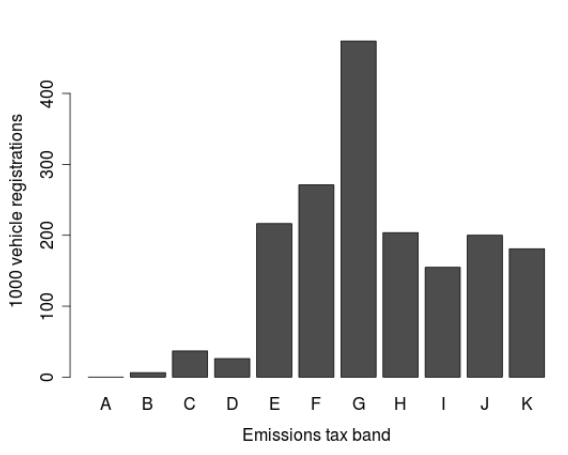
\includegraphics[width = 9 cm]{ebandsperc}}
 \caption[Barpolt of 2001 car registrations by emission band]
 {Barpolt of 2001 car registrations by emission band
(England and Wales). Raw data from DfT).} \label{febandsperc}
\end{figure}

From this analysis, the energy use of vehicles in England and
Wales in 2001 calculated as 2.40 MJ/vkm. This is almost 20\% lower than the figure
calculated for the 2011 fleet (which should be \emph{more} energy efficient)
in \cref{sdirecte} and the figure of used by \citet{MacKay2009}.
The value is slightly closer to the fleet efficiency estimates based on
\citet{Decc2011t} for 2001 (2.89 MJ/vkm).
% Footnote here??? no
As alluded to by the Vehicle
Certification Agency (2011), such differences are not unexpected: real world use
(reported in \citet{Decc2011t})
is different from controlled tests. Another explanation for the low energy use
value is that the average efficiency of new cars has been improving over time
so a lower value for cars registered since 2001 is to be expected, compared
with cars registered before 2001, for which no emissions data is available:
the data presented in \cref{febandsperc} represents new cars sold in 2002, and do not
include any of the car fleet that was on the road during 2001. The use of this
data as a proxy for 2001 fleet efficiencies may be justified, however, by the
relatively high correlation between estimated fleet efficiencies of wards, from
year to year (\cref{ffleetscat}, \cref{tfleetscat}).

\begin{figure}
\centering{ 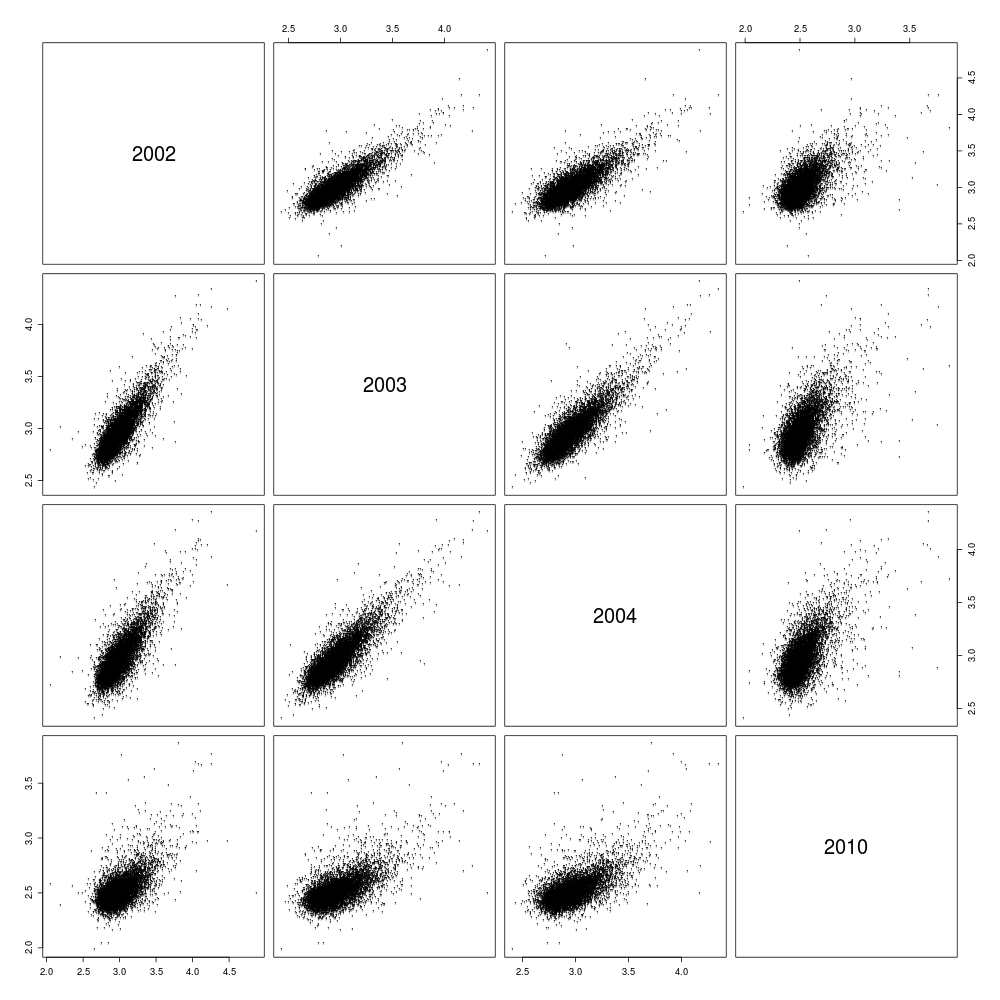
\includegraphics[width = 14 cm]{fleetscat}}
 \caption[Scatterplots of estimated fleet efficiencies at MSOA level]
 {Scatterplots of estimated fleet efficiencies at MSOA level in England
and Wales (MJ/km, both axes). Note the declines in correlation over time.
See appendix DFT data for details on the construction of this graph.)
} \label{ffleetscat}
\end{figure}

\begin{table}[htbp]
\caption[Correlation matrix of estimated fleet efficiencies, 2002-2010]
{Pearson's correlation matrix of fit between estimated efficiencies,
2002-2010, based on DfT data at the MSOA level in England and Wales. Some years
omitted for simplicity.}
\begin{center}
\begin{tabular}{rrrrrrr}
\toprule
& \textbf{2002} & \textbf{2003} & \textbf{2004} &
\textbf{2006} & \textbf{2008} & \textbf{2010} \\
\midrule
\textbf{2002} & 1.00 & 0.85 & 0.81 & 0.77 & 0.70 & 0.61 \\
\textbf{2003} & 0.85 & 1.00 & 0.86 & 0.81 & 0.72 & 0.64 \\
\textbf{2004} & 0.81 & 0.86 & 1.00 & 0.84 & 0.74 & 0.64 \\
\textbf{2006} & 0.77 & 0.81 & 0.84 & 1.00 & 0.77 & 0.67 \\
\textbf{2008} & 0.70 & 0.72 & 0.74 & 0.77 & 1.00 & 0.71 \\
\textbf{2010} & 0.61 & 0.64 & 0.64 & 0.67 & 0.71 & 1.00 \\ \bottomrule
\end{tabular}  \end{center}
\label{tfleetscat}
\end{table}

In light of these considerations, the regional emissions band data seem to be
better placed as a way of providing weights for adjusting the
national average fleet efficiency, rather than absolute estimates of
fleet efficiency. Caution should be used when interpreting the results,
acknowledging the fact that the 2002 data is much more sparse on
emissions estimates because the majority of cars in the vehicle fleet
were registered before emission bands were introduced.
% energy analysis will be done with and without efficiency considerations.
The raw
data on which MSOA level fleet efficiency estimates are based was provided by
the DfT in 5 variables (\cref{tefraw}).\footnote{Thanks to Daryl Lloyd,
who created the bespoke dataset
used for this purpose.
% (See Appendix \ref{ap:fleetcalc}).
}

\begin{table}[htbp]
\caption[The first 5 rows of the raw DfT emissions band data]
{The first 5 rows of the raw DfT emissions band data. All 1.3 million
rows are available online at \href{http://ubuntuone.com/6inKDTsdhLkFQNat0O6QOK}
{http://ubuntuone.com/6inKDTsdhLkFQNat0O6QOK}}
\begin{center}
\begin{tabular}{llrlr}
\toprule
MidSOA & BodyType & \multicolumn{1}{l}{Year} & CO2Group & \multicolumn{1}{l}{N} \\
\midrule
E02004277 & CARS & 2005 & Band C: 111 - 120 & 21 \\
E02001092 & CARS & 2007 & Band I: 176 - 185 & 6 \\
E02005251 & OTHERS & 2011 & non-cars & 4 \\
E02005506 & CARS & 2004 &  & 3 \\
E02003897 & CARS & 2007 & Band F: 141 - 150 & 26 \\
\bottomrule
\end{tabular} \end{center}
\label{tefraw}
\end{table}

Once this data had been re-arranged into a more manageable form, converted into
an efficiency estimate using \cref{ebands}, and re-weighted to reflect the nation-wide
average fleet efficiency of 3 MJ/vkm,
% (Appendix DftData – the same as the one with
% time correlations),
a subset including only 2002 registrations from MSOAs within
Yorkshire and the Humber was taken. These calculations suggest the region's car fleet is more
efficient than the national average, although only by 3\% (2.9 vs 3.0 MJ/km, respectively).
Plotted at the regional scale, these estimates coincide with the expected trend for rich
and rural areas to have relatively inefficient car fleets (\cref{fig:espace}).
% (hence the ``gas guzzlers'' stereotype).
% (ref, + which is more important, wealth of rurality? => correlation) (Fig. x).

\begin{figure}[htbp]
  \centerline{
    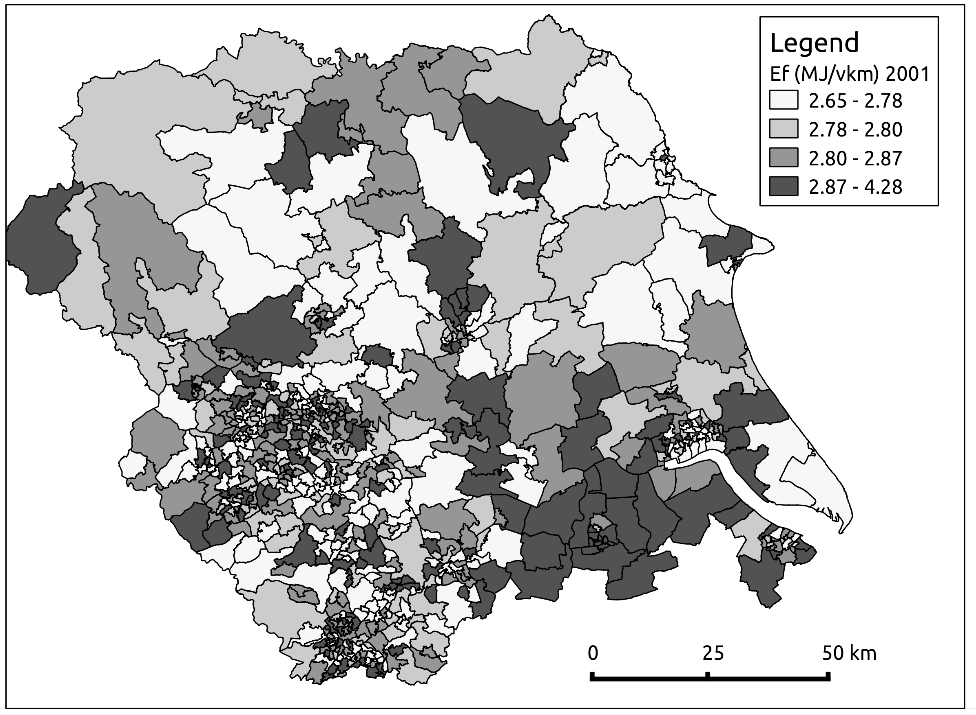
\includegraphics[width = 14 cm]{espace.png}}
  \caption[Car fleet efficiencies in Yorkshire and the Humber in 2001]{Car fleet
efficiencies in Yorkshire and the Humber in 2001. Data from DfT.
% Method of calculation described in  \cref{ap:fleetcalc}
}
  \label{fig:espace}
\end{figure}

Vehicle efficiency is clearly an important determinant of the energy costs of
personal transport, and \cref{fig:espace} demonstrates that it does vary over space in a
(more or less) predictable way. However, it is important to keep the relative
ranges of these variations in context. The deviation from the mean of the most
and least efficient car fleets at the MSOA level is only 25\% and 27\% respectively. This
variability is far less than the difference between the efficiencies of
different transport modes (see \cref{ffinale} below,
where 30 and 10-fold differences exists between the
fuel requirements of cars and bicycles for direct and system level fuel use
respectively) and less than variability in the distances that people travel
to work. Due to the risk of `double counting' the impact of fleet efficiency
(through the size of car variable and these fleet efficiency estimates),
the fact that these fleet efficiencies are not distance weighted and
the relatively minor variability of fleet efficiencies overall,
this spatial dimension was not initially included in the energy cost
calculations presented in the subsequent section.
A method for including local fleet efficiencies has been demonstrated
and this could be of use for policy makers developing locally targeted
transport interventions, researchers aiming to create more
spatially aware scenarios of the future and even businesses and 
3$^{rd}$ sector organisations marketing and advocating low-energy
transport solutions. %!!! footnote for each!!!
% (where an xx\% difference exists between the areas that commute least, and most
% far, compared with the average )(ref).\footnote{Thanks to Daryl Lloyd,
% who created the bespoke dataset
% used for this purpose.
% (See Appendix \ref{ap:fleetcalc}).
% }

% % Removed as it's not necessary, but is time consuming re-add elsewhere???
% \section{Real vs reported efficiencies} \label{sreale}
% The above efficiency calculations depend on the assumption that the EU tests
% from which official energy efficiency data is derived apply to the real world.
% However, this idea has been criticised by a number of sources.%!!! sources
% Most recently, a large (n > 30,000, and growing) self-selected survey of actual
% fuel consumption on British roads has been undertaken by the motoring website
% honestjohn.co.uk. The findings suggest that cars' fuel economy (measured in
% miles per gallon) may, on average, be only 88\% of their official stated values
% \citep{Brignall2013-careff}.

\section{Final energy use estimates} \label{sfinal} \index{energy use}
This final section concludes the chapter on energy costs of personal travel
with our final ``best estimates'' of energy costs. Four types of energy
costs are included: direct energy use of the vehicle ($Ef$, calculated
in \cref{sdirecte}), and three indirect components of system level energy
use ($Esys$): the energy used in fuel production ($Efp$) and the embedded
energy of vehicles and guideways ($Ev$ and $Eg$, see \cref{ssystemlevel}).
The results are presented in \cref{tfinale}. Due to the importance of these
estimates for the results of our model, these results are also presented
visually, in \cref{ffinale}. It is interesting to compare these estimates
with estimates of fuel use of different modes made independently of this
study, over 20 years ago (\cref{fmjpkm1991}).

\begin{table}[htbp]
\caption[Final estimates of the direct and indirect energy use of 8 modes]{Final
estimates of the direct and indirect energy use of the eight
most common modes of travel to work (10, including three car types),
presented in MJ/pkm, under average occupancy rates for Great Britain
(except for cars, which have units of MJ/vkm).}
\begin{center}
\begin{tabular}{lrrrrr}
\toprule
Mode & \multicolumn{1}{l}{Ef} & \multicolumn{1}{l}{Efp} & \multicolumn{1}{l}{Ev} & \multicolumn{1}{l}{Eg} & \multicolumn{1}{l}{Esys} \\
\midrule
Bicycle & 0.09 & 0.541 & 0.05 & \multicolumn{1}{l}{-} & 0.7 \\
Bus (local) & 2.1 & 0.85 & 0.15 & 0.30 & 3.4 \\
Car (small) & 2.5 & 0.99 & 0.57 & 0.30 & 4.3 \\
Car (average) & 3.0 & 1.21 & 0.67 & 0.30 & 5.2 \\
Car (large) & 3.9 & 1.58 & 0.87 & 0.30 & 6.7 \\
Coach & 0.43 & 0.17 & 0.08 & 0.30 & 1.0 \\
Motorbike & 1.7 & 0.70 & 0.33 & 0.30 & 3.1 \\
Train  & 0.77 & 0.31 & \multicolumn{1}{l}{-} & \multicolumn{1}{l}{-} & 1.1 \\
Tram & 0.57 & 0.38 & \multicolumn{1}{l}{-} & \multicolumn{1}{l}{-} & 1.0 \\
Walking & 0.13 & 0.75 & \multicolumn{1}{l}{-} & \multicolumn{1}{l}{-} & 0.9 \\ 
\bottomrule
\end{tabular}\end{center}
\label{tfinale}
\end{table}

\begin{figure}[h]
 \centering
 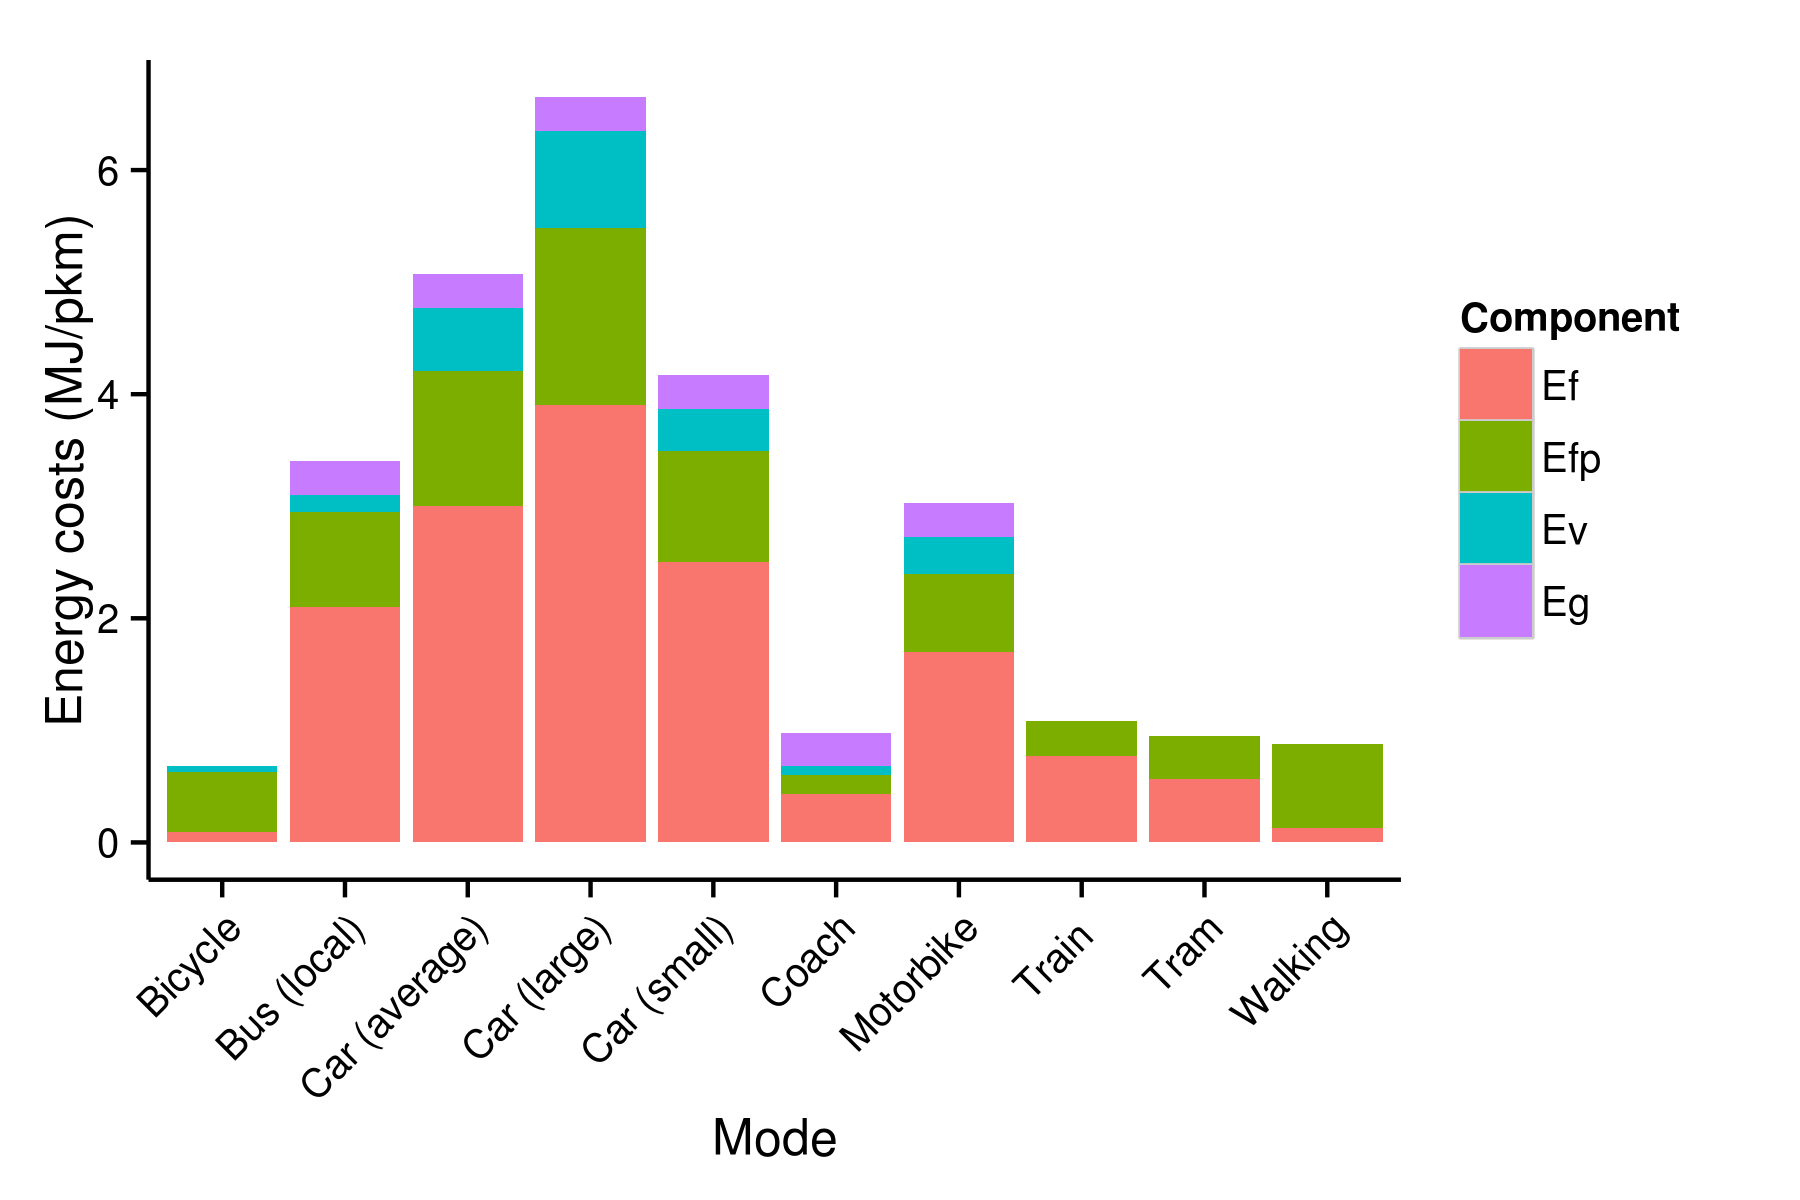
\includegraphics[width=14cm]{finale}
 % cc-trans.png: 1113x529 pixel, 72dpi, 39.26x18.66 cm, bb=0 0 1113 529
 \caption{Final energy use estimates, from a range of sources.}
 \label{ffinale}
\end{figure}

\begin{figure}[h]
 \centering
 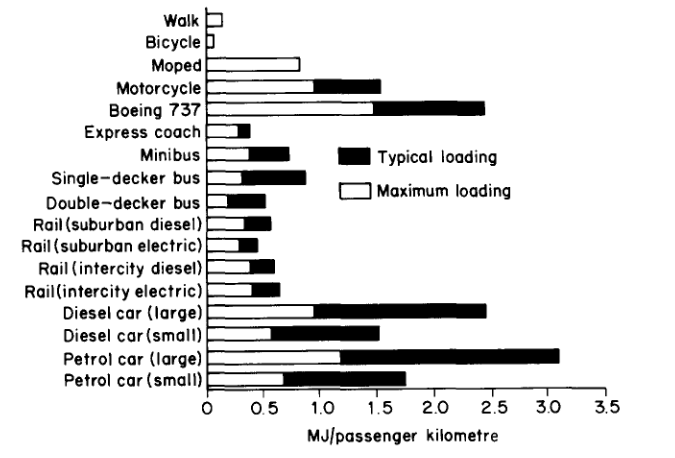
\includegraphics[width=14cm]{mjpkm1991}
 \caption[Fuel energy use of UK transport modes, 1991]
 {Estimated fuel energy use of UK transport modes, from \citet{Hughes1991149}.}
 \label{fmjpkm1991}
\end{figure}

These values provide the $EI$ values by mode that are fed into the model
to calculate energy costs by trip. Although the larger system level energy costs
are deemed more realistic, the majority of the analysis presented in \cref{Chapter6}
to \cref{Chapter8} include only direct energy costs. This decision was made
because the direct energy costs are more certain, come from official data sources and
currently coincide with the UK's reporting of transport emissions
Direct energy use should thus be more relevant to transport planners needing to meet energy and climate
targets in the short-term.\footnote{In
the UK and the European Union as a whole, this legislation
comes primarily from the EU's 20/20/20 targets: 20\% reduction
in emissions, 20\% of final energy delivered from renewable sources and
a 20\% increase in energy efficiency.
}
Longer-term scenarios 
are less constrained by such reporting conventions, so the scenarios
presented in \cref{Chapter8} use system level energy use estimates.
Overall, the impact estimating energy use at the system level
including system level on relative energy use is minor, as it scales
proportionally with direct energy use for all modes of transport.


% Short section of tables summarising the energy use input data
% Build on .odf file of this section.
% Abrupt end !!!